% Currently this document is written in German
% !TeX spellcheck = de_DE

%Ensure that all odl school LaTeX habits are remarked
\RequirePackage[l2tabu, orthodox]{nag}
%Neue deutsche Trennmuster
%Siehe http://www.ctan.org/pkg/dehyph-exptl und http://projekte.dante.de/Trennmuster/WebHome
%Nur für pdflatex, nicht für lualatex
\RequirePackage[ngerman=ngerman-x-latest]{hyphsubst}
\documentclass{lni}
% in Englisch stattdessen:
%\documentclass[english]{lni}







%% Some packages, no need to be adabted

% enable copy and paste of ligatures (e.g., in "workflow" and umlauts)
\usepackage{cmap}

%Überschrift des Literaturverzeichnisses
%Only in German
\iflnienglish
\else
\renewcommand{\refname}{References}
\fi

%Enable input of umlauts using UTF-8.
\usepackage[utf8]{inputenc}

\usepackage{graphicx}
\usepackage{fancyhdr}
\usepackage{tikz}
\usepackage{tikz-qtree}
\usepackage{mathtools}

\newlength\dualpgfwidth
\setlength\dualpgfwidth{.5\linewidth}

\usepackage{pgfplots}

%!TEX root=paper.tex
\usepackage{tikz}

\usepackage{amssymb}
\usepackage{amsmath}

\usepackage{newfloat}
\DeclareFloatingEnvironment[
  fileext=lol,
  name=Listing
]{listing}

\usepackage[labelformat=simple]{subcaption}

\DeclareCaptionSubType{listing}
\renewcommand\thesublisting{(\alph{sublisting})}

\newcommand{\code}[1]{\texttt{#1}}

\newlength\dualpgfwidth
\setlength\dualpgfwidth{.5\linewidth}

\usepackage{pgfplots}
\pgfplotsset{compat=1.14}

%Kopf- und Fußzeileneinstellungen
\fancypagestyle{lnifirstpage}{
% Löscht alle Kopf- und Fußzeileneinstellungen
\fancyhf{}

%Kopfzeile
\fancyhead[RO]{\small Submission to BTW'17}
%Für den Herausgeber:
%\fancyhead[RO]{\small <Vorname Nachname [et. al.]> (Hrsg.): <Buchtitel>,\linebreak%
%Lecture Notes in Informatics (LNI), Gesellschaft für Informatik, Bonn <Jahr> \hspace{5pt} \thepage \hspace{0.05cm}}

%Linie unter Kopfzeile
\renewcommand{\headrulewidth}{0.4pt}
}

% Put in the short title (Kurztitle) here
\fancypagestyle{lni}{
\fancyhf{}
%Zu lange Titel müssen von den HerausgeberInnen gekürzt werden, Vorschläge der AutorInnen dazu sind herzlich willkommen.
\fancyhead[RO]{\small Gilbert: Declarative Sparse Linear Algebra on Massively Parallel Dataflow Systems\hspace{5pt}
\thepage \hspace{0.05cm}}
\fancyhead[LE]{\hspace{0.05cm}\small \thepage \hspace{5pt}
%Bis zu drei AutorInnen werden alle angeführt, darüber hinaus wird nur die erste Autorin bzw. der erste Autor angeführt und alle Weiteren mit et al.\ abgekürzt.
%Zu lange AutorInnenlisten müssen von den HerausgeberInnen gekürzt werden.
Till Rohrmann, Sebastian Schelter, Tilmann Rabl and Volker Markl}
\renewcommand{\headrulewidth}{0.4pt}
}

%if lstlistings is used
%better approach: use the minted package - see https://en.wikibooks.org/wiki/LaTeX/Source_Code_Listings#The_minted_package
\usepackage{listings}

%\iflnienglish
%\usepackage[figurename=Fig., tablename=Tab.]{caption}
%\else
%\usepackage[figurename=Abb., tablename=Tab., small]{caption}
%\fi

% Listingname heißt nun List.
\renewcommand{\lstlistingname}{List.}

%for easy quotations: \enquote{text}
\usepackage{csquotes}

\usepackage[T1]{fontenc}

%enable margin kerning
\usepackage{microtype}

%for demonstration purposes only
\usepackage[math]{blindtext}

%tweak \url{...}
\usepackage{url}
%nicer // - solution by http://tex.stackexchange.com/a/98470/9075
\makeatletter
\def\Url@twoslashes{\mathchar`\/\@ifnextchar/{\kern-.2em}{}}
\g@addto@macro\UrlSpecials{\do\/{\Url@twoslashes}}
\makeatother
\urlstyle{same}
%improve wrapping of URLs - hint by http://tex.stackexchange.com/a/10419/9075
\makeatletter
\g@addto@macro{\UrlBreaks}{\UrlOrds}
\makeatother

%diagonal lines in a table - http://tex.stackexchange.com/questions/17745/diagonal-lines-in-table-cell
%slashbox is not available in texlive (due to licensing) and also gives bad results. Thus, we use diagbox
%\usepackage{diagbox}

\usepackage{booktabs}

%required for pdfcomment later
\usepackage{xcolor}

% new packages BEFORE hyperref
% See also http://tex.stackexchange.com/questions/1863/which-packages-should-be-loaded-after-hyperref-instead-of-before

%enable hyperref without colors and without bookmarks
\usepackage[
%pdfauthor={},
%pdfsubject={},
%pdftitle={},
%pdfkeywords={},
bookmarks=false,
breaklinks=true,
colorlinks=true,
linkcolor=black,
citecolor=black,
urlcolor=black,
pdfpagelayout=SinglePage,
pdfstartview=Fit
]{hyperref}
%enables correct jumping to figures when referencing
\usepackage[all]{hypcap}

%enable nice comments
\usepackage{pdfcomment}
\newcommand{\commentontext}[2]{\colorbox{yellow!60}{#1}\pdfcomment[color={0.234 0.867 0.211},hoffset=-6pt,voffset=10pt,opacity=0.5]{#2}}
\newcommand{\commentatside}[1]{\pdfcomment[color={0.045 0.278 0.643},icon=Note]{#1}}

%compatibality with TODO package
\newcommand{\todo}[1]{\commentatside{#1}}

%enable \cref{...} and \Cref{...} instead of \ref: Type of reference included in the link
\iflnienglish
\usepackage[capitalise,nameinlink]{cleveref}
%Nice formats for \cref
\crefname{section}{Sect.}{Sect.}
\Crefname{section}{Section}{Sections}
\crefname{figure}{Fig.}{Fig.}
\Crefname{figure}{Figure}{Figures}
\else
\usepackage[ngerman,capitalise,nameinlink]{cleveref}
\fi

%introduce \powerset - hint by http://matheplanet.com/matheplanet/nuke/html/viewtopic.php?topic=136492&post_id=997377
\DeclareFontFamily{U}{MnSymbolC}{}
\DeclareSymbolFont{MnSyC}{U}{MnSymbolC}{m}{n}
\DeclareFontShape{U}{MnSymbolC}{m}{n}{
    <-6>  MnSymbolC5
   <6-7>  MnSymbolC6
   <7-8>  MnSymbolC7
   <8-9>  MnSymbolC8
   <9-10> MnSymbolC9
  <10-12> MnSymbolC10
  <12->   MnSymbolC12%
}{}
\DeclareMathSymbol{\powerset}{\mathord}{MnSyC}{180}

%improve float placement
%source: http://people.cs.uu.nl/piet/floats/node1.html
%see also: http://tex.stackexchange.com/a/35130/9075
\renewcommand{\textfraction}{0.05}
\renewcommand{\topfraction}{0.95}
\renewcommand{\bottomfraction}{0.95}
\renewcommand{\floatpagefraction}{0.35}
\setcounter{totalnumber}{5}

% correct bad hyphenation here
\hyphenation{net-works semi-conduc-tor}


%%% Adapt to your needs from here

%Beginn der Seitenzählung für diesen Beitrag
\setcounter{page}{1}

\author{
Till Rohrmann\footnote{Affiliation, name@email.com} \, %
Sebastian Schelter\footnote{Technische Universität Berlin, sebastian.schelter@tu-berlin.de} \, %
Tilmann Rabl\footnote{Technische Universität Berlin / DFKI, rabl@tu-berlin.de} \, %
Volker Markl\footnote{Technische Universität Berlin / DFKI, volker.markl@tu-berlin.de} \, %
}

\title{Gilbert: Declarative Sparse Linear Algebra\\ on Massively Parallel Dataflow Systems}

\begin{document}
\maketitle

%hint by http://tex.stackexchange.com/a/30229/9075 and http://tex.stackexchange.com/a/247652/9075
\thispagestyle{lnifirstpage}
\pagestyle{lni}

%Auf Anzahl der AutorInnen setzen, damit die weitere Nummerierung der Fußnoten passt
%Dieser Befehl \verb|\setcounter{footnote}{2}| legt in dem Fall fest, dass 2 Fußnotennummern bereits für die AutorInnen verbraucht wurden, damit die darauf folgenden Fußnoten mit der richtigen Nummerierung (ab 3) fortfahren. Dieser Wert muss an die jeweilige Zahl an AutorInnen bzw. bereits verbrauchte Fußnoten angepasst werden, sofern im weiteren Verlauf Fußnoten verwendet werden.
\setcounter{footnote}{2}

\begin{abstract}
In recent years, the generated and gathered data has increased at an almost exponential rate. At the same time, people realized its usefulness in terms of insights it can provide. However, lifting the true treasures requires powerful analysis tools, since the insights are buried deep below a pile of meaningless data. Unfortunately, our analytic capacities did not scale well with the growing data. Most of our existing tools run only on a single computer and thus are limited by its memory. The most promising remedy to deal with large-scale data is to exploit parallelism.

We propose Gilbert, a distributed sparse linear algebra system, to solve the imminent lack of analytic capacities. Gilbert offers a MATLAB-like programming language for linear algebra programs, which are automatically executed in parallel. Transparent parallelization is achieved by compiling the linear algebra operations first into an intermediate representation. This language-independent representation is amenable to high-level algebraic optimizations.
Different optimization strategies are evaluated and the best one is chosen by a cost-based optimizer. The optimized intermediate representation is then transformed into a suitable format for parallel execution. Gilbert generates execution plans for Spark and Stratosphere, two massively parallel dataflow systems, and can easily be extended to support further parallel execution engines. Distributed matrices are represented by square blocks to guarantee a well-balanced trade-off between data parallelism and data granularity.

Exhaustive evaluation indicates that Gilbert is able to process varying amounts of data exceeding the memory of a single computer on clusters of different sizes.
Three famous machine learning (ML) algorithms, namely PageRank, k-Means and Gaussian non-negative matrix factorization (GNMF), were implemented with Gilbert.
That emphasizes Gilbert's support for distributed iterations, an essential prerequisite for a broad set of ML algorithms. The performance of these algorithms is compared to optimized implementations based on Spark and Stratosphere. Even though Gilbert is not as fast as the optimized algorithms, it simplifies the development process significantly due to its high-level programming language.
\end{abstract}

\begin{keywords}
Dataflow Optimization, Linear Algebra, Distributed Dataflow Systems
\end{keywords}

%!TEX root=paper.tex
\section{Introduction}

%In order to develop Big Data solutions, one has to solve multifaceted problems. %The necessary technology stack comprises the recording of data, the data cleaning, the meta-data generation, the representation and integration with other data sources, the analysis and modeling of the actual problem as well as the interpretation. Each task for itself is highly complex and deserves an individual paper.
%For us, the data analysis part is the key aspect in solving Big Data problems. Henceforth, we will concentrate on how to gain valuable insights from a huge data set. Once big data sets were amassed, people quickly recognized that these sets contain valuable information they only have to harness. 
Key component of modern big data solutions are a sophisticated analysis algorithms.% In this work, we focus on the data analysis part of the problems. 
Unfortunately, the search for useful patterns and peculiarities in large data sets resembled the search for a needle in a haystack. This challenge requires tools that are able to analyze vast amounts of data quickly. Most of these tools are based on statistics to extract interesting features. It is beneficial to apply these statistical means to the complete data set instead of smaller chunks. Even if the chunks cover the complete data set, important correlations between data points might get lost if chunks are treated individually. Moreover, the statistical tools improve their descriptive and predictive results by getting fed more data. The more data is available, the more likely it is that noise cancels out and that the significant patterns manifest. However, these benefits come at the price of an increased computing time, which requires fast computer systems to make computations feasible. 
%The insights gained from collected data already help to govern business decisions, improve life quality or simply create new industries from scratch.
%For example, retail stores analyze their sales, customer, pricing and weather data in order to decide which products to offer or when to do a discount sale. That not only increases the revenue of the shops but also boosts the satisfaction of the customers by getting better offers. 
%Police departments try to detect probable crime sites by extracting patterns from previously recorded criminal acts and then reinforce the policemen in that region~\cite{lohr:yt2012a}.
%The intelligent deployment of policemen improves security for citizens without having to hire more officers.
%Hospitals analyze their patients' records and scientific studies in order to find the cancer treatment best complying with the specifics of the patient. The individual therapy maximizes the chance of cure~\cite{watson:2013a}.
%Another example showing the benefits of data analysis made it even into a Hollywood film.
%The film Moneyball is based on the true story of the Oakland Athletics baseball team, whose management built an elite team in an unfavorable financial situation. They employed sophisticated data analysis methods to spot underestimated players, who they could cheaply recruit.
%That marked the start of sports statistics, which are nowadays a common tool for professional teams.
%These examples emphasize the importance and utility of information gained with analytic tools from gathered data.
%Interestingly, the IDC, an international market research firm, estimates that only $0.5\%$ of the globally collected data is harnessed~\cite{gantz:iaf2012a}. They further state that about $23\%$ of today's data is worth being analyzed. Thus, there is still potential left for improvements.

%What are the reasons for the huge gap between actual and dormant exploitation?
%One of the reasons is that we are lacking the tools to keep up the pace of how fast data is created and collected.
Analysis tools traditionally do not scale well for vast data sets.
%The more data a system has to process, the longer it will take to finish.
Because of the exponential data growth, analytic capacities have to improve at a similar speed to keep analyses feasible. 
%In order to decrease the runtime of our analytic tools there are two adjusting screws. First of all, there are the algorithms.
By finding an algorithm with a lower runtime complexity than an existing algorithm, e.g., for clustering, run times can be drastically decreased. 
However, it is often not possible to develop better algorithms for certain problems. In some cases, it is even proven that there exists a lower bound for any algorithm solving the problem.
%Thus, certain problems have an inherent limitation of how fast they can be computed. 
The other way to speed up the analytic tools is to make the computer faster by vertical or horizontal scaling. To scale vertically means that we add more resources to a single computer.
For example, the main memory size or the CPU frequency of a computer can be increased to increase computational power.
In contrast to that, horizontal scaling means to add more computer nodes to a system.
By having more than one node, the work can be split up and distributed across the nodes.
If each split is smaller than the original problem, the system can process it faster. %In recent years, we have seen that clock rates of CPUs stagnated.
%Before, there was a simple receipt to increase the computing power of micro-controllers; increase the clock rate, which demands more power, and shrink the channel widths to mitigate for the increased power consumption.
%However, the shrinkage induces the problem of leakage, which increases the power demand again.
%The consumed power is limited by the amount of energy that can be dissipated and thus there is a technological limit for the increase of clock rate.
%When it became clear that the micro-controller would hit this so-called ``power wall'', one duplicated the micro-controller's functionality to support simultaneous execution of multiple applications and to harness the inherent parallelism of programs.
The emerging multi-core and distributed systems pose new challenges for programmers.%, since now they have to know about locking, deadlocks, race-conditions and inter-process communication in order to make most of the available hardware.
Since they have to be able to reason about interwoven parallel control flows, parallel program development is highly cumbersome and error-prone.
Therefore, new programming models are conceived, a development that relieves the programmer from the tedious low-level tasks related to parallelization such as load-balancing, scheduling of parallel tasks, and fault recovery.
With this new models, programmers can concentrate on the actual algorithm and use case rather than reasoning about distributed systems. These are the reasons why Google's MapReduce~\cite{dean:c2008a} framework and its open source re-implementation Hadoop~\cite{hadoop:2008a} became so popular among scientists as well as engineers.
%MapReduce is a programming framework for concurrent computations on vast amounts of data running on a large cluster.
%Its ingenious idea was to separate the computation into a \emph{map} and a \emph{reduce} phase.
%In the map phase, the input data set is split into elements which are all processed independently.
%Afterwards, the results of the mapper are grouped together and each produced group is given to a reducer.
%The reducer knows about all elements in his group and produces the final result.
%The strengths of MapReduce are that it is expressive enough to implement a multitude of different algorithms while facilitating at the same time parallel execution.
However, MapReduce and other frameworks force the user to express the program in a certain way, which is often not natural or intuitive to a user coming from a different domain.
Especially, in the field of data analytics and machine learning programs are usually expressed in a mathematical form.
Therefore, systems such as MATLAB~\cite{matlab} and R~\cite{r:1993a} are widely used and recognized for their fast prototyping capabilities and their extensive mathematical libraries.
However, these linear algebra systems lack proper support for automatic parallelization on large clusters and are thus restricting the user to a single workstation.
Therefore, the amount of processable data is limited to the size of the main memory, which constitutes a serious drawback for real-world applications.

\begin{figure}[t!]
\centering
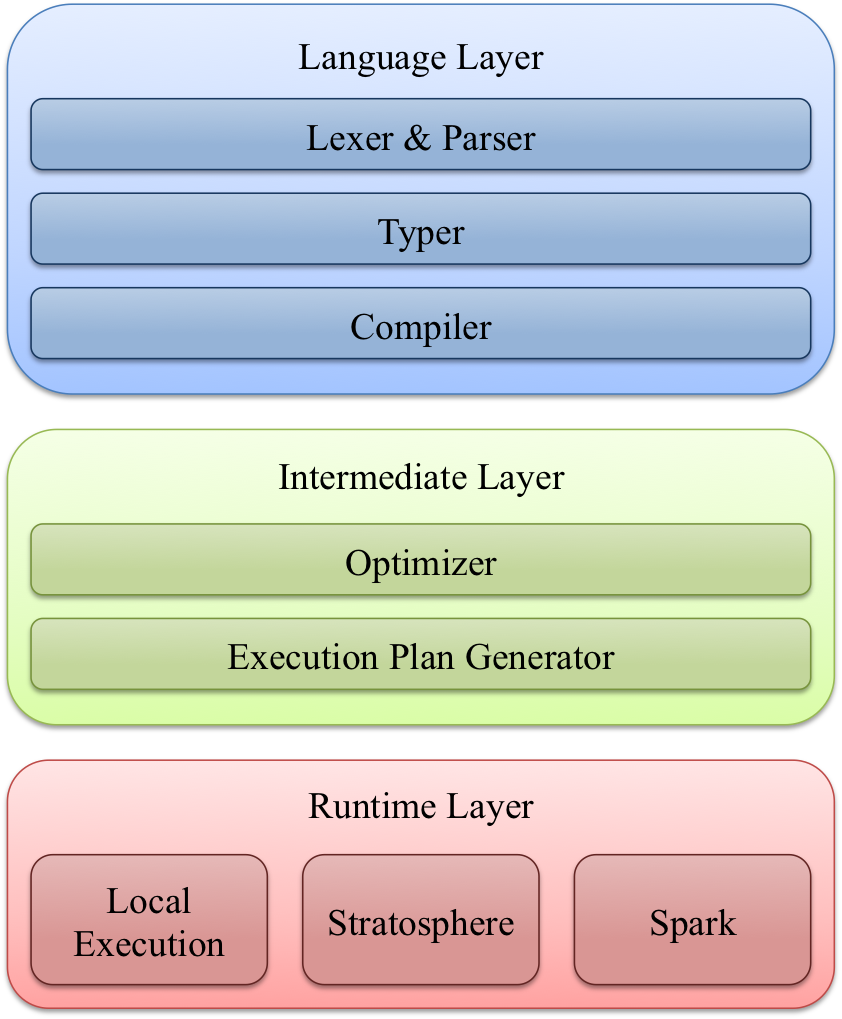
\includegraphics[height=0.175\paperheight]{images/systemArchitecture.png}
\caption{The layered system architecture of Gilbert. The language layer is responsible for parsing, typing and compiling the given Matlab code. The intermediate layer facilitates high-level optimization strategies. The runtime layer is responsible for executing the specified program in parallel.}
\label{fig:systemArchitecture}
\end{figure}

As a solution we propose Gilbert, a distributed sparse linear algebra environment. Gilbert provides a Matlab-like language for distributed sparse linear algebra operations. It has a layered architecture, which is shown in Figure \ref{fig:systemArchitecture}. The first layer is the language layer. It contains all functionality to parse the given Gilbert code and to compile it into an intermediate representation (IR). The second layer is the intermediate layer and it receives the IR of the Gilbert code. The intermediate format is the ideal representation to apply language independent high-level transformations. The Gilbert optimizer applies several algebraic optimizations prior to the generation of the execution plan. The execution plan generator translates the optimized IR into a specific execution plan, depending on the selected execution engine. Once the program has been translated into an execution engine's specific plan, it is executed on the respective back end. 

Our main contributions are:
\begin{itemize}
 \item Gilbert allows to write MATLAB-like code for sparse linear algebra and execute it on massively parallel dataflow systems.
 \item Its expressiveness allows to quickly develop scalable algorithms to analyze web-scale data.
 \item We introduce a novel fixed-point operator which replaces loops by recursion and can be efficiently parallelized.
 \item Furthermore, we demonstrate that dataflow optimizers can be used to automatically select an good matrix multiplication strategy. 
\end{itemize}
%Gilbert provides a Matlab-like language for distributed sparse linear algebra operations. %Being such a system, it comprises the complete stack of functionalities necessary to implement a programming language. At first, the system has to divide the given source code into tokens. These tokens are parsed and an abstract syntax tree (AST) is created. In order to generate the intermediate representation (IR), type information is needed for all expressions. This information is extracted by the typing system. Knowing the types, the compiler can translate the Gilbert program into its IR. The IR is well suited to apply high-level transformations to the program. At last, the execution plan generator translates the IR into an execution plan which can be executed in parallel. %The layered system architecture is shown in \cref{fig:systemArchitecture}. 

%%It has a layered architecture. The first layer is the language layer. It contains all functionality to parse the given Gilbert code and to compile it into an intermediate representation (IR). The second layer is the intermediate layer and it receives the IR of the Gilbert code. The intermediate format is the ideal representation to apply language independent high-level transformations. The Gilbert optimizer applies several algebraic optimizations prior to the generation of the execution plan. The execution plan generator translates the optimized IR into a specific execution plan, depending on the selected execution engine. Once the program has been translated into an execution engine's specific plan, it is executed on the respective back end.

%\begin{figure}[t!]
% \centering
% 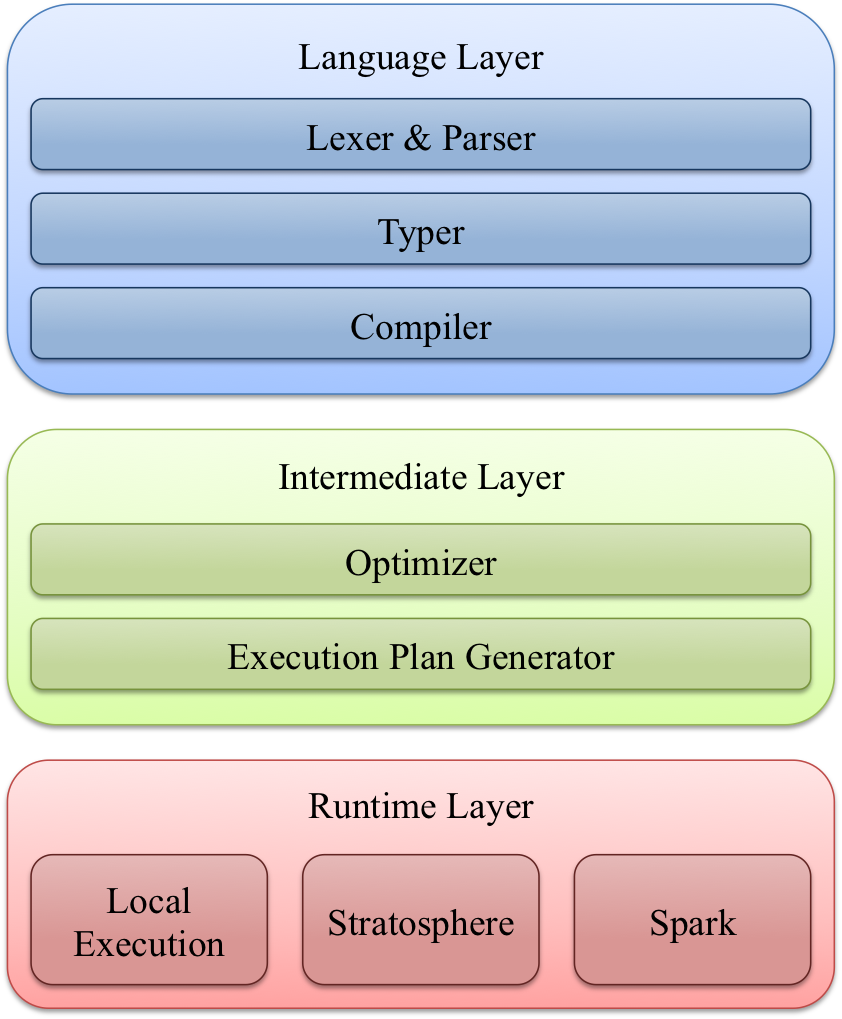
\includegraphics[height=0.175\paperheight]{images/systemArchitecture.png}
% \caption{The layered system architecture of Gilbert. The language layer is responsible for parsing, typing and compiling the given Matlab code. The intermediate layer facilitates high-level optimization strategies. The runtime layer is responsible for executing the specified program in parallel.}
% \label{fig:systemArchitecture}
%\end{figure}

%%\textbf{Language Layer}. The language layer contains all the logic for translating Gilbert source code into the intermediate representation, see the subsequent section for more details. %Gilbert's supported language and its features is described in \cref{sec:gilbertLanguage}.
%%The resulting AST is attributed with type information by the typing system. The typer makes use of the Hindley-Milner algorithm to automatically infer types.%, as it is described in~\cref{sec:hmInference}. 
%%The type information enriched AST is then translated into a front end independent representation of linear algebra operations, namely the IR. The format Gilbert uses to represent linear algebra operations in a generalized format is described in Section~\ref{sec:intermediaterepresentation}.

%%\textbf{Intermediate Layer}. The intermediate layer contains the optimizer and the execution plan generator. The optimizer applies the optimizations described in Section~\ref{sec:gilbertOptimizer} to IR of the Gilbert program. Then the IR is translated into the execution engine's specific format. The linear algebra operations are translated into a dataflow graph as explained in Section~\ref{sec:LinearAlgebraOperations}. The system supports Flink and Spark as parallel execution engines.

The rest of this paper is structured as follows. %In \ref{sec:overview} we give an overview of Gilbert.
%Then, 
In \Cref{sec:gilbertFeatures}, Gilbert's language and its features are described.
\Cref{sec:gilbertRuntime} presents how linear algebra operations are mapped to a dataflow system. Gilbert's performance and scalability is evaluated in \Cref{sec:evaluation}.
Related work is covered in \Cref{sec:relatedWork} before the work is concluded in \Cref{sec:conclusion}.
\section{Gilbert Language}
\label{cha:gilbertlanguage}

Prior to the actual start of development of Gilbert, we had to decide which higher-level language Gilbert should support.
Since Gilbert aims to be a sparse linear algebra environment, R and MATLAB are the natural candidates.
In fact, R and MATLAB are quite similar and are both widely used in academics as well as industry to develop mathematical programs.
Due to their expressiveness and their rich library support with myriads of mathematical functions, they are just as well suited for quick prototyping as it is for full-fledged development.
In combination with their ease of use, they quickly became the standard in industry for numerical processing.
Our final choice fell on MATLAB, because of our higher familiarity with this language.
Yet, we believe that there are no fundamental reasons which would prohibit the support of R.
In fact, the translation from one language to the other should be straight-forward on the compiler level.

Another reason to imitate an existing language and not to devise a new language geared towards parallel execution is the laziness of people.
Since its part of human nature to be sluggish, people are initially unwilling to learn new things or to re-adapt.
Therefore, Gilbert was conceived to require as little re-adaption as possible of users familiar with MATLAB.
We believe that this aspect is a crucial property of Gilbert in order to be successfully adopted by the statistical community.
Furthermore, a neat side effect is that existing MATLAB code can almost seamlessly be ported to Gilbert and thus benefits instantaneously from the computational power of a large shared nothing cluster.
This feature becomes particularly relevant considering the huge existing code base.
Re-coding parts of it would be prohibitive, because of the required labor and provoked costs.

In the following sections, we will describe the key aspects of the Gilbert language and explain the design decisions taken.
Subsequently, we will give a formal specification of the Gilbert language and describe the used parser.

\subsection{Language Features}
\label{sec:languageFeatures}

In order to not be overwhelmed by the complexity of MATLAB but still support a full functional subset of it, Gilbert was restricted to support the following language features and data types.
We decided to keep the feature set as small as possible to concentrate on the parallelization instead of supporting hardly used language features.
The elementary data type of linear algebra and therefore also of MATLAB is a matrix.
Gilbert supports arbitrary $2$-dimensional matrices whose elements can be \emph{double} or \emph{boolean}.
Vectors are not represented by a special type but instead are treated as a matrix.
Additionally, scalar \emph{double} and \emph{boolean} values are supported.
The reason to introduce a \emph{boolean} type is the control flow of loops, being covered in a later paragraph.
Since Gilbert has to interact with data stored on disk, strings are supported.

Gilbert also implements cell array types.
A cell array consists of indexed data containers, called cells.
Each cell can contain an individual data type.
Therefore, cell arrays can be used to pass multiple data items combined as one argument to a function or to obtain multiple items from a function.
The latter aspect is particularly important, because Gilbert only supports functions with a single return value.
A cell array is defined using curly braces and commas to separate individual values.
The cells can be accessed by an index appended in curly braces to the cell array variable.
\Cref{lst:cellArray} shows how to define and access them.
The formal definition of the syntax of cell arrays can be found in \cref{sec:languageGrammar}.
In contrast to MATLAB's cell arrays, though, Gilbert only allows to have $1$-dimensional arrays.
However, this constraint does not impose a serious restriction, since all multi-dimensional arrays can be transformed into $1$-dimensional arrays. 

\begin{listing}[!h]
  \begin{CenteredBox}
    \begin{lstlisting}[language=Matlab,
        commentstyle=\color{black},
        stringstyle=\color{black},
    ]
c = {true, 2*2, 'cell', 'array'};
b = c{1} & false; % = false
d = c{2} ^ 2; % = 16
s = {c{4}, c{3}}; % = {'array', 'cell'} 
    \end{lstlisting}
  \end{CenteredBox}
  \caption{Cell array usage in Gilbert. Definition of a 4 element cell array which is accessed subsequently.}
  \label{lst:cellArray}
\end{listing}

Gilbert supports the basic linear algebra operations defined on matrices and scalars.
They include among others the common operations \code{+}, \code{-}, \code{/} and \code{*}, whereas \code{*} denotes the matrix-matrix multiplication and all other operations are interpreted cellwisely.
The cellwise multiplication is indicated by a point preceding the operator as it is common for cellwise operations in MATLAB.
Gilbert also supports comparisons operators such as \code{>}, \code{>=}, \code{==} and \code{\textasciitilde=}.
These operators become handy for realizing dynamic termination criteria for loops.
The full set of supported mathematical operations can be found in appendix 1.

Besides the basic arithmetic operations, the user can also define named functions and anonymous functions.
This feature not only enables a better structure of the code but also allows to express second-order functions.
The syntax of anonymous functions adheres to the MATLAB syntax.
An anonymous function which calculates the sum of its input squares could be defined as follows: \code{@(x,y) x*x + y*y}.
A formal definition can be found in \cref{sec:languageGrammar}.

An important aspect of MATLAB are loops.
MATLAB permits the user to express \code{for} and \code{while} loops.
However, these loops are quite powerful in the sense that they allow iterations with side effects.
The problem of parallelization of iterations with side effects is that the referenced external state has to be maintained.
This circumstance makes preprocessing and execution unnecessarily complex.
For the sake of simplicity, Gilbert is limited to a different loop mechanism.
Gilbert offers a fixpoint operator \code{fixpoint}, which iteratively applies a given update function $f$ on the previous result of $f$, starting with an initial value $x$ at iteration $0$.
Thus, the $n^{th}$ iteration is equivalent to applying the function $f$ $n$ times to $x$: 
\begin{displaymath}
  n^{th}\text{ iteration}\equiv\underbrace{f(f(\ldots(f(x))\ldots))}_{\text{$n$ times}}
\end{displaymath}

In order to terminate the fixpoint operation, the operator provides two mechanisms.
First of all, the user has to specify a maximum number \code{m} of iterations after which the loop is terminated.
This mechanism is henceforth denoted as the \emph{static termination criterion}.
Such a termination criterion is often not sufficient for machine learning algorithms, because they usually continue their computations until they have reached a certain convergence criterion.
Since the number of iterations necessary to reach this state is not always known a priori, it is called the \emph{dynamic termination criterion}.
Gilbert offers support for the dynamic termination criterion.
The user can provide a convergence function \code{c} to the fixpoint operator.
The convergence function is called with the previous and current fixpoint value and returns a boolean value, indicating whether the termination criterion has been fulfilled or not.
Thus, the fixpoint operator terminates either if convergence was detected or if the maximum number of iterations is exceeded.
Consequently, the fixpoint operator is defined as follows:
\begin{equation}
fixpoint: \underbrace{T}_{\text{\code{x}}} \times \left( \underbrace{T \rightarrow T}_{\text{\code{f}}} \right) \times \underbrace{\mathbb{N}}_{\text{\code{m}}} \times \left(\underbrace{T\times T \rightarrow \mathbb{B}}_{\text{\code{c}}} \right) \rightarrow T
\label{eqn:fixpoint}
\end{equation}
with $T$ being a generic type variable.

In fact, the fixpoint operator replaces iterations by recursions whereas the update function $f$ is pure.
At this point Gilbert breaks with existing MATLAB code.
To make Gilbert a real subset of MATLAB, the fixpoint operator would have to be integrated into MATLAB.
The integration could easily be done by providing an external library with the definition of the fixpoint function.

Even though the iteration operator restricts the set of valid programs in Gilbert, it is still expressive enough to support a wide variety of programs.
Moreover, all MATLAB programs can be transformed so that the for and while loops are replaced by the fixpoint operator.
This replacement is simply achieved by passing all data that is read or written to as parameters to the update function.
The update function returns the same set of variables, just with updated values.
Such an exemplified transformation can be seen in \cref{fig:for2Fixpoint}.
Here we can see that all data that is operated on is passed to the fixpoint operator as a cell array.
Lines $1-2$ of \cref{fig:for2Fixpoint:fixpoint} define the update function \code{f}.
The parameter \code{x} is a cell array whose first entry contains the accumulator \code{A} and second entry is the loop counter \code{i}.
In line $2$ we see the returned cell array value of the anonymous function.
The first entry is the sum of the current accumulator value and the loop counter.
The second entry is the incremented loop counter for the next iteration.
Line $3$ calls the fixpoint operator with the initial cell array value, the update function and the maximum number of iterations.
The final result is retrieved from the final cell array value in line $4$.

\begin{listing}
  \centering
  \begin{sublisting}{.4\linewidth}
    \begin{lstlisting}[language=Matlab,
      commentstyle=\color{black},
      stringstyle=\color{black},
      keywordstyle=\color{black}\bfseries,
    ]
A = 0;
for i = 1:10
  A = A + i;
end
    \end{lstlisting}
    \caption{For loop}
    \label[listing]{fig:for2Fixpoint:for}
  \end{sublisting}
  \begin{sublisting}{.5\linewidth}
      \begin{lstlisting}[language=Matlab]
f = @(x) ...
  {x{1} + x{2}, x{2} + 1};
r = fixpoint({0,1}, f, 10);
A = r{1};
    \end{lstlisting}
    \caption{Fixpoint}
    \label[listing]{fig:for2Fixpoint:fixpoint}
  \end{sublisting}
  \caption{Transformation from Matlab for loop \subref{fig:for2Fixpoint:for} to Gilbert fixpoint \subref{fig:for2Fixpoint:fixpoint} formulation. Essentially, all iteration data is combined and passed as a cell array value to the update function.}
  \label{fig:for2Fixpoint}
\end{listing}

\subsection{Language Grammar}
\label{sec:languageGrammar}

We could not find an official specification of the MATLAB language.
Therefore, we defined our own grammar with the goal to imitate MATLAB as closely as possible.
Even though we extensively tested the conformity of the language, we cannot guarantee that it is completely equivalent.
In the following, we give the Backus-Naur form (BNF) of the Gilbert language.

%\setlength{\grammarindent}{12em} % increase separation between LHS/RHS
\begin{lstlisting}
<program> ::= <stmtOrFuncList>

<stmtOrFuncList> ::= (<stmt> | <funcDef>)*

<stmt> ::= <assignment> | <expression>

<assignment> ::= <lhs> '=' <rhs>

<lhs> ::= <identifier>

<rhs> ::= <expression>

<funcDef> ::= 'function' <funcValues>? <identifier> <funcParams> <funcBody> 'end'

<funcValues> ::= <identifier> '='
\alt '[' <identifier> (',' <identifier>)* ']' '='

<funcParams> ::= '(' ')'
\alt '(' <identifier> (',' <identifier>)* ')'

<funcBody> ::= <stmtOrFuncList>

<expression> ::= <aexp1>

<aexp1> ::= <aexp2> ('||' <aexp2>)*

<aexp2> ::= <aexp3> ('\&\&' <aexp3>)*

<aexp3> ::= <aexp4> ('|' <aexp4>)*

<aexp4> ::= <aexp5> ('\&' <aexp5>)*

<aexp5> ::= <aexp6> (<compOp> <aexp6>)*

<aexp6> ::= <aexp7> (':' <aexp7>)*

<aexp7> ::= <aexp8> (<addOp> <aexp8>)*

<aexp8> ::= <aexp9> (<multOp> <aexp9>)*

<aexp9> ::= <prefixOp> <aexp9> | <aexp10>

<aexp10> ::= <aexp11> (<expOp> <aexp11>)*

<aexp11> ::= <unaryExpression> <postfixOp>?

<unaryExpression> ::= <elemExpression> | '(' <expression> ')'

<elemExpression> ::= <funcApplication> \alt <cellExpression> \alt <identifier> \alt <scalar> \alt <booleanLiteral> \alt <matrix> \alt <stringLiteral> \alt <anonymousFunc> \alt <funcReference>

<funcApplication> ::= <identifier> '(' ')'
\alt <identifier> '(' <expression> (',' <expression>)* ')'

<funcReference> ::= '@' <identifier>

<cellExpression> ::= <cellArray> | <cellArrayIndexing>

<cellArray> ::= '\{' <expression> (',' <expression>)* '\}'

<cellArrayIndexing> ::= <identifier> ('\{' <numericLiteral> '\}')+

<scalar> ::= <numericLiteral>

<matrix> ::= '[' <matrixRow> (<newlineOrSemicolon> <matrixRow>)* ']'

<matrixRow> ::= <expression> (',' <expression>)*

<prefixOp> ::= '+' | '-'

<multOp> ::= '*' | '/' | '.*' | './'

<addOp> ::= '+' | '-'

<compOp> ::= "'<'" | "'<='" | "'>'" | "'>='" | "'=='" | "'~='"

<postfixOp> ::= '.'' | '''

<expOp> ::= '.\textasciicircum'

<newlineOrSemicolon> ::= NL | ';'

\end{lstlisting}

For the sake of simplicity, we have left out most of the whitespace and line break handling.
Furthermore, we used notations known from regular expressions to shorten the grammar specification.
We use parentheses to group subexpressions and apply the following multiplicity specifiers: \code{*}, \code{+} and \code{?}.
The semantics of these specifiers can be found in \cref{tab:multiplicity}.

\begin{table}[!h]
  \centering
  \begin{tabular}{c|l}
  Multiplicity specifier & Meaning\\
  \hline
  $\langle exp \rangle$* & $\langle exp\rangle$ can appear multiple times \\
  $\langle exp\rangle$+ & $\langle exp\rangle$ can appear multiple times but at least once \\
  $\langle exp\rangle$? & $\langle exp\rangle$ can appear exactly once or not at all
  \end{tabular}
  \caption{Multiplicity specifier used to specify the Gilbert language. They are borrowed from regular expressions.}
  \label{tab:multiplicity}
\end{table}

The different \emph{aexp} non-terminals are used to model the precedence order of the mathematical operators.
An overview of the precedence can be found in \cref{tab:precedences}.
The $'$ operator denotes the transpose of the operand.

\begin{table}[!h]
  \centering
  \begin{tabular}{l|l}
  Operator class & Operators\\
  \hline
  Short circuit logical or & $||$\\
  Short circuit logical and & $\&\&$\\
  Logical or & $|$ \\
  Logical and & $\&$ \\
  Comparators & $>$, $>=$, $<$, $<=$, $==$, \textasciitilde$=$\\
  Range operator & $:$ \\
  Addition and Subtraction & $+$, $-$\\
  Multiplication and Division & $*$, $/$\\
  Prefix operator & $+$, $-$\\
  Exponentiation & \textasciicircum\\
  Postfix operator & $'$
  \end{tabular}
  \caption{Precedence order of mathematical operators in ascending order.}
  \label{tab:precedences}
\end{table}

The non-terminals \emph{identifier}, \emph{numericLiteral}, \emph{stringLiteral} and \emph{booleanLiteral} are tokens generated by the lexer. The corresponding tokens are defined by regular expressions and can be found in \cref{tab:tokens}.

\begin{table}[!h]
  \centering
  \begin{tabular}{l|l}
  Token name & Regular expression\\
  \hline
  identifier & [a-zA-Z] [a-zA-Z0-9\_]*\\
  numericLiteral & [+-]? [0-9]+ (.[0-9]*)? ([eE][+-]?[0-9]+)? | [+-]? .[0-9]+ ([eE][+-]?[0-9]+)? \\
  stringLiteral & "[\textasciicircum"]*" | '[\textasciicircum']*'\\
  booleanLiteral & true | false
  \end{tabular}
  \caption{Definition of generated tokens by regular expressions.}
  \label{tab:tokens}
\end{table}

\subsection{Parser}

In order to implement Gilbert, a parser had to be selected which is powerful enough to parse the Gilbert language.
Luckily, the language is rather simple and since none of the production rules is left recursive, we can use a simple LL(n) parser.
This aspect becomes important when we justify our implementation choices in \cref{cha:implementation}.

The attentive reader will have noticed that our language specification contains an ambiguity.
Consider, for example, the following valid MATLAB code \code{A' + B'} where \code{A} and \code{B} are matrices.
The code should produce the sum of two transposed matrices.
However, on the lexer level the two transpose operators will be recognized as the enclosing apostrophes of a string literal.
Therefore, the lexer will produce an identifier token followed by a string literal token.
Eventually, these tokens will cause a parser error, because there is no production rule consuming such a combination of tokens.

In order to solve this problem, we have to differentiate a transpose operator from an apostrophe belonging to a string literal.
Since the transpose operator always follows after an expression, we can check that the previously detected token is an identifier, closing parentheses, closing bracket or closing brace.
If one of these cases is true, then the apostrophe is considered to be a transpose operator.
Otherwise, it belongs to a string literal.
%!TEX root=main.tex
\subsection{Gilbert Typing}
\label{cha:gilberttyping}

Program development in general is an error-prone and time-consuming task.
Besides the actual development phase, it usually involves several iterations of bug fixing.
In order to reduce the number of pitfalls a programmer can fall into, typing systems were developed.
Typing systems assign a \emph{type} to language constructs such as variables, functions and expressions.
That way, the system gives meaning to an otherwise vacuous program.
In the memory of a computer, everything is represented as a sequence of bits, no matter whether it is an instruction code, memory address, character, boolean or floating-point number.
For a computer there is no way to intrinsically differentiate between the different meanings without an additional hint.
This hint comes in the form of types.
Knowing that a bit sequence represents a floating-point number, the computer is aware of the valid values and operations and can check for its correct usage.

The pursued goal in typing theory is to develop a system which detects erroneous program behavior and is at the same time \emph{sound} and \emph{complete}.
Soundness means that if a program passes the typer, then it behaves correctly.
Completeness means that if a program behaves correctly, then it will pass the typer.
However, it turned out that typing systems need to be extremely sophisticated in order to detect non-trivial errors and as a result they are often undecidable for non toy example languages.
For example, consider the division operation.
The code \code{1/0} would be well-typed by almost all common type checkers, because integers are divisible.
However, the code will cause a runtime error because of division by zero.
In order to detect this type of error, the type checking would have to be far more detailed.
Therefore, the constraints are usually relaxed.
In general, current type systems can already detect many different errors but they are still incomplete and only partially sound.

Type checking can be distinguished into two categories: \emph{static} and \emph{dynamic} type checking.
Static type checkers work on the source code and assign a type to each expression at compile-time.
If it detects any typing incompatibilities, such as providing the wrong arguments to a function call, assigning conflicting data types or to apply not supported operations, the type checker will alert the programmer.
Most type checkers are designed to act conservatively, meaning that they relax the constraints of soundness and completeness for the sake of decidability.
It is easy to see that the typing problem can be reduced to the halting problem, if soundness and completeness are assumed.
For this purpose consider \cref{lst:typingHaltingProblem}.
In order to decide whether this code is well- or ill-typed, the typer has to decide whether \code{f} halts.
Since the halting problem is undecidable, also the set of programs producing a runtime type error is undecidable.
\begin{listing}[!h]
	\begin{CenteredBox}
		\begin{lstlisting}[language=C++,
		commentstyle=\color{black},
		stringstyle=\color{black},
		keywordstyle=\color{black}\bfseries,
		]
if(willHalt(f)){
	code_with_type_error;
}else{
	code_without_type_error;
}
		\end{lstlisting}
	\end{CenteredBox}
	\caption{In order to type this code fragment, the typer has to solve the halting problem.}
	\label{lst:typingHaltingProblem}
\end{listing}

In contrast to static typing, dynamic type checkers enrich each object with some kind of type tag which is used to check type compatibility at runtime.
However, possible errors are only recognized after the corresponding code has been executed.
A more thorough discussion about the advantages and disadvantages of both paradigms follows in \cref{sec:staticVSDynamic}.
In practice, there is hardly any static typing system which does not rely at least partially on dynamic typing as well.
Dynamic downcasts, for instance, as they are common in \code{C++}, can only be implemented by checking whether the underlying type is the target type or a subtype of it.

\subsection{Static Typing vs. Dynamic Typing}
\label{sec:staticVSDynamic}

Static type checking analyzes the program prior to execution to detect errors.
This approach has the advantage that possible programming mistakes are caught early in the development process.
An assignment of a string to a double would be an example for such a mistake.
As indicated by \cite{westland:jss2002a}, who investigated the influence of errors during the software development process, unfixed errors become exponentially more costly with each phase.
Therefore, it is important to detect and correct errors as soon as possible.
Static typing usually requires the user to specify types explicitly in the source code, because the language lacks type inference or has ambiguities which prevent the type inference from inferring the correct types.
Java, for example, does not have type inference and therefore the user has to specify types redundantly.
In line $1$ of \cref{lst:javaTypeAnnotation}, it is obvious that we have to specify twice the type \code{Object}, even though this type can easily be deduced from the right side of the assignment.
Furthermore, in line $4$ we see an addition of two integers.
It is clear that the result is an integer and thus the \code{int} type specifier is dispensable.
\begin{listing}[!h]
	\begin{CenteredBox}
		\begin{lstlisting}[language=C++,
		  commentstyle=\color{black},
		  stringstyle=\color{black},
		  keywordstyle=\color{black}\bfseries,
		  ]
Object obj = new Object();
int a = 1;
int b = 0;
int c = a + b;			
		\end{lstlisting}
	\end{CenteredBox}
	\caption{Type annotations in Java.}
	\label{lst:javaTypeAnnotation}
\end{listing}

Proponents of static typing emphasize that explicit type information, as they occur in Java and many other programming languages, documents the code.
It is easier for a programmer to use existing code if he can identify function arguments and their types with one glance, for instance. 
Additionally, it is possible for the compiler to apply sophisticated optimization techniques, if it knows the types.
By operating on these values, the compiler could, for example, use more efficient machine instructions for floating-point calculations.
Furthermore, it is possible to substitute virtual function calls for direct calls, if the actual object type is known.
Another benefit of static typing is the increased type safety.
After passing the type checker, the program is guaranteed to fulfill for all inputs some set of type safety properties.
This guarantee frees the runtime from checking the safety properties and thus the program can be executed more efficiently.
Type information additionally helps to provide a better programming experience in an IDE by offering type dependent context help.
If the IDE knows the type of a variable, then it can tell the programmer which methods are supported by this type, for instance.
And last but not least, explicit typing permits a better abstraction of functionality and, thus, increases modularity.
Interfaces can be defined to orchestrate the interaction between several software components allowing them to be developed independently from each other.

In contrast to these arguments, advocates of dynamic typing argue that their approach is more vivid and better suited for prototyping, because the static typing approach is too rigid.
These aspects come especially into effect for programs in a highly dynamic environment with unknown or quickly changing requirements such as data integration.
Another advantage is that the compile time is reduced because of fewer passes the compiler has to go through.
However, the avoided type checks will then be realized within the runtime which adds overhead.
But the dynamic nature allows interpreters to dynamically load code more quickly, because all type checkings are deferred until its actual execution.
Moreover, dynamic languages support duck typing as a powerful tool to write reusable code.
The term duck typing originates from the poet James Whitcomb Riley, who stated: \enquote{When I see a bird that walks like a duck and swims like a duck and quacks like a duck, I call that bird a duck.}~\cite{heim:2007a}.
Essentially, duck typing means that not the actual type of an object decides whether a program is well- or ill-typed but the set of supported methods and its properties.
For example, consider a function which calls a method \code{count} on its given parameter.
Then all function calls are valid which are called with an argument having a method \code{count}, independently of its actual type.
That way, the programmer can write code which is applicable for a wide variety of types without having to specify them explicitly.
\cite{ousterhout:c1998a} even claims that static typed languages do not guarantee a higher type safety than dynamic typed languages.
Furthermore, he states that they are more verbose and it is difficult to write reusable code.
However, it is unclear in which way reducing language features leads to a more powerful and expressive language. 

The debate of whether statically or dynamically typed languages are superior has almost reached religious character.
It is likely that none of the approaches alone solves all the problems.
Instead, a combination of the strengths of both paradigms promises the best results~\cite{meijer:2004a}.

We are in the unfortunate situation that MATLAB belongs to the class of dynamically typed languages and Gilbert requires type information for its parallel execution.
The parallel data processing systems, used to run Gilbert programs, have to know which data types are passed from one worker node to another.
Therefore, the MATLAB language has to be enriched with type information.

It exists research of how to add explicit type information to MATLAB.
For example, \cite{hendren:2011a} introduced the special keyword \emph{atype} to MATLAB which is understood and interpreted by an extended compiler.
The \emph{atype} keyword basically acts as a type annotation and can be implemented within a special library or as a weaver.
Even though this approach seems quite promising, we decided to opt for a more transparent mechanism, namely type inference.
Type inference has the advantage that the MATLAB user is not bothered by having to add explicit type information and thus can continue writing his code in the usual fashion.
In case that the type inference algorithm cannot properly infer the types, there has to be a way to resolve this problem.
We decided to pursue a similar approach as \cite{furr:2009a}.
\cite{furr:2009a} added type information to Ruby by adding special comments to the respective code sections.
Thereby, the code does not break with the Ruby standard and still contains type information.
As typing system, we use the Hindley-Milner (HM) type system~\cite{hindley:tams1969a,milner:jcss1978a} and a slightly derived form of algorithm W~\cite{damas:1982a} for type inference.
Algorithm W will be described in the next section in detail.
Even though there exist more powerful type systems than the HM type system, it has the appealing charm that the algorithm W is sound, complete and decidable with respect to the type system.
Furthermore, it has proven to type several algorithms implemented within Gilbert correctly.

\subsection{Hindley-Milner Type Inference}
\label{sec:hmInference}

The Hindley-Milner (HM) type inference assigns types to expressions.
It was initially developed to type functional languages.
In fact, HM type inference was first implemented as the typing part of the programming language ML.
HM types the expressions of the lambda calculus enriched with the \code{let}-expression.
For a detailed review of the lambda calculus, the interested reader is referred to the article of \cite{cardone:hhl2006a}.

The set of expressions $e$ contains variables, function applications, function abstractions and \code{let}-expressions.
The formal definition of $e$ is
\begin{eqnarray*}
e &= & x\quad\text{(Variable)}\\
&|& e\ e\quad\text{(Application)}\\
&|& \lambda x. e\quad\text{(Abstraction)}\\
&|& \code{let } x = e \code{ in } e
\end{eqnarray*}
For those unconversant with lambda expressions, we will quickly revise them.
The function application is written as $e_1\ e_2$ whereas $e_1$ denotes a function and $e_2$ the function argument which is applied to the function body.
The function abstraction $\lambda x.e$ is the equivalent of an anonymous function, as it is known from many program languages.
It is initiated with a $\lambda$ followed by its function parameter $x$ and the function body $e$.
The let-expression $\code{let } x = e_1 \code{ in } e_2$ introduces a new variable $x$, having the value $e_1$, into the context $\Gamma$.
This variable can be used within the expression $e_2$.
The semantic of the assignment is that every occurrence of $x$ in $e_2$ is replaced by $e_1$.
The context $\Gamma$ contains all type information so far known and is a mapping from variables to types.
A more precise definition is given in a later paragraph.

One might think that the lambda calculus is only a toy language and that the set of expressions is not expressive enough to represent any common programming problem.
However, it turned out that the lambda calculus is Turing complete and thus any programming language can be reduced to it.
Therefore, it is enough to reason about the typing aspects of these expressions.

Even though Gilbert is not a functional language, we can use the HM type inference to compute the types at compile-time.
The only difference to the above defined set of expressions is that Gilbert does not have a \code{let}-expression.
Instead, it has ordinary assignments of the form $x = e$.
The notion of the assignment is similar to the \code{let}-expression.
An assignment adds a new variable $x$ with the value $e$ to the context.

HM type inference distinguishes between two sorts of types, \emph{mono}- and \emph{polytypes}.
Monotypes $\tau$ are defined as follows:
\begin{eqnarray*}
\tau &=& \alpha\quad\text{(Variable)}\\
&|& D\ \tau\ \ldots \tau\quad\text{(Application)}
\end{eqnarray*}

A monotype always denotes a concrete type.
If the type is known, it can be a type constant, such as \code{int}, \code{float} or \code{string}, or a parametric type.
A parametric type takes itself type arguments to form a concrete type.
An example of a parametric type is the \code{Set} or the \code{List} which can be instantiated with arbitrary element types.
Type constants are a special case of the application rule with an empty list of arguments.
If the type is not yet known but can only be a single type, then a type variable $\alpha$ is used.
Often, it can be the case that these type variables are replaced with known types at a later stage of the type inference.

In contrast to monotypes, polytypes $\sigma$ denote multiple types.
They are defined by
\begin{eqnarray*}
\sigma &=& \tau \\
&|& \forall \alpha .\sigma
\end{eqnarray*}

A type of the form $\forall \alpha.\sigma$ denotes the set of all types where $\alpha$ is substituted by a concrete type $\tau$ within $\sigma$.
Consider, for example, the tuple access function \code{fst} which takes a tuple and returns the first entry.
The function \code{fst} should be applicable to all different types of tuples, for example $(\code{int}, \code{int})$, $(\code{string}, \code{float})$, etc.
If \code{fst} has a monotype, then it will only work for one concrete tuple type.
Therefore, \code{fst} has a polytype.
The actual type of \code{fst} is $\forall \alpha,\beta . (\alpha, \beta) \rightarrow \alpha$.
Depending on the applied tuple argument the quantified type variables are instantiated respectively.
Polytypes permit to implement generic functions in a type safe manner and that is called parametric polymorphism.
It is important to note that polytypes introduce ambiguities with respect to the calculated type.
An expression having the type $\forall \alpha. \alpha$ also has the type $\code{int}$, for example.
Thus, the latter type would be a valid inferred type, even though the first one is more general.
In order to dissolve this ambiguities, the typing system always looks for the most general type.

Usually, expressions depend on other expressions and thus their types.
Therefore, a type dictionary is maintained where types of expressions are stored, which already have been seen while parsing the code.
And that is exactly what the context $\Gamma$ is used for.
$\Gamma$ contains a list of pairs $x:\sigma$, which are called assumptions.
The formal definition of $\Gamma$ is
\begin{eqnarray*}
\Gamma &=& \Gamma, x:\sigma \\
&|& \epsilon\ \text{(empty)}
\end{eqnarray*}

Having defined the context, expressions and types, the typing judgment $\Gamma \vdash x : \sigma$ can be explained.
The typing judgment can be interpreted that given the context $\Gamma$ the variable $x$ has the type $\sigma$.
The way how to come up with these judgments is defined by deduction rules.
Before taking a closer look at them, some auxiliary functions are first introduced.

An important distinction in an HM type expression is the state of the type variables.
In general, type variables can appear as \emph{free} or as \emph{bound} variables.
A type variable $\alpha$ is called bound if it occurs in an expression of the form $\forall \alpha. \tau$.
$\forall$ binds the subsequent variable in the context of the expression.
All variables which are not bound are free.
We can define a function $free$ which calculates the set of free type variables in a type expression and in the type context.
\begin{eqnarray*}
free(\alpha) &=& \{\alpha\}\\
free(D\ \alpha_1\ \ldots\ \alpha_n) &=& \bigcup_{i=1}^n free(\alpha_i)\\
free(\forall \alpha. \tau) &=& free(\tau) \setminus \{\alpha\}\\
free(\Gamma) &=& \bigcup_{x:\sigma \in \Gamma} free(\sigma)
\end{eqnarray*}

\subsection{Algorithm W}

The algorithm W was initially developed by \cite{damas:1982a} and allows to solve the HM type inference in almost linear time with respect to the size of the source code....
% Thus, it is also applicable to large programs.
% A modified version of the original algorithm which incorporates side effects into the deduction rules is presented.
% Even though these side effects contradict the purity of logical deduction rules, it allows to express the algorithm concisely.
% The algorithm W is defined by the following deduction rules:

% \begin{prooftree}
% 	\AxiomC{$x : \sigma \in \Gamma$}
% 	\AxiomC{$\tau = inst(\sigma)$}
% 	\LeftLabel{Variable:\quad}
% 	\BinaryInfC{$\Gamma \vdash x : \tau$}
% \end{prooftree}

% \begin{prooftree}
% 	\AxiomC{$\Gamma \vdash e_0 : \tau_0$}
% 	\AxiomC{$\Gamma \vdash e_1 : \tau_1$}
% 	\AxiomC{$\tau^\prime=newvar$}
% 	\AxiomC{$unify(\tau_0, \tau_1 \rightarrow \tau^\prime)$}
% 	\LeftLabel{Application:\quad}
% 	\QuaternaryInfC{$\Gamma \vdash e_0 e_1 : \tau^\prime$}
% \end{prooftree}

% \begin{prooftree}
% 	\AxiomC{$\tau = newvar$}
% 	\AxiomC{$\Gamma,x:\tau \vdash e : \tau^\prime$}
% 	\LeftLabel{Abstraction:\quad}
% 	\BinaryInfC{$\Gamma \vdash \lambda x.e:\tau \rightarrow \tau^\prime$}
% \end{prooftree}

% \begin{prooftree}
% 	\AxiomC{$\Gamma \vdash e_0 : \tau$}
% 	\AxiomC{$\Gamma, x : \overline{\Gamma}(\tau) \vdash e_1 : \tau^\prime$}
% 	\LeftLabel{Assignment:\quad}
% 	\BinaryInfC{$\Gamma \vdash x = e_0; e_1 : \tau^\prime$}
% \end{prooftree}

% Each rule has the form
% \begin{tabular}{c}
% Premise\\
% \hline
% Conclusion
% \end{tabular}, which means that if the premise can be proven, then the conclusion is true.

% Let us go step by step through the different deduction rules of the algorithm.
% The first rule says that a variable $x$ has the type $\tau$, if an assumption of $x$ in $\Gamma$ whose type $\sigma$ can be specialized to $\tau$ is found.
% The function $inst$ does the specialization of the type.
% A type is specialized by removing all quantifiers and replacing the bound variables by fresh monotype variables.

% The second rule deals with function applications.
% In order to show that a function application has the type $\tau^\prime$, we first have to look at the function type $\tau_0$ and the argument type $\tau_1$.
% In order to fulfill the conclusion, we know that the type of $e_0$ has to be a function with an argument of type $\tau_1$ and some result type $\tau^\prime$.
% If the type $\tau_0$ is equivalent to this function type $\tau_1\rightarrow\tau^\prime$, we can deduce that the resulting type is $\tau^\prime$.
% The equivalence is tested by the $unify$ function.
% This function takes two types and tries to find the most general type unifying both arguments.

% The $unify$ function is an essential part of the typing system, since it incorporates all constraints imposed by the different expressions in order to find the most general type validating the program.
% The working principle can be best understood by looking at its pseudocode in \cref{lst:unify}.
% \begin{listing}[!h]
% 	\begin{CenteredBox}
% 		\begin{lstlisting}[language=ML,
% 		commentstyle=\color{black},
% 		  stringstyle=\color{black},
% 		  keywordstyle=\color{black}\bfseries,
% 		  morekeywords={def, return},
% 		  deletekeywords={type, of, with, and}
% 		]
% def unify(typeA: Type, typeB: Type): Type = {
% 	val tA = resolve(typeA)
% 	val tB = resolve(typeB)

% 	if( at least one term is a type variable){
% 		return union(tA, tB)
% 	}
%     else if( both type expressions are of the form D p1 ... pn with 
% 		the same D and the number of arguments){
% 		return D(unify(tA.p1, tB.p1), ..., unify(tA.pn, tb.pn))
% 	} else{
% 		return typeMismatch
% 	}
% }
% 		\end{lstlisting}
% 	\end{CenteredBox}
% 	\caption{$Unify$ function.}
% 	\label{lst:unify}
% \end{listing}

% First of all, both type expressions are resolved.
% This means that type variables, which are contained as sub expressions, are looked up in the type variable assignment dictionary.
% This dictionary maintains the current assignments between variables and their types.
% If a type variable has an assigned type, then this type is substituted for the corresponding type variable.
% If at least one of the resulting type expressions is still a type variable, then we can simply construct the union of both types.
% The union function returns the more concrete type of both arguments and updates the dictionary correspondingly.
% Thus, if both arguments are type variables, then one of them is returned.
% If only one argument is a type variable, then the other argument is returned.

% If none of the resolved type expressions is a type variable, then they have to be a type application.
% Applications can only be unified if they are constructed by the same function symbol and if they have the same number of arguments.
% If this condition is fulfilled, the arguments can be unified.
% Depending on the unifiability of the arguments, the overall type application is unifiable or not.

% If both type expressions are constructed by different type applications, then the types are impossible to unify.
% Consequently, a type mismatch error will be returned.

% The third rule allows to type lambda abstractions or in Gilbert's case concrete and anonymous functions.
% In order to show that a lambda abstraction $\lambda x.e$ has the type $\tau\rightarrow \tau^\prime$, a new type variable for the unknown parameter type is introduced.
% After adding this assumption to the context, the type of the function body $e$ has to be calculated.
% If the body $e$ has the type $\tau^\prime$, then it can be concluded that the lambda abstraction has the type $\tau \rightarrow \tau^\prime$.

% The last deduction rule covers assignments.
% An assignment simply binds a variable name $x$ to an expression value.
% Since this expression value has a type $\tau$, a new assumption $x:\tau$ can be added to the context.
% The type inference for the subsequent expressions is continued with the updated type context.
% That is expressed by the deduction rule.
% In fact, there is a slight difference.
% Instead of adding the assignment $x:\tau$, the $x:\overline{\Gamma}(\tau)$ is added to the context.
% $\overline{\Gamma}(\tau)$ is the generalization of $\tau$.
% The generalization quantifies all free monotypes of $\tau$ not bound in $\Gamma$.
% That way, the most general type is found.
% \begin{eqnarray*}
% 	\overline{\Gamma}(\tau) &=& \forall \overline{\alpha}. \tau\\
% 	\text{with}\quad\overline{\alpha} &=& free(\tau) \setminus free(\Gamma)
% \end{eqnarray*}

\subsection{Function Overloading}

MATLAB's basic operators, such as \code{+}, \code{-}, \code{/} and \code{*}, for example, are overloaded.
They can be applied to matrices, scalars as well as mixture of both data types.
That makes it very convenient to express mathematical problems, but from a programmer's point of view it causes some hardships.
Originally, HM cannot deal with overloaded functions properly, because it assumes that each function has an unique type.
In order to extend HM's capabilities, we allowed each function symbol to have a list of signatures.
In the case of \code{+}, the list of signatures would consist of 
\begin{eqnarray*}
matrix[double] \times matrix[double] &\rightarrow& matrix[double]\\
matrix[double] \times double &\rightarrow& matrix[double]\\
double \times matrix[double] &\rightarrow& matrix[double]\\
double \times double &\rightarrow& double
\end{eqnarray*}

In order to solve the typing problem, the inference algorithm has to resolve this ambiguity.
Having complete knowledge of the argument types is enough to select the appropriate signature.
Sometimes even partial knowledge is sufficient.
However, if this information is missing, Gilbert has to apply a heuristic to make the typing expression well-formed.
The heuristic selects the first entry in the list of signatures.

Due to this heuristic, some well-typed programs will be rejected, though.
Consider, for example, the code snippet in \cref{lst:typingAmbiguity}.
In line $1$, an anonymous function $f$ is defined, which doubles its parameter.
Within the body of $f$, the overloaded \code{+} operator is used.
Since Gilbert has no additional typing information of $f$'s parameter, it has to apply the aforementioned heuristic to assign $f$ a valid type expression.
The heuristic picks the first entry which is $matrix[double] \times matrix[double] \rightarrow matrix[double]$ and , thus, $f$ has the type $matrix[double] \rightarrow matrix[double]$.
The subsequent function call \code{f(1.0)} in line $2$ will throw a typing exception, because a scalar argument cannot be applied to a function having a matrix parameter.
That is odd, because $f$ should be applicable to all data types supporting the \code{+} operator and scalar values definitely support this operation.
It has to be stated that this peculiarity is clearly a restriction of Gilbert, which limits the space of accepted programs.

\begin{listing}[!h]
	\begin{CenteredBox}
		\begin{lstlisting}[language=Matlab]
		f = @(x) x + x;
		f(1.0)
		\end{lstlisting}
	\end{CenteredBox}
	\caption{Wrongly rejected Gilbert program due to function overloading.}
	\label{lst:typingAmbiguity}
\end{listing}

\subsection{Matrix Dimension Inference}
\label{sec:MatrixDimensionInference}

Matrices constitute the elementary data type in our linear algebra environment.
Besides its element type, a matrix is also defined by its size.
In the context of program execution, knowledge about matrix sizes can help a lot to optimize the evaluation.
For instance, consider a threefold matrix multiplication $A\times B\times C$.
The multiplication can be evaluated in two different ways: $(A\times B)\times C$ and $A\times(B\times C)$.
For certain matrix sizes one way might be infeasible whereas the other way can be calculated efficiently due to the matrix size of the intermediate result $(A\times B)$ or $(B\times C)$.

To illustrate this point, assume that $A\in \mathbb{R}^{1000\times 10}, B\in \mathbb{R}^{10\times 1000}$ and $C \in \mathbb{R}^{1000\times 10}$.
Thus, the intermediate products are:
\begin{eqnarray*}
	A\times B &\in& \mathbb{R}^{1000 \times 1000}\\
	B\times C &\in& \mathbb{R}^{10 \times 10}
\end{eqnarray*}

In the first case we have to calculate a $1000 \times 1000$ matrix and in the second only a $10 \times 10$ matrix.

By knowing the matrix sizes, we can choose the most efficient strategy to calculate the requested result.
Another advantage is that we can decide whether to carry out the computation in-core or in parallel depending on the matrix sizes.
Sometimes the benefit of parallel execution is smaller than the initial communication overhead and thus it would be wiser to execute the calculation locally.
Furthermore, it can be helpful for data partitioning on a large cluster and to decide on a blocking strategy with respect to the algebraic operations.
Therefore, we extended the HM type inference to also infer matrix sizes where possible.

Gilbert's matrix type is defined as 
\begin{displaymath}
MatrixType(\underbrace{\tau}_{\text{Element type}},\underbrace{\nu}_{\text{Number of rows}},\underbrace{\nu}_{\text{Number of columns}})
\end{displaymath}
with $\nu$ being the value type:
\begin{eqnarray*}
	\nu &=& \gamma\quad\text{(Variable)} \\
	&|& \delta\quad\text{(Value)}
\end{eqnarray*}

The value type can either be a value variable or a concrete value.

Value variables always appear if we know that a certain relationship holds, but do not know the concrete values yet.
For example, when we multiply two matrices $A\in\mathbb{R}^{a\times b}$ and $B\in\mathbb{R}^{b\times c}$ we know that the result is $A\times B = C \in \mathbb{R}^{a\times c}$, without having knowledge about the actual values of $a$ and $c$.
Once we have deduced the actual values for a variable we can simply replace them.

One of these occasions is the definition of a matrix.
Gilbert implements several functions, known from Matlab: \code{eye}, \code{zeros}, \code{ones} or the \code{load} function, reading a matrix from disk.
All of these functions require to specify the number of rows and columns for the resulting matrix.
These values often serve as the source of deduction.
Another possibility are special operations which modify the size of the matrix in a deterministic way.
The sum operation, which calculates row or column sums, respectively, will reduce the dimension which is used for the summation to $1$.

The matrix size inference is incorporated into the HM type inference by adding some logic to the \code{unify} function.
Whenever we encounter a matrix type during the unification process, we call a \code{unifyValue} function on the two row and column values.
The \code{unifyValue} function works similarly to the \code{unify} function.
First, the function resolves the value expression, thus substituting value variables with their assigned values.
Then, if at least one of the resolved value expressions is still a value variable, then the union is constructed and the corresponding value variable dictionary entry is updated.
If both resolved expressions are equal, then this value is returned and otherwise a value mismatch error is thrown.
%!TEX root=main.tex
\section{Intermediate Representation}
\label{cha:intermediaterepresentation}

After parsing and typing of the source code is done, we have all the information needed to execute the program in a distributed fashion.
However, we do not compile the code directly to the respective format to let it run on a parallel data processing system.
Instead, we compile it to an intermediate representation.
Even though, the intermediate code adds an additional representation and thus more complexity to maintain, the advantages clearly outweigh the disadvantages.
Moreover, this approach is similar to the approach the JVM and the .Net frameworks pursue.
The Java and .Net code are compiled to a format which can be executed platform independently.

The additional abstraction layer allows Gilbert to apply language independent optimization in a coherent manner and independently of the actually used front end language.
This implementation aspect gives the flexibility to easily extend Gilbert to support other linear algebra languages as well.
The next natural candidate for a supported front end language would surely be R.
Moreover, a higher-level abstraction of the mathematical operations holds more potential for algebraic optimization.
One class of important transformations is the reordering of operations and the determination of the execution order.
Often, they are based on the commutative and associative property of the corresponding operations.
An obvious optimization would be the execution order of multiple matrix multiplications as indicated in \cref{sec:MatrixDimensionInference}.
Furthermore, the propagation and elimination of transpose operations offers further optimization potential.

The intermediate representation is designed with two goals in mind:
First of all, it has to be expressive enough to represent in a general way a wide variety of MATLAB programs.
Therefore, the intermediate format has to include the operational primitives of linear algebra as well as an iteration abstraction.
With these building blocks at hand, it is already possible to express a multitude of iterative machine learning algorithms.
As pointed out in \cref{sec:languageFeatures}, Gilbert does not provide a direct \code{for} or \code{while} loop, but instead the \code{fixpoint} operator.
The second design goal was simplicity.
It is of particular interest to keep the set of intermediate operators as small as possible, because it would alleviate a possible optimization step prior to execution.

\subsection{Specification}

The intermediate format consists of a set of operators to represent the different linear algebra operations.
Every operator has a distinct result type and a set of parameters which are required as inputs.
\Cref{fig:depTreeMMIdOnes} shows how a matrix multiplication between an identity matrix $Id \in \mathbb{R}^{10\times10}$ and a matrix $Ones \in \mathbb{R}^{10\times10}$ filled with $1$s would be represented.
On the level of the intermediate format we distinguish between the following types: \code{MatrixType}, \code{ScalarType}, \code{CellArrayType}, \code{StringType} and \code{FunctionType}.

\begin{figure}
	\begin{center}
		\Tree [.MatrixMult [.eye [.scalar 10 ] [.scalar 10 ] ] [.ones [.scalar 10 ] [.scalar 10 ] ] ]
	\end{center}
	\caption{Dependency tree of a matrix multiplication between an identity matrix and a matrix filled with 1s.}
	\label{fig:depTreeMMIdOnes}
\end{figure}

The matrix type is the elementary type and represents all sorts of matrices.
A matrix contains information about its size, namely the number of rows and columns, and about its element type.
The element type can be any supported type but currently only operations for double or boolean matrices are implemented.

The scalar type is a superset containing the \code{DoubleType} and \code{BooleanType}.
Usually, the double type is used for all linear algebra operations.
Boolean scalars are mainly used for convergence criteria of iterations.

The cell array type contains a list of types specifying the types of its cell entries.
Cell arrays are usually used to return multiple values from a function.
Thus, they can conceptually be seen as tuples.
In contrast to the MATLAB implementation, Gilbert only supports $1$-dimensional cell arrays.

The string type was included to be able to load matrices from HDFS or local disk.
In order to load a matrix, the user has to define the location of the data, given as a string.
Besides this usage, strings are usually not necessary for linear algebra operations.

Last but not least, Gilbert also supports function types.
Function types are necessary to implement second-order functions such as the fixpoint operator.
The user can pass defined functions around like any other value.
Thus, functions are considered first-class citizens in Gilbert.

The set of intermediate operators can be distinguished into three categories: \emph{Creation operators}, \emph{transformation operators} and \emph{Output operators}.
All of these categories will be explained in the following subsections.

\subsubsection{Creation Operators}

Creation operators generate or load some data depending on the used function.
A list of all supported operators with its type definition and a short explanation can be found in \cref{tab:creatingOperators}.
Each type definition consists of the input types and the result type of an operator:
\begin{displaymath}
	\underbrace{type1 \times \ldots \times typeN}_{\text{Types of input parameters}} \rightarrow \underbrace{resultType}_{\text{Type of result value}}
\end{displaymath}
Even though the input parameters for the matrix dimensions are denoted by doubles, the user should provide integer values.
Internally, the double parameters are converted to integers.
The type in brackets after the matrix type indicates the element type.

The \code{load} operator takes a path to a stored matrix on disk and the corresponding number of rows and columns as input parameters.
It then reads the stored data and loads the matrix into the program context.
The \code{eye} operator, known from Matlab, generates an identity matrix of the requested size, number of rows and columns.
The operator also supports non quadratic result shapes.
Another well-known operator is \code{zeros}.
It generates a matrix of the given size which is initialized with zeros.
And the last creation operator is \code{randn} which generates a random matrix.
\code{Randn} takes the number of rows and columns of the resulting matrix and the mean and the standard deviation of a Gauss distribution.
The specified Gauss distribution is used to generate random values for the resulting matrix.

\begin{table}
	\centering
	\begin{tabular}{l|l|l}
	Operator & Type & Explanation\\
	\hline
	\code{load} & $string \times double \times double \rightarrow matrix[double]$ & Loading a matrix from disk\\
	\code{eye} & $double \times double \rightarrow matrix[double]$& Creating an identity matrix\\
	\code{zeros} & $double \times double \rightarrow matrix[double]$ & Creating a zero matrix\\
	\code{randn} & $double \times double \rightarrow matrix[double]$ & Creating a random matrix
	\end{tabular}
	\caption{Creating operators of Gilbert, their types and a short explanation.}
	\label{tab:creatingOperators}
\end{table}

\subsubsection{Transformation Operators}

The transformation operators constitute the main abstraction of the linear algebra operations.
They group operations with similar properties and thus allow an easier reasoning and optimization of the underlying program.
The list of all transformation operators and their types can be found in \cref{tab:transformingOperators}.

\begin{table}
	\centering
	\begin{tabular}{l|l}
		Operator & Type\\
		\hline
		\code{UnaryScalarTransformation} & $scalar \times unaryScalarOp \rightarrow scalar$\\
		\code{ScalarScalarTransformation} & $scalar \times scalar \times scalarOp \rightarrow scalar$\\
		\code{Transpose} & $matrix \rightarrow matrix$\\
		\code{ScalarMatrixTransformation} & $scalar \times matrix \times smOp \rightarrow matrix$ \\
		\code{MatrixScalarTransformation} & $matrix \times scalar \times smOp \rightarrow matrix$ \\
		\code{CellwiseMatrixTransformation} & $matrix \times unaryScalarOp \rightarrow matrix$ \\
		\code{CellwiseMatrixMatrixTransformation}& $matrix \times matrix \times scalarOp \rightarrow matrix$ \\
		\code{MatrixMult} & $matrix \times matrix \rightarrow matrix$\\
		\code{VectorwiseMatrixTransformation} & $matrix \times vectorwiseOp \rightarrow matrix$ \\
		\code{AggregateMatrixTransformation} & $matrix \times aggregateOp \rightarrow scalar$ \\
		\code{FixpointIterationMatrix} & $matrix \times \left( matrix \rightarrow matrix \right) \times double \times$ \\
		&$\quad \left( matrix \times matrix \rightarrow boolean \right) \rightarrow matrix$ \\
		\code{FixpointIterationCellArray} & $cellarray \times \left( cellarray \rightarrow cellarray \right) \times double$ \\
		&$\quad \times \left(cellarray \times cellarray \rightarrow boolean\right)$\\
		&$\quad \rightarrow cellarray$
	\end{tabular}
	\caption{Transforming operators of Gilbert and their types.}
	\label{tab:transformingOperators}
\end{table}

The \code{UnaryScalarTransformation} takes a single scalar value and applies an unary operation on it.
The list of all supported operations can be found in \cref{tab:supportedOperations}.
The operation $binarize$ has the following semantics:
\begin{displaymath}
	binarize(x) : x \mapsto 
	\begin{cases}
		0 &\text{if } x = 0\\
		1 &\text{else}
	\end{cases}
\end{displaymath}

The applicable operations to the \code{ScalarScalarTransformation} depend on the input parameter types.
The operators $+,-,*,/,pow(\cdot, \cdot)$ take two double values and produce a new double value.
The comparison operators, on the contrary, produce a boolean result value.
The logical operations require two boolean values and produce a boolean value as the result.
Gilbert supports short-circuit logical operators $\&\&$ and $||$ as well as $\&$ and $|$ evaluating all of their inputs prior to computing the result.

The \code{ScalarMatrixTransformation} and \code{MatrixScalarTransformation} have an almost identical support of operations.
The only difference is that the former transformation does not allow to calculate the power of a scalar where the exponent is a matrix.

The \code{VectorwiseMatrixTransformation} applies an operation on each row vector of the given matrix.
A vectorwise operation produces a scalar value for each row vector.
Thus, the resulting type of such an operation is an one-column matrix.
Gilbert can currently retrieve the maximum and minimum of each row vector.
Furthermore, one can calculate the $2$-norm of each row vector:
\begin{displaymath}
	\norm{\left(a_{i1}, \ldots, a_{in}\right)^T}_2 = \sqrt{\sum_{j=1}^{n} a_{ij}^2}
\end{displaymath}

Similar to the vectorwise operations, the \code{AggregateMatrixTransformation} applies an operation to all matrix entries producing a single scalar result value.
The aggregation operation can compute the maximum, minimum and the sum of all matrix entries.
Furthermore, it supports the Frobenius norm:
\begin{displaymath}
	\norm{A}_2 = \sqrt{\sum_{i=1}^{m}\sum_{j=1}^{n} a_{ij}^2}
\end{displaymath}

\begin{table}
	\centering
	\begin{tabular}{l|l}
	Operation type & Operations\\
	\hline
	$unaryScalarOp$ & $-$, $|\cdot|$, $binarize(\cdot)$\\
	$scalarOp:double \times double \rightarrow double$ & $+,-,*,/,pow(\cdot, \cdot)$\\
	$scalarOp:double \times double \rightarrow boolean$ & $>,>=,<,<=,==,$\textasciitilde$=$\\
	$scalarOp:boolean \times boolean \rightarrow boolean$ & $\&, |, \&\&, ||$\\
	$smOp:matrix[double] \times double \rightarrow matrix[double]$ & $+,-,*,/,pow(\cdot, \cdot)$\\
	$smOp:matrix[double] \times double \rightarrow matrix[boolean]$ & $>,>=,<,<=,==,$\textasciitilde$=$\\
	$smOp:matrix[boolean] \times boolean \rightarrow matrix[boolean]$ & $\&, |, \&\&, ||$\\
	$smOp:double \times matrix[double] \rightarrow matrix[double]$ & $+,-,*,/$\\
	$smOp:double \times matrix[double] \rightarrow matrix[boolean]$ & $>,>=,<,<=,==,$\textasciitilde$=$\\
	$smOp:boolean \times matrix[boolean] \rightarrow matrix[boolean]$ & $\&, |, \&\&, ||$\\
	$vectorwiseOp$ & $min, max, norm2$\\
	$aggregateOp$ & $min, max, sumAll, norm2$
	\end{tabular}
	\caption{Supported transformation operations.}
	\label{tab:supportedOperations}
\end{table}

The iteration mechanism is represented by the \code{FixpointIterationMatrix} and \\\code{FixpointIterationCellArray} operators.
The former operator is used for a fixpoint operation on matrices and the latter on cell arrays.
Both operators follow the semantics and have the same parameters as the fixpoint abstraction presented in \cref{eqn:fixpoint}.
A fixpoint operator receives an initial value, an update function, the maximum number of iterations and a convergence function.
The update function is called with the current value and returns the value for the next iteration.
The convergence function is called with the current and the previous value.
Based on these values it can check for convergence.
For further details see \cref{sec:languageFeatures}.

\subsubsection{Writing Operators}

The writing operators are used to make the computed results accessible to the user by writing them back to disk.
There exists a writing operation for each supported type.
The list of all writing operations can be seen in \cref{tab:writingOperations}.

\begin{table}[!h]
	\centering
	\begin{tabular}{l|l}
		Operator& Explanation\\
		\hline
		\code{WriteMatrix} & Writes the matrix to disk\\
		\code{WriteScalar} & Writes the scalar value to disk\\
		\code{WriteString} & Writes the string value to disk\\
		\code{WriteCellArray} & Writes the contents of the cell array to disk \\
		\code{WriteFunction} & Writes the intermediate execution plan to disk
	\end{tabular}
	\caption{Supported writing operators.}
	\label{tab:writingOperations}
\end{table}

\subsubsection{Compilation Example}

The intermediate representation is the target format of the compilation process after it has been parsed and typed.
In order to illustrate the compilation process and to get a feeling for the intermediate representation, we will compile an example program.
For this purpose, we have chosen the well-known PageRank algorithm~\cite{page:1999a}.
The Matlab implementation can be seen in \cref{lst:PageRank}.

\begin{listing}[h!]
	\begin{CenteredBox}
		\begin{lstlisting}[language=Matlab,
		commentstyle=\color{black},
		  stringstyle=\color{black},
		  keywordstyle=\color{black}\bfseries,
		  morekeywords={ones, fixpoint},
		  deletekeywords={eps},
		  ]
numVertices = 10;
% load network matrix
N = load("network.csv", numVertices, numVertices);
% create the adjacency matrix
A = spones(N);
% outdegree per vertex
d = sum(A, 2);
% create the column-stochastic transition matrix
T = (diag(1 ./ d) * A)';
% initialize the ranks
r_0 = ones(numVertices, 1) / numVertices;
e = ones(numVertices, 1) / numVertices;
% update function
f = @(r) (.85 * T * r + .15 * e)
eps = 0.1;
c =  @(prev, cur) norm(prev-cur,2) <= eps
% PageRank calculation
fixpoint(r_0, f, 20, c);
		\end{lstlisting}
	\end{CenteredBox}
	\caption{Matlab PageRank implementation.}
	\label{lst:PageRank}
\end{listing}

We start at the fixpoint operation in line $20$ and build our intermediate representation bottom up.
Since the fixpoint operation is given an initial matrix, it will be compiled to a \\\code{FixpointIterationMatrix} operator.
The intermediate code can be seen in \cref{fig:irFixpoint}.

\begin{figure}[!h]
	\centering
	\Tree [.FixpointIterationMatrix r\_0 f [.scalar 20 ] c ]
	\caption{Intermediate representation of PageRank's fixpoint operation.}
	\label{fig:irFixpoint}
\end{figure}

The translation from line $20$ to the intermediate code is straight forward.
The actual compilation process would replace the variables \code{r\_0}, \code{f} and \code{c} with their actual definition.
However, for the sake of simplicity, we have left them in place and will gradually refine them.

The variable \code{r\_0} denotes the initial column vector of the PageRank iteration.
Its resulting code from the compilation process can be seen in \cref{fig:irR0}.

\begin{figure}[!h]
	\centering
	\Tree [.MatrixScalarOperation [.ones [.scalar 10 ] [.scalar 1 ] ] [.scalar 10 ] '/' ]
	\caption{Intermediate representation of PageRank's \code{r\_0}.}
	\label{fig:irR0}
\end{figure}

The update function \code{f} is defined in line $15$ as an anonymous function.
In order to represent functions in the intermediate format, we have to introduce a new operator \code{function} which takes the number of parameters and the body of the function.
Additionally, all parameters of the function are represented by special intermediate code operators: \code{MatrixParameter}, \code{ScalarParameter}, \code{StringParameter} and \code{FunctionParameter}.
Every parameter operator gets an index assigned which identifies the corresponding argument with which it has to be replaced upon instantiation of the function.
The compiled code of \code{f} can be found in \cref{fig:irF}.

\begin{figure}[!h]
	\centering
	\Tree [.function 1 [.CellwiseMatrixMatrixTransformation [.ScalarMatrixTransformation [.scalar .85 ] [.MatrixMult T [.MatrixParameter 0 ] ] '*' ] [.ScalarMatrixTransformation [.scalar .15 ] e '*' ] '+' ] ]
	\caption{Intermediate representation of PageRank's \code{f}.}
	\label{fig:irF}
\end{figure}

The matrix \code{T} is the transition matrix $T=(t)_{ij} \in \mathbb{R}^{10 \times 10}$.
The entry $t_{ij}$ indicates the probability of going from site $j$ to site $i$ if the user is currently on site $j$.
The dependency tree of the intermediate code of \code{T} is shown in \cref{fig:irT}.

\begin{figure}[!h]
	\centering
	\Tree [.Transpose [.MatrixMult [.diag [.ScalarMatrixTransformation [.scalar 1 ] [.sum A [.scalar 2 ] ] './' ] ] A ] ]
	\caption{Intermediate representation of PageRank's \code{T}.}
	\label{fig:irT}
\end{figure}

Here \code{diag} denotes a special operator which has a different behavior depending on the given argument.
If one provides a one-column matrix $d$ to \code{diag}, then a zero matrix with $d$ on its diagonal is created.
If one provides a matrix $m$ to \code{diag}, then the diagonal of $m$ is returned.
The operator \code{sum} takes a matrix and a dimension and computes the sums along the specified dimension.
Thus, the row sums will be computed in this case.

What is left to be compiled for \code{f} is the matrix \code{A}.
The compiled code can be seen in \cref{fig:irA}.

\begin{figure}[!h]
	\centering
	\Tree [.CellwiseMatrixTransformation [.load 'network.csv' [.scalar 10 ] [.scalar 10 ] ] 'binarize' ]
	\caption{Intermediate representation of PageRank's \code{A}.}
	\label{fig:irA}
\end{figure}

The Matlab function \code{spones}, which replaces nonzero sparse elements with ones while preserving the sparsity structure, is compiled into a CellwiseMatrixTransformation.

The \code{e} vector has the same representation as the initial PageRank vector \code{r\_0}.

\begin{figure}[!h]
	\centering
	\Tree [.MatrixScalarOperation [.ones [.scalar 10 ] [.scalar 1 ] ] [.scalar 10 ] '/' ]
	\caption{Intermediate representation of PageRank's \code{e}.}
	\label{fig:irE}
\end{figure}

The convergence function \code{c} is an anonymous function taking two parameters.
Its compiled version is shown in \cref{fig:irC}

\begin{figure}[!h]
	\centering
	\Tree [.function [.scalar 2 ] [.ScalarScalarTransformation [.norm [.CellwiseMatrixMatrixTransformation [.MatrixParameter 0 ] [.MatrixParameter 1 ] '-' ] [.scalar 2 ] ] [.scalar 0.1 ] '>=' ] ]
	\caption{Intermediate representation of PageRank's \code{c}.}
	\label{fig:irC}
\end{figure}

The \code{norm} operator, taking as first parameter the matrix $m$ and as second the norm parameter $p$, calculates the $p$-norm of $m$ over all matrix elements.
Internally this operator is compiled to the intermediate code shown in \cref{fig:irNorm}.

\begin{figure}[t]
	\centering
	\Tree [.function [.scalar 2 ] [.ScalarScalarTrans [.AggregateMatrixTrans [.CellwiseMatrixTrans [.MatrixScalarTrans [.MatrixParam 0 ] [.ScalarParam 1 ] 'pow' ] 'abs' ] 'sumAll' ] [.ScalarScalarTrans [.scalar 1 ] .ScalarParam 1 '/' ] 'pow' ] ]
	\caption{Intermediate representation of \code{norm}.}
	\label{fig:irNorm}
\end{figure}

%!TEX root=main.tex
\section{Gilbert Runtime}
\label{cha:gilbertruntime}

The Gilbert runtime is responsible for executing the compiled MATLAB code on a particular platform.
For this purpose, it receives the intermediate representation of the code and translates it into the execution engine's specific format.
Currently, Gilbert supports three different execution engines: \emph{ReferenceExecutor}, \emph{StratosphereExecutor} and \emph{SparkExecutor}.
The \emph{ReferenceExecutor} executes the compiled MATLAB code locally.
For the distributed execution Gilbert supports the Spark and the Stratosphere system as backends.

The \emph{ReferenceExecutor} is an interpreter for the intermediate code.
It takes the dependency tree of a MATLAB program and executes it by evaluating the operators bottom-up.
In order to evaluate an operator, the system first evaluates all inputs of an operator and then executes the actual operator logic.
Since the program is executed locally, the complete data of each operator is always accessible and, thus, no communication logic is required.
All input and output files are directly written to the local hard drive.

In contrast to the \emph{ReferenceExecutor}, the \emph{StratosphereExecutor} executes the program in parallel.
It takes the dependency tree of a MATLAB program and translates it into a PACT plan.
After the plan is generated, it is issued to the Stratosphere system for parallel execution.
This approach implies that the program is not directly executed by the executor.
Instead, the executor represents just another translation step.

The PACT plans are executed in parallel.
Consequently, data structures are needed which can be distributed across several nodes and represent the commonly used linear algebra abstractions, such as vectors and matrices.
Moreover, the linear algebra operations have to be adjusted so that they keep working in a distributed environment.
Fortunately, Stratosphere offers a rich and expressive API to easily realize distributed computations.
The details of the distributed data structures and operations are explained in \cref{sec:DistributedMatrixRepresentation} and \cref{sec:LinearAlgebraOperations}.

The \emph{SparkExecutor} is the second executor for distributed computations.
In contrast to the \emph{StratosphereExecutor}, it executes the MATLAB programs on top of the Spark system.
Since Spark and Stratosphere offer a similar set of programming primitives, they can both operate on the same data structures.
Furthermore, even most of the linear algebra operations can be implemented similarly.
The only programming difference is the incremental plan roll out feature of Spark.
By emitting Spark transformations and actions, the user can trigger computations in the cluster and retrieve intermediate results on the driver node.
This feature allows a more interactive way of programming, manifesting in a more natural way loops are defined, for example.
However, these differences are only subtle and do not limit or extend the expressiveness of either system.

\subsection{Distributed Matrix Representation}
\label{sec:DistributedMatrixRepresentation}

One aspect of writing distributed algorithms is how the relevant data is distributed across several worker nodes.
Since the distribution pattern directly influences the algorithms, one cannot consider them independently from one another.
In Gilbert's use case, the main data structure are matrices.
Thus, a partitioning for matrices has to be conceived which allows efficient algorithms working on the distributed data.
Looking at a matrix, one easily finds a multitude of different partition schemes.

A first idea could be to partition a matrix according to their rows or columns, as it is depicted in \cref{fig:rowPartitioning} and \cref{fig:columnPartitioning}.
This scheme allows to represent a matrix as a set of vectors which is stored in a distributed fashion.
Furthermore, it allows an efficient realization of cellwise operations, such as $+,-,/$ or $.*$.
In order to calculate the result of such an operation, we only have to join the corresponding rows of both operands and execute the operation locally for each pair of rows.

\begin{figure}
	\centering
	\begin{subfigure}{.3\linewidth}
		\centering
		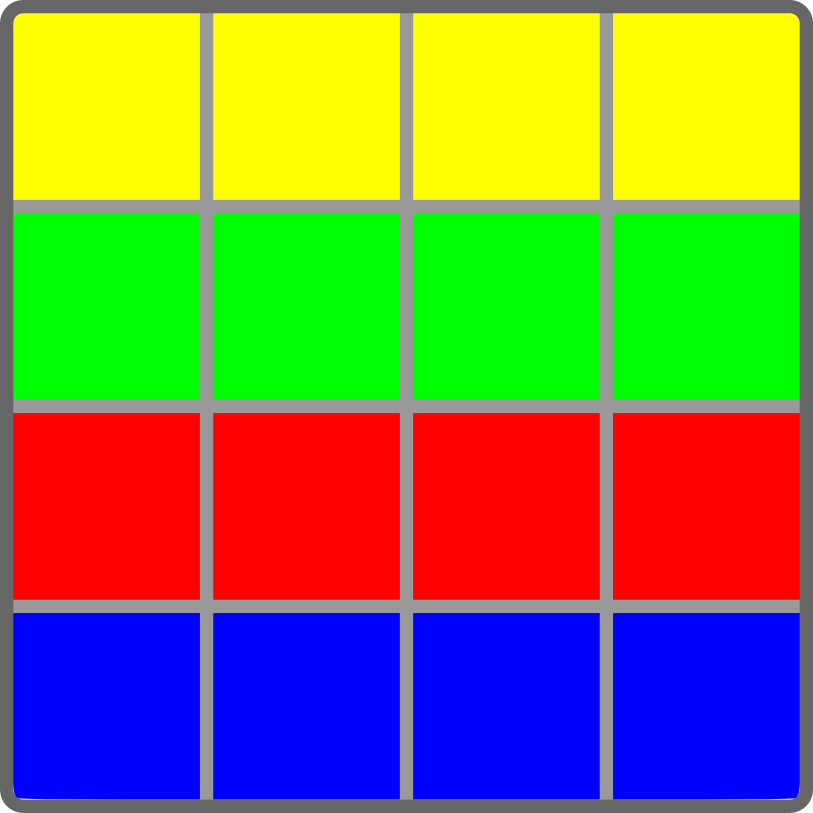
\includegraphics[width=0.55\textwidth]{images/rowPartitioning.png}
		\caption{Row partitioning}
		\label{fig:rowPartitioning}
	\end{subfigure}
	\begin{subfigure}{.3\linewidth}
		\centering
		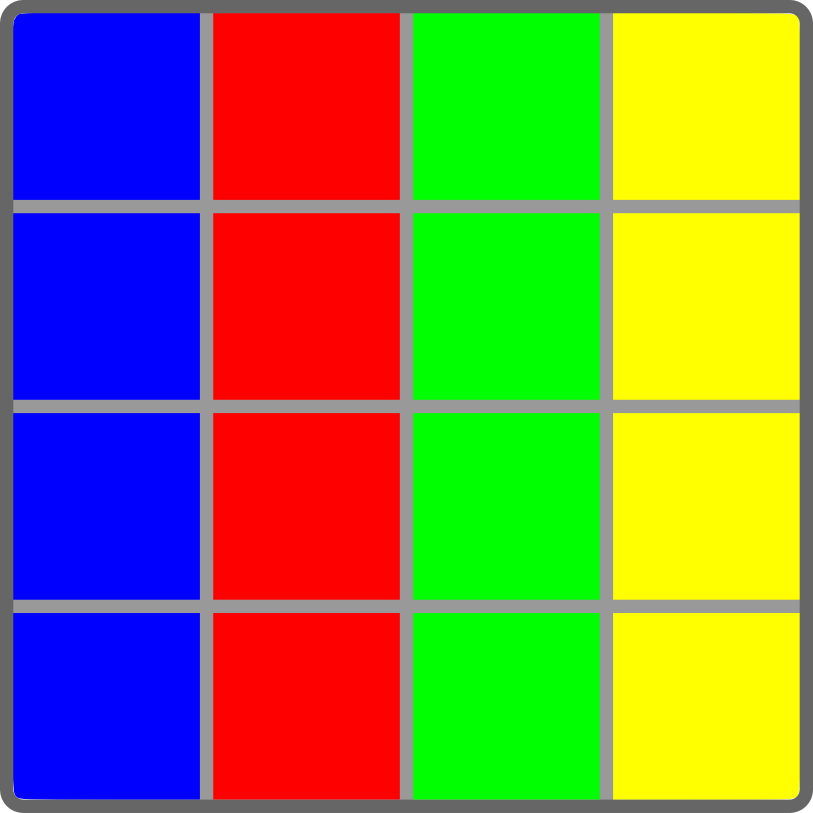
\includegraphics[width=0.55\textwidth]{images/columnPartitioning.png}
		\caption{Column partitioning}
		\label{fig:columnPartitioning}
	\end{subfigure}
	\begin{subfigure}{.3\linewidth}
		\centering
		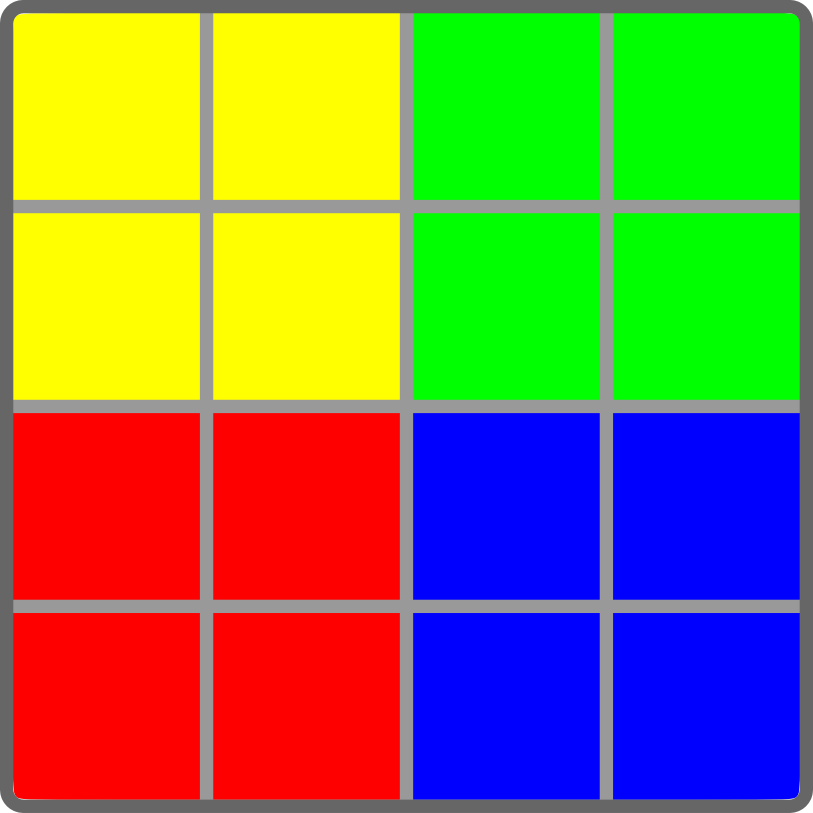
\includegraphics[width=0.55\textwidth]{images/quadraticBlockPartitioning.png}
		\caption{Quadratic block partitioning}
		\label{fig:quadraticBlockPartitioning}
	\end{subfigure}
	\caption{Row-wise, column-wise and quadratic block-wise matrix partitioning.}
	\label{fig:Partitionings}
\end{figure}

However, this approach unveils its drawbacks when multiplying two equally partitioned matrices $A$ and $B$ as illustrated in \cref{fig:rowPartitioningMM}.
In such a case, the row $r$ of $A$ and the complete matrix $B$ is needed to calculate the resulting row with index $r$.
This circumstance implies a complete repartitioning of $B$.
The repartitioning is especially grave, since $B$ has to be broadcasted to every row of $A$.

\begin{figure}[!h]
	\centering
	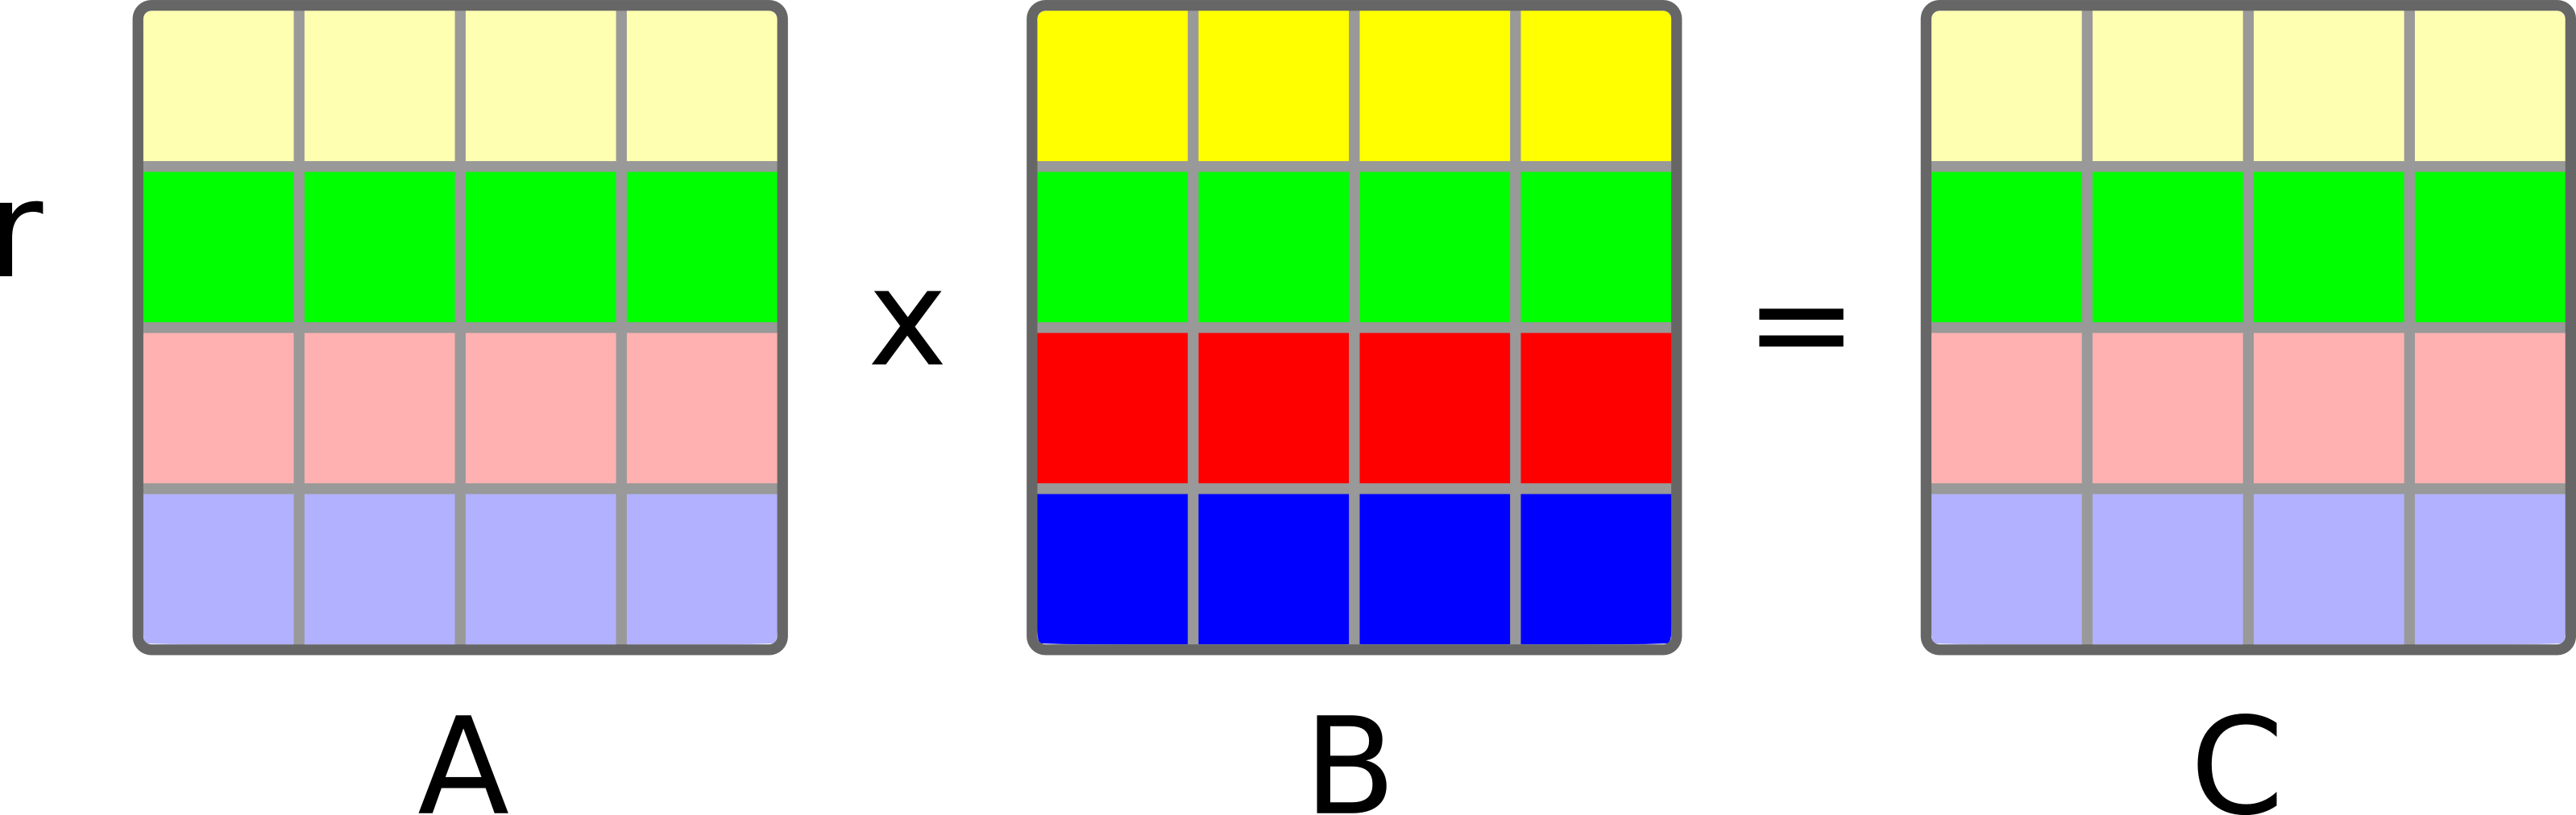
\includegraphics[width=0.6\linewidth]{images/rowMM.png}
	\caption{Matrix multiplication of $A$ and $B$. The required data to calculate row $r$ are highlighted.}
	\label{fig:rowPartitioningMM}
\end{figure}

In order to quantify the repartitioning costs of such a matrix multiplication, a simple cost model is developed.
First of all, it is limited to modeling the communication costs, since network I/O usually constitutes the bottleneck of distributed systems and is thus the dominating factor.
For the sake of simplicity, the multiplication of two quadratic matrices $A \in \mathbb{R}^{n\times n}$ and $B \in \mathbb{R}^{n\times n}$ giving the matrix $C\in \mathbb{R}^{n \times n}$ is considered.
Moreover, we assume that there are $n$ worker nodes available, each of which receiving a single row of $A$ and $B$, respectively.
Thus, $A$ and $B$ are row-wise partitioned.
We further assume that rows with the same index are kept on the same worker node.

Each row $a_r$ requires the complete knowledge of matrix $B$ in order to produce the row $c_r$.
Therefore, every row $b_r$ has to be sent to all other worker nodes.
Thus, the number of rows sent by each worker node is $n-1$.
All of the $n$ worker nodes have to do the same.
Consequently, the total number of sent messages is $n(n-1)$ and each message has a size of $n\alpha$ where $\alpha$ is the size of a matrix entry.
Usually, each sending operation causes some constant overhead inflicted by resource allocation.
Before sending the actual data over the network, memory to transfer the data to the network interface has to be allocated, network resources have to be reserved and a network connection with the remote peer has to be established.
This overhead is denoted by $\Delta$.
Since all sending operations occur in parallel, the costs caused by constant overhead are $(n-1)\Delta$.
The total amount of data, which has to sent over the network, is $n^2(n-1)\alpha$.
The network interconnection is assumed to guarantee every node a bandwidth $\nu$.
Therefore, the time needed for sending the data is $\frac{n^2(n-1)\alpha}{\nu}$.
These considerations lead to the following repartitioning cost model:

\begin{displaymath}
	cost_{row} = \frac{n^2(n-1)\alpha}{\nu} + (n-1)\Delta
\end{displaymath}

Row and column partitioning are extreme forms of blocking.
A less extreme form would be to split the matrix into equally sized quadratic blocks as shown in \cref{fig:quadraticBlockPartitioning}.
In order to identify the individual blocks, each of them will be assigned a block row and block column index assigned.
Thus, blocking adds some memory overhead in the form of index information.
An example of a $4\times 4$ matrix partitioned into $2\times 2$ blocks can be seen in \cref{fig:quadraticBlockPartitioningDetailed}.

\begin{figure}[!h]
	\centering
	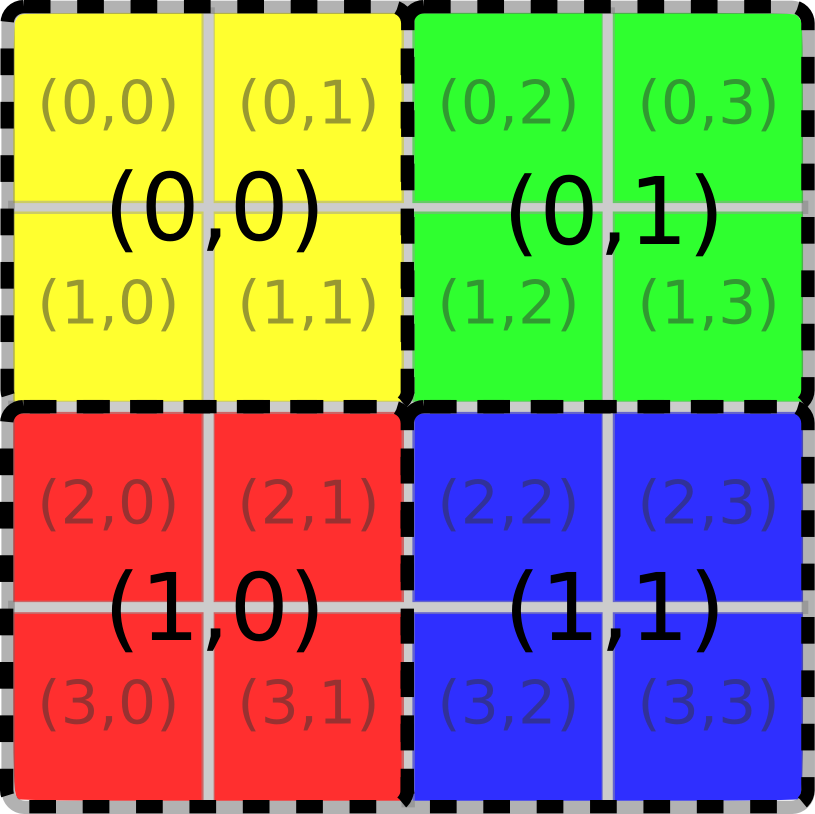
\includegraphics[width=0.25\linewidth]{images/quadraticBlockPartitioningDetailed.png}
	\caption{Detailed quadratic block partitioning with the added block row and block column indices.}
	\label{fig:quadraticBlockPartitioningDetailed}
\end{figure}

The blocks are distributed across the worker nodes.
The block size directly controls the granularity of the partitioning.
Increasing the block size will reduce the memory overhead of distributed matrices while reducing the degree of parallelism.
Thus, the user has to adjust the block size value depending on the matrix sizes and the number of available worker nodes in order to obtain best performance.

The quadratic block partitioning has similar properties like the row- and column-wise partitioning scheme when it comes to cellwise operations.
We simply have to join corresponding blocks with respect to the pair of block row and column index and execute the operation on matching blocks locally.
But how does this pattern performs for matrix multiplications?

The assumptions are the same as before and additionally it is assumed that $n$ is a square number.
Since the matrices $A$, $B$ and $C$ are equally partitioned into square blocks, indices will henceforth reference the block and not the matrix entry.
In order to calculate the block $c_{ij}$, we have to know the block row $a_{i}$ and the block column $b_{j}$.
The resulting block will be stored on the node $n_{ij}$ which already contains the blocks $a_{ij}$ and $b_{ij}$.
Thus, each node $n_{ij}$ has to receive the missing $2\left(\sqrt{n}-1\right)$ blocks from the block row $a_{i}$ and block column $b_{j}$.
In total, all worker nodes have to send $2n\left(\sqrt{n}-1\right)$ blocks.
Each block has the size $n\alpha$.
The total communication costs comprises the transmission costs and the network overhead:

\begin{displaymath}
	cost_{squareBlock} = \frac{2n^2\left(\sqrt{n}-1\right)\alpha}{\nu} + 2\left(\sqrt{n}-1\right)\Delta
\end{displaymath}

We see that the term $(n-1)$ is replaced by $2\left(\sqrt{n}-1\right)$ in the square block cost model.
For $n>2$, the square block partitioning scheme is thus superior to the row- and column-wise partitioning pattern with respect to the cost model.
The reason for this outcome is that the square blocks promote more localized computations compared to the other partitionings.
Instead of having to know the complete matrix $B$, we only have to know one block row of $A$ and one block column of $B$ to compute the final result.

Due to these advantages and also considering its simplicity, we decide to implement the square block partitioning scheme in Gilbert.
It would also be possible to combine different partitionings and select them dynamically based on the data sizes and input partitionings.

Besides the partitioning, Gilbert also has to represent the individual matrix blocks.
There exist several storing schemes for matrices depending on the sparsity of the matrix.
For example, if a matrix is dense, meaning that it does not contain many zero elements, the elements are best stored in a continuous array.
If a matrix is sparse, then a hash map or some form of compressed representation are best suited.
Gilbert chooses the representation of each block dynamically.
Depending on the non-zero elements to total elements ratio, a sparse or dense representation is selected.

\subsection{Linear Algebra Operations}
\label{sec:LinearAlgebraOperations}

The other aspect of writing distributed algorithms is to think about how the algorithms work with the locally available data and which data has to be communicated in order to compute the final result.
Stratosphere and Spark both offer a highly expressive programming API, which follows and extends the well-known MapReduce paradigm~\cite{dean:c2008a}.
Conceptually, a set of distributed data items, called \emph{DataSet} or \emph{RDD} (resilient distributed dataset) in the context of Stratosphere and Spark, respectively, forms the basis of both systems.
There are several ways to initially create a data set, such as reading from a file or distribution of a local collection.
Once a distributed data set is created, it can be modified by applying one of the transforming functions, namely \emph{map}, \emph{reduce}, \emph{join}, \emph{cross} or \emph{coGroup}.
These functions are borrowed from the world of functional programming, since they happen to be expressive enough and can serve as a utile abstraction for automatic parallelization.
Each of these transforming functions takes one or more data sets as inputs and produces a new distributed data set.
The distributed data sets are not computed directly but instead they generate a dataflow plan which is lazily executed later on.
Each node of the dataflow plan constitutes a function application and consequently a new data set.
The edges connect input data sets to output data sets and thus represent the data dependencies.

In order to understand how the different linear algebra operations are implemented, we will quickly revise the semantics of the transforming functions.
For a more detailed explanation, the reader is referred to~\cite{zaharia:2012a,alexandrov:2011a,battre:2010a}.
A distributed data set is a multiset of items.
An item can have a key value, which is retrieved by the $key$ function.
Each of the transforming functions is called with a user defined function (UDF), which specifies how each item is processed and what kind of item is emitted as the result.
In other words, it defines the program specific semantics of the transformation.

\begin{description}
	\item[map] The map operator is called with one input data set $A$ and a UDF. The UDF is called for each item $a\in A$ independently, producing one result item.

	\item[reduce] The reduce operator partitions the input data set $A$ into groups of items with the same key. 
		All items of each group are handed together to a call of the UDF.
		In other words, the UDF is called for each submultiset $A^\prime$ with $\forall a,b\in A^\prime : key(a) = key(b)$ and $\forall a \in A^\prime, b\in A \setminus A^\prime: key(a) \not = key(b)$.

	\item[join] The join operator joins two data sets $A$ and $B$ with respect to a key value.
		This means that a UDF is called for each pair $(a,b)$ with $a\in A$ and $b\in B$ with $key(a)=key(b)$.

	\item[cross]The cross operator can be understood as the Cartesian product.
		Given two data sets $A$ and $B$, cross calls the UDF for each pair $(a,b)$ with $a\in A$ and $b\in B$.
	\item[coGroup] The coGroup operator also takes 2 input data sets $A$ and $B$.
		It groups the elements of $A$ and $B$ according to their keys and joins the grouped submultisets.
		In other words, the UDF is called for each pair of multisets $(A^\prime, B^\prime)$ with $A^\prime \subseteq A \wedge B^\prime \subseteq B \wedge |keyset(A^\prime \cup B^\prime)| = 1$ and $keyset(A^\prime \cup B^\prime) \cap keyset((A \cup B) \setminus (A^\prime \cup B^\prime)) = \emptyset$.
		The function $keyset$ is the set of appearing keys in a set: $keyset(X) \coloneqq \{ key(x) \mid x \in X \}$.
\end{description}

Stratosphere as well as Spark offer a similar set of second-order functions comprising the abovementioned functions.
Consequently, we can develop the linear algebra operations in a general fashion and do not have to adhere to a specific framework.
In the following, we will outline the implementation behind the different intermediate operators with respect to the transforming functions.
We assume that the matrices are partitioned using the square block scheme.

The \code{ScalarMatrixTransformation} and \code{MatrixScalarTransformation} work on a matrix input and a scalar input.
The scalar input is a distributed data set with one item.
The scalar value is required at every matrix block to perform the \code{smOp} operation.
Thus, we use the cross function to pair the scalar value with every matrix block.
The resulting dataflow plan is shown in \cref{fig:planScalarMatrixTransformation}.

\begin{figure}[!h]
	\centering
	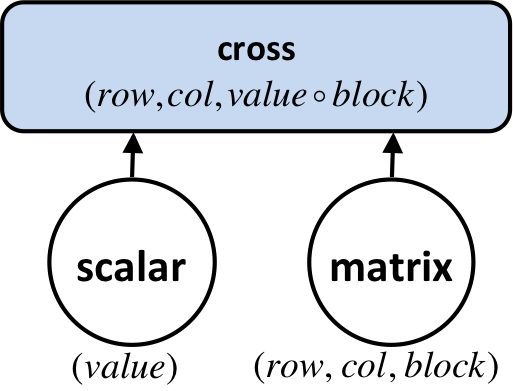
\includegraphics[width=0.25\linewidth]{images/planScalarMatrixTransformation.png}
	\caption{Dataflow plan of the \code{ScalarMatrixTransformation}.}
	\label{fig:planScalarMatrixTransformation}
\end{figure}

The \code{CellwiseMatrixTransformation} operates locally on the cells of a single matrix.
Thus, no communication is needed and the \code{unaryScalarOp} operation $f$ can be executed embarrassingly parallel.
The transformation is implemented using the map function.
The resulting dataflow plan is shown in \cref{fig:planCellwiseMatrixTransformation}.

\begin{figure}[!h]
	\centering
	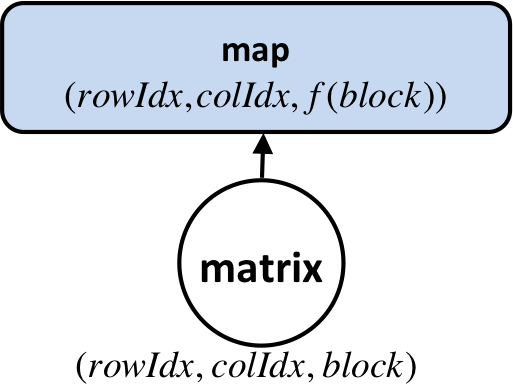
\includegraphics[width=0.25\linewidth]{images/planCellwiseMatrixTransformation.png}
	\caption{Dataflow plan of the \code{CellwiseMatrixTransformation}.}
	\label{fig:planCellwiseMatrixTransformation}
\end{figure}

The \code{CellwiseMatrixMatrixTransformation} operates locally on the cells of two matrices.
It applies an operation of type \code{scalarOp} to each pair of corresponding cell entries.
Therefore, we have to pair all matrix blocks which have the same block row and block column index.
Assuming, $f$ is the function performing the cellwise operation on the given matrix blocks, the resulting dataflow plan can be seen in \cref{fig:planCellwiseMatrixMatrixTransformation}.
The join function is represented as a join and a map node in the dataflow plan.
The map function is called for each of the matching pairs created by the join node.

\begin{figure}[!h]
	\centering
	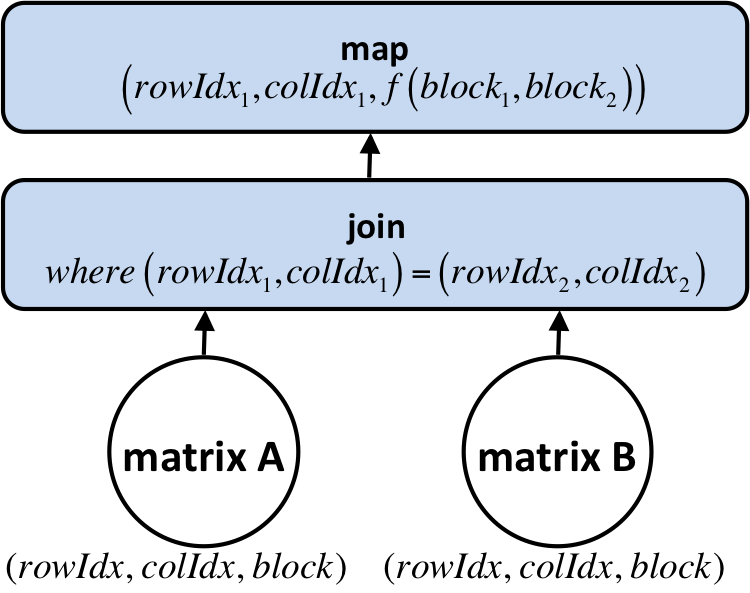
\includegraphics[width=0.365\linewidth]{images/planCellwiseMatrixMatrixTransformation.png}
	\caption{Dataflow plan of the \code{CellwiseMatrixMatrixTransformation}.}
	\label{fig:planCellwiseMatrixMatrixTransformation}
\end{figure}

Matrix multiplications are probably the most critical operation for performance in linear algebra programs.
Therefore, we have to pay attention to a thorough implementation within Gilbert.
In a MapReduce-like system there exist two distinct matrix multiplication implementations for square blocking.
The first approach is based on replicating rows and columns of the operands and is called replication based matrix multiplication (RMM).
The other method is derived from the outer product formulation of matrix multiplications.
It is called cross product based matrix multiplication (CPMM).
The RMM and CPMM methods have been implemented within SystemML~\cite{ghoting:2011a}.

Let us assume that we want to calculate $A \times B = C$ with $A,B$ and $C$ being matrices.
The block size has been chosen such that $A$ is partitioned into $m\times l$ blocks, $B$ is partitioned into $l \times n$ blocks and the result matrix $C$ will be partitioned into $m\times n$ blocks.
In order to reference the block in the $i$th block row and $j$th block column of $A$, we will write $A_{ij}$.
A block row will be denoted by a single subscript index and a block column by a single superscript index.
For example, $A_i$ marks the $i$th block row of $A$ and $A^j$ the $j$th block column of $A$.

The replication-based strategy will copy for each $C_{ij}$ the $i$th block row of $A$ and the $j$th block column of $B$.
The replicated blocks of $A_i$ and $B^j$ will be grouped together.
These steps can be achieved by a single mapper.
Once this grouping is done, the final result $C_{ij}$ can be calculated with a single reducer.
The reduce function simply has to calculate the scalar product of $A_i$ and $B^j$.
It is important to stress that $A_i$ is replicated for each $C_{ik},\forall k$.
The whole process is illustrated in \cref{fig:RMM}.

\begin{figure}[!h]
	\centering
	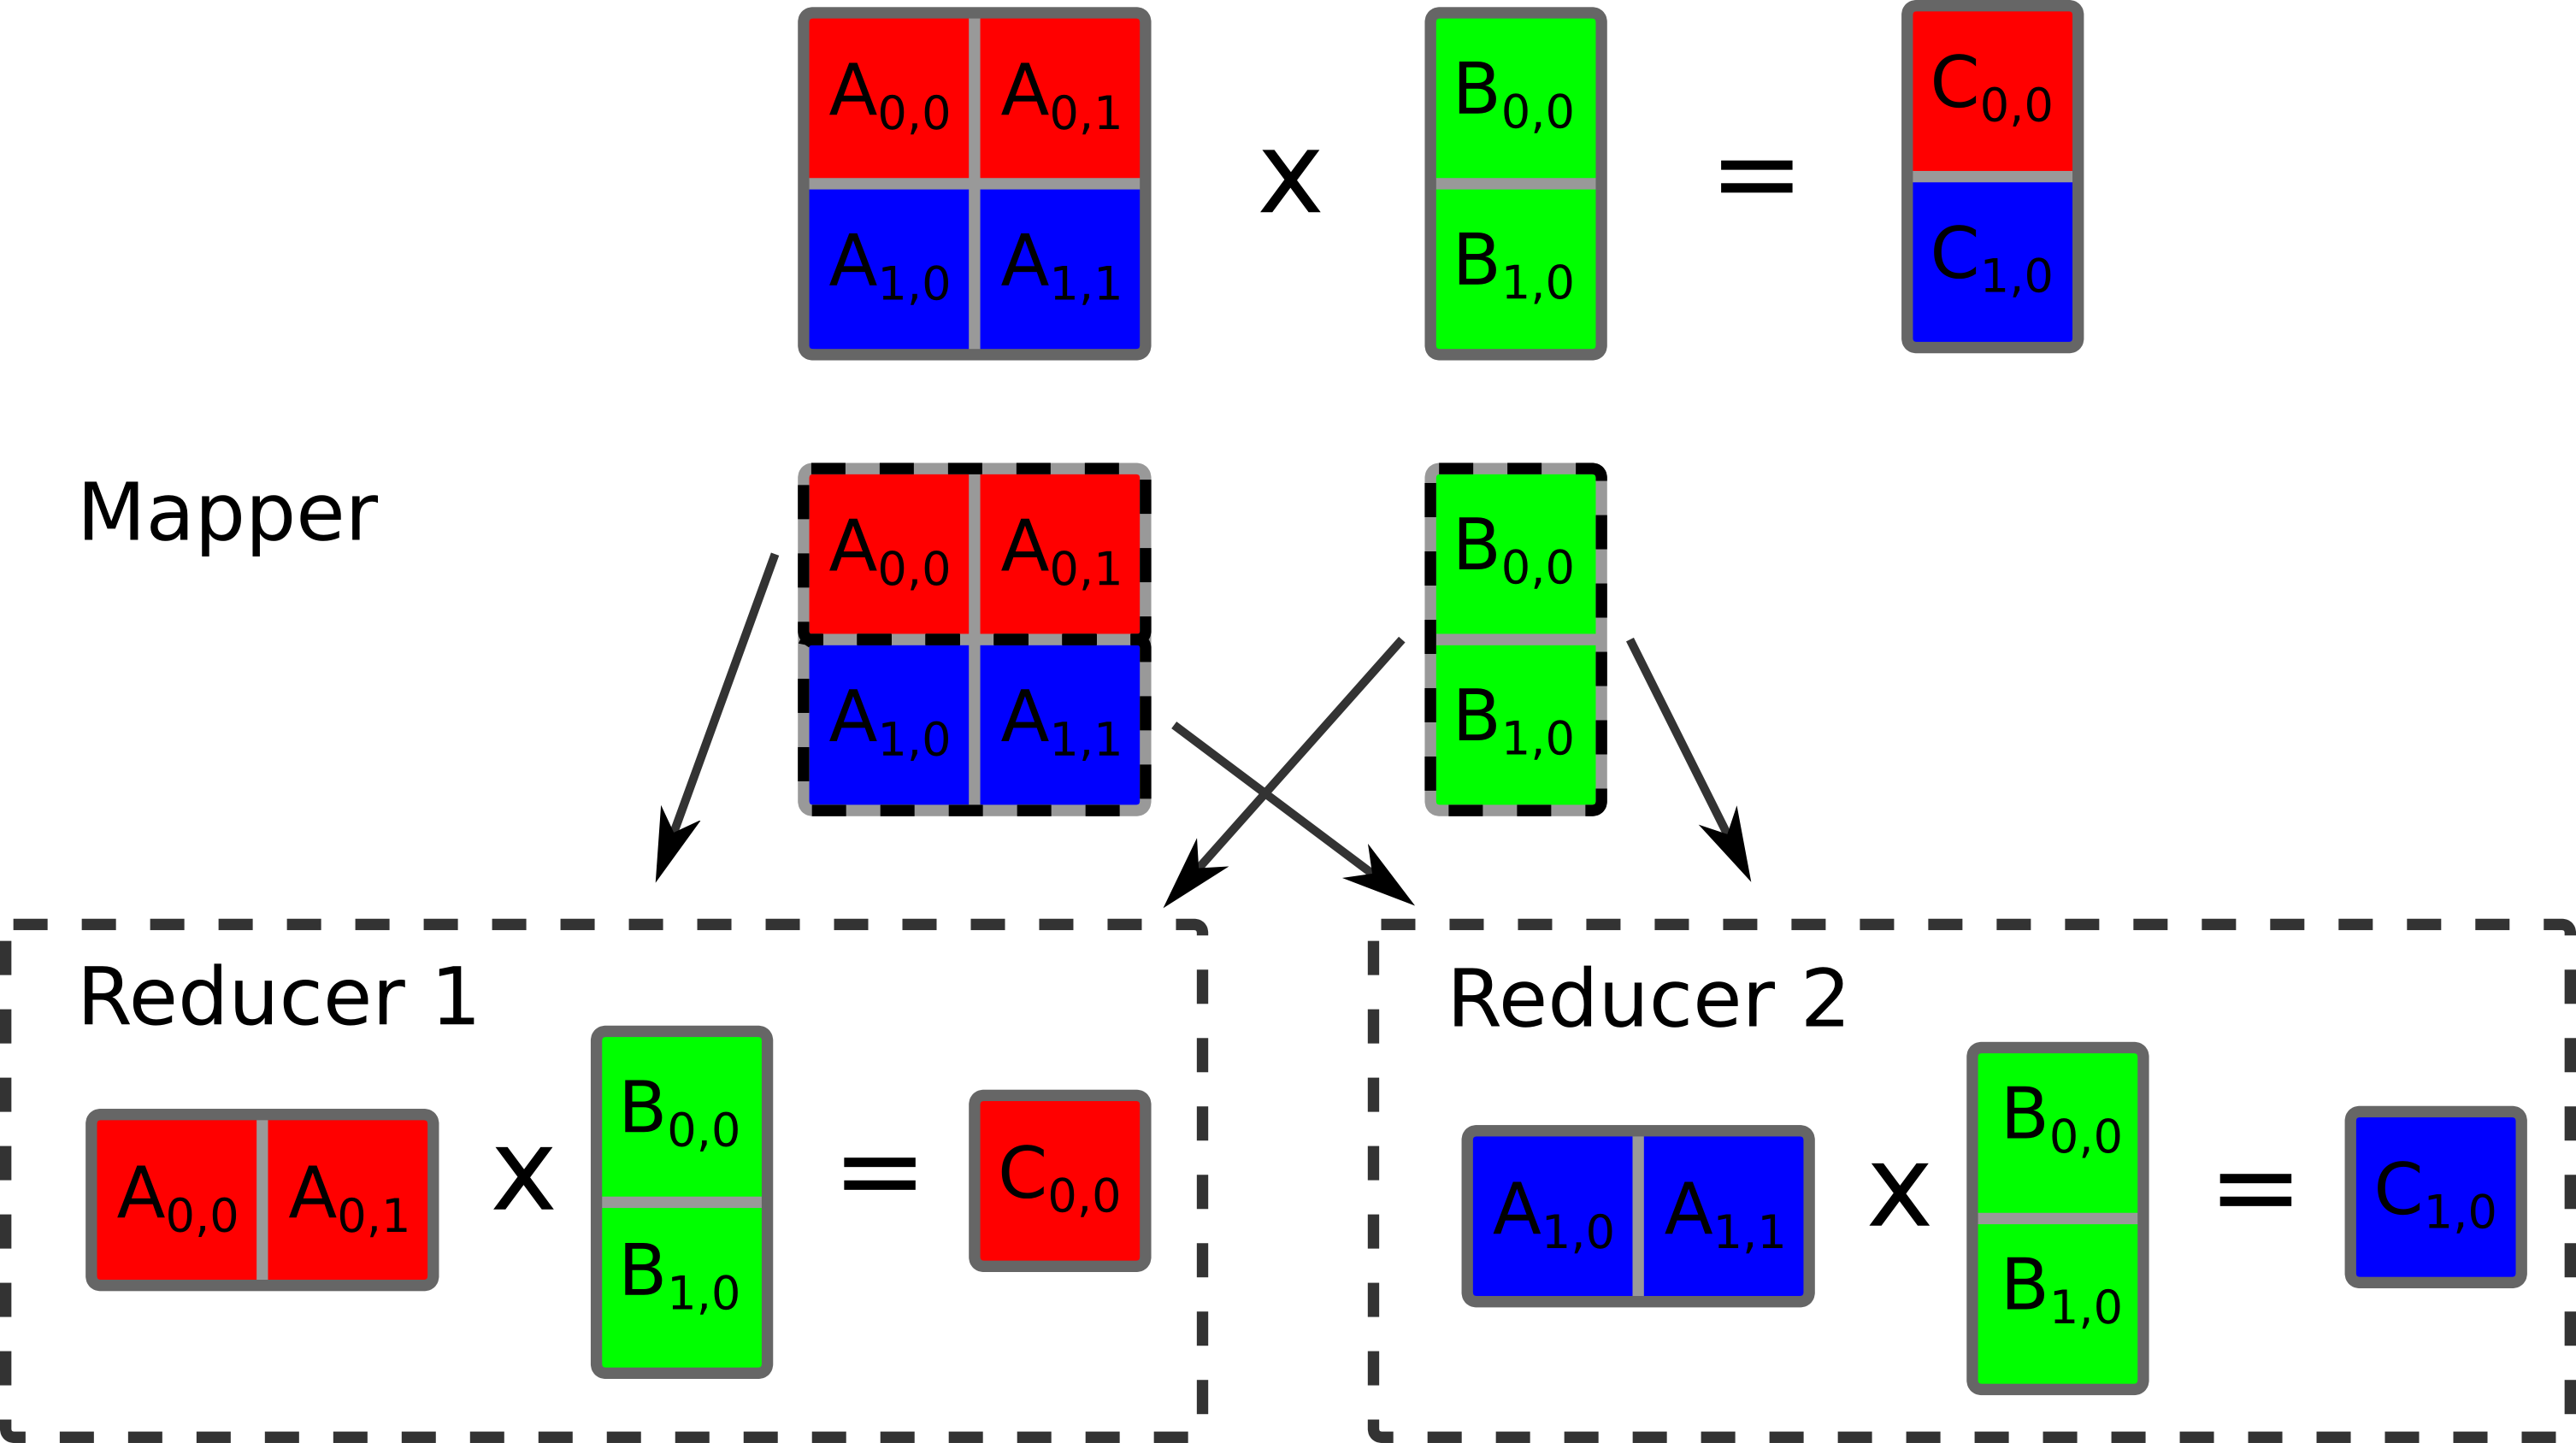
\includegraphics[width=0.4777\linewidth]{images/rmm.png}
	\caption{Replication based matrix multiplication with MapReduce.}
	\label{fig:RMM}
\end{figure}

In contrast to RMM, CPMM calculates the outer products between $A^k$ and $B_k$ for all $k$.
A mapper can group the $A^k$ and $B_k$ together so that a reducer can compute the outer products.
Consequently, this method does not replicate any data.
The outer product produces intermediate result matrices $C^k$ which have to be added up to produce the final result $C=\sum_{k=1}^{l} C^k$.
This summation can be achieved by a subsequent reducer.
The whole process is illustrated in \cref{fig:CPMM}.

\begin{figure}[!h]
	\centering
	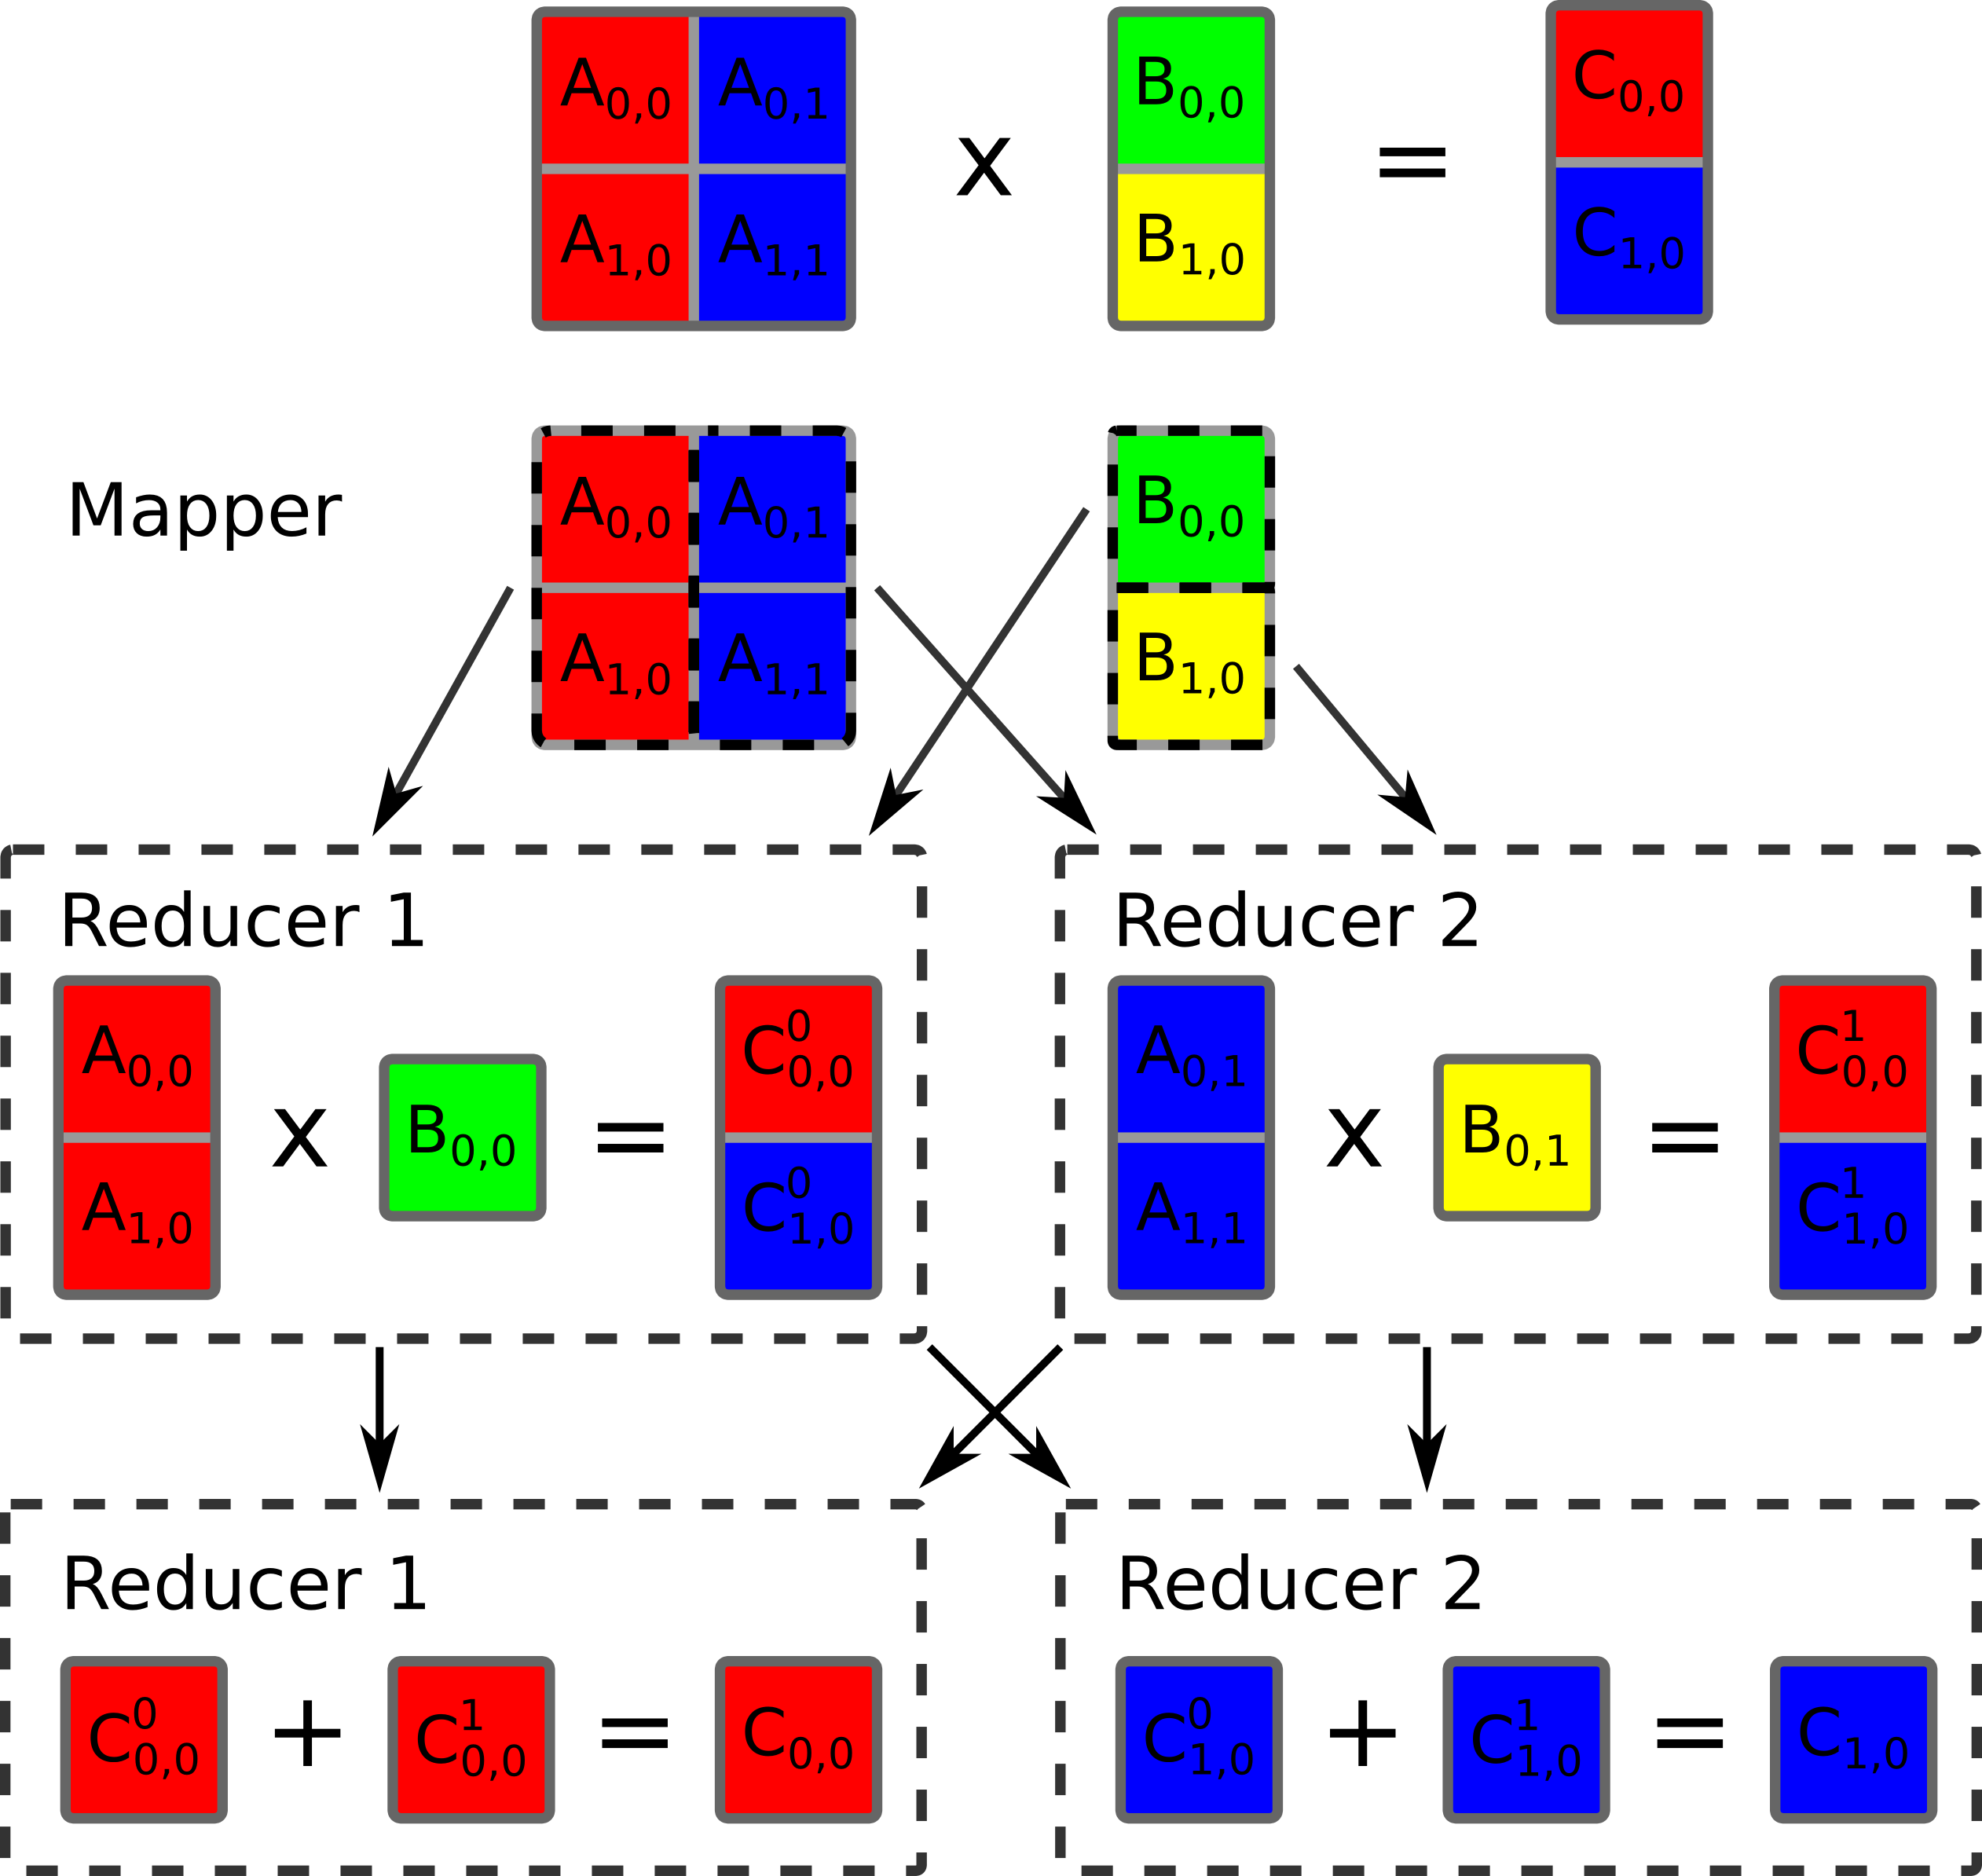
\includegraphics[width=0.4\linewidth]{images/cpmm.png}
	\caption{Cross product matrix multiplication with MapReduce.}
	\label{fig:CPMM}
\end{figure}

The methods RMM and CPMM differ in terms of network communication.
The former method can be realized within a single MapReduce job whereas the latter requires two.
Neither RMM nor CPMM is always superior.
The optimal matrix multiplication strategy depends on the matrix size of its operands $A$ and $B$.

Fortunately, Stratosphere and Spark exhibit a little bit more flexibility in terms of higher order functions.
Freed from the tight corset of the MapReduce world, matrix multiplications can be expressed more subtly.
Looking at the definition of the matrix multiplication for $C_{ij}=\sum_{k=1}^{l}A_{ik}\times B_{kj}$, it can be seen that every $A_{ik}$ has to be joined with its corresponding $B_{kj},\forall k$.
This pairwise mapping can be easily achieved by using the join function.
The join-key is the column index of $A$ and the row index of $B$.
The joiner calculates for each matching pair $A_{ik}$ and $B_{kj}$ an intermediate result $C_{ij}^k$.
Grouping the intermediate results with respect to the index pair $(i,j)$ allows us to compute the final result in a subsequent reduce step.
The overall algorithm strongly resembles the CPMM.
The corresponding dataflow plan is shown in \cref{fig:planMatrixMultiplication}.

\begin{figure}[!h]
	\centering
	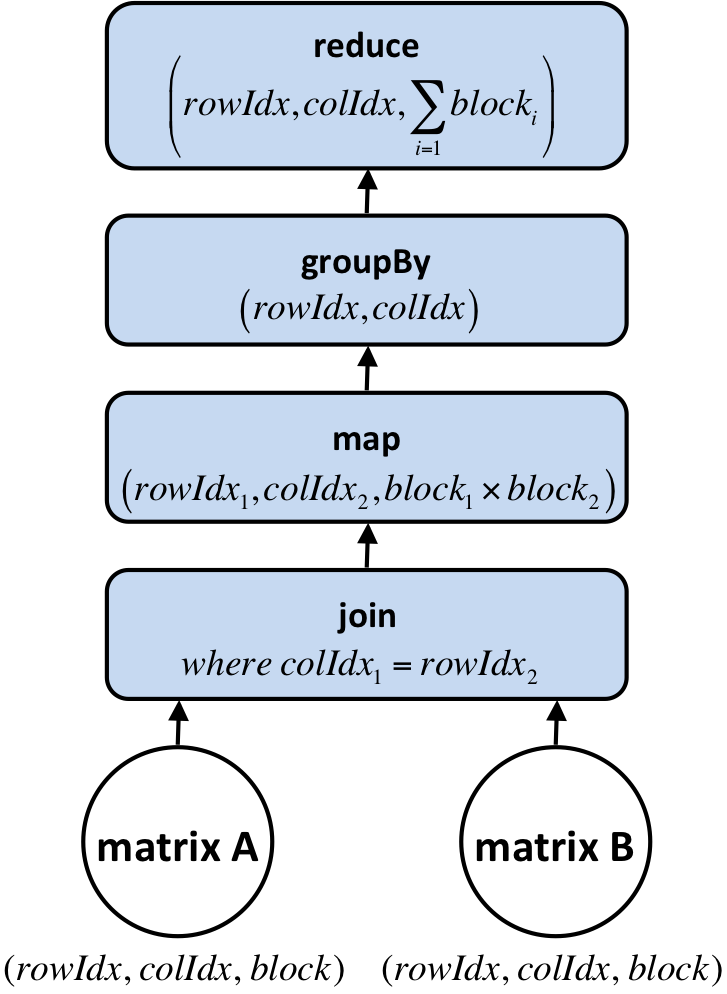
\includegraphics[width=0.354\linewidth]{images/planMatrixMultiplication.png}
	\caption{Dataflow plan of the \code{MatrixMult} operator.}
	\label{fig:planMatrixMultiplication}
\end{figure}

Stratosphere supports several execution strategies for the higher-order functions.
A cost-based optimizer selects the best strategies prior to execution.
One possible optimization concerns the join function.
The join can either be realized using a hybrid-hash join or a sort-merge join algorithm depending on the current partitioning and the input data sizes.

If one input data is relatively small compared to the other input, it is usually more efficient to use the hybrid-hash join algorithm.
Without loss of generality, we assume that the matrix $B$ constitutes such a small input.
If we further assume that the block rows of $A$ are kept on the same worker node, then the last reduce operation can be executed locally and without any shuffling.
The resulting execution plan under these assumptions is equivalent to the RMM.

If the system chooses the sort-merge join algorithm instead, then the columns of $A$ will be distributed across the worker nodes.
Consequently, the last reduce step causes a mandatory repartitioning.
Then, the resulting execution plan is equivalent to the CPMM.

Even though Gilbert has only one dataflow plan specified to implement the matrix multiplication, the Stratosphere system can choose internally between the RMM and CPMM strategy.
The strategy is selected by the optimizer which bases its decision on the data size and the partitioning, if available.
Consequently, Stratosphere frees the programmer from this decision.

The \code{VectorwiseMatrixTransformation} operator cannot be generalized independently of the \code{vectorwiseOp} operation.
For example, consider the maximum and the norm operation.
The maximum is calculated by taking the maximum of each row in a block.
Afterwards, the maximum per block is grouped with respect to the block row index and the grouped blocks are reduced by taking the maximum over all group elements.
Grouping is based on the key of each item.
The corresponding dataflow plan is shown in \cref{fig:planMaximumVectorwiseTransformation}.

\begin{figure}[!h]
	\centering
	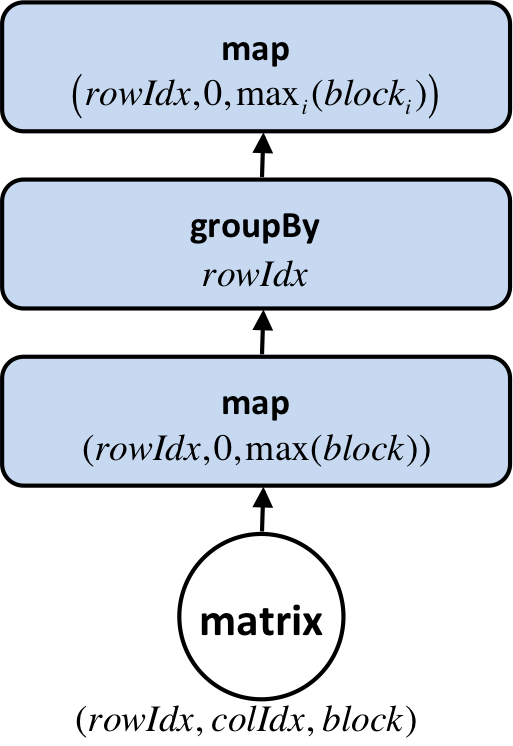
\includegraphics[width=0.25\linewidth]{images/planMaximumVectorwiseTransformation.png}
	\caption{Dataflow plan of the \code{VectorwiseMatrixTransformation} with the \code{max} operation.}
	\label{fig:planMaximumVectorwiseTransformation}
\end{figure}

In contrast to that, the $2$-norm operation requires a more sophisticated implementation.
First, the cellwise square of all matrix entries is calculated with the map function.
Then, the partial sums of every row are computed by summing the columns of each block.
This calculation constitutes another map operation.
The final row sums are calculated by grouping the partial sums with respect to their block row index and summing the items of each group up.
After this reduce operation is done, the final result is computed by taking the cellwise square root.

The \code{AggregateMatrixTransformation} operator computes an aggregate over all elements of the matrix.
Given that the aggregate operation is combinable, meaning that the aggregation can be expressed as a fold operation in terms of functional programming, we can implement it straightforwardly.
We only need a reducer with the aggregation function $f$ as UDF.
The respective dataflow plan can be found in \cref{fig:planAggregateMatrixTransformation}.
The $default$ variable holds the initial value for the fold operation.
In case that the aggregate is not combinable, it has to be implemented individually.

\begin{figure}[!h]
	\centering
	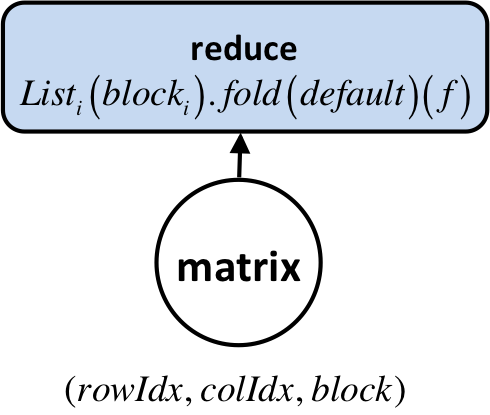
\includegraphics[width=0.25\linewidth]{images/planAggregateMatrixTransformation.png}
	\caption{Dataflow plan of the \code{AggregateMatrixTransformation}.}
	\label{fig:planAggregateMatrixTransformation}
\end{figure}
%!TEX root=main.tex
\section{Architecture}
\label{cha:architecture}

Gilbert provides a Matlab-like language for distributed sparse linear algebra operations.
Being such a system, it comprises the complete stack of functionalities necessary to implement a programming language.
At first, the system has to divide the given source code into tokens.
These tokens are parsed and an abstract syntax tree (AST) is created.
In order to generate the intermediate representation (IR), it is necessary to assign types to the occurring expressions.
This assignment is done by the typing system.
Afterwards, the compiler can translate the Gilbert program into its IR.
The IR is well suited to apply high-level transformations to the program.
At last, the execution plan generator translates the IR into an execution plan which can be executed in parallel.

Since we had to implement the whole stack of functionalities of a programming language, Gilbert became quite complex.
In order to control this complexity, Gilbert's functionalities were separated into different layers with distinct tasks.
The layered system architecture is shown in \cref{fig:systemArchitecture}.
The separation of concerns limits the complexity of each layer so that each one of them becomes manageable.
In cooperation, though, they implement a highly elaborate system.

\begin{figure}
	\centering
	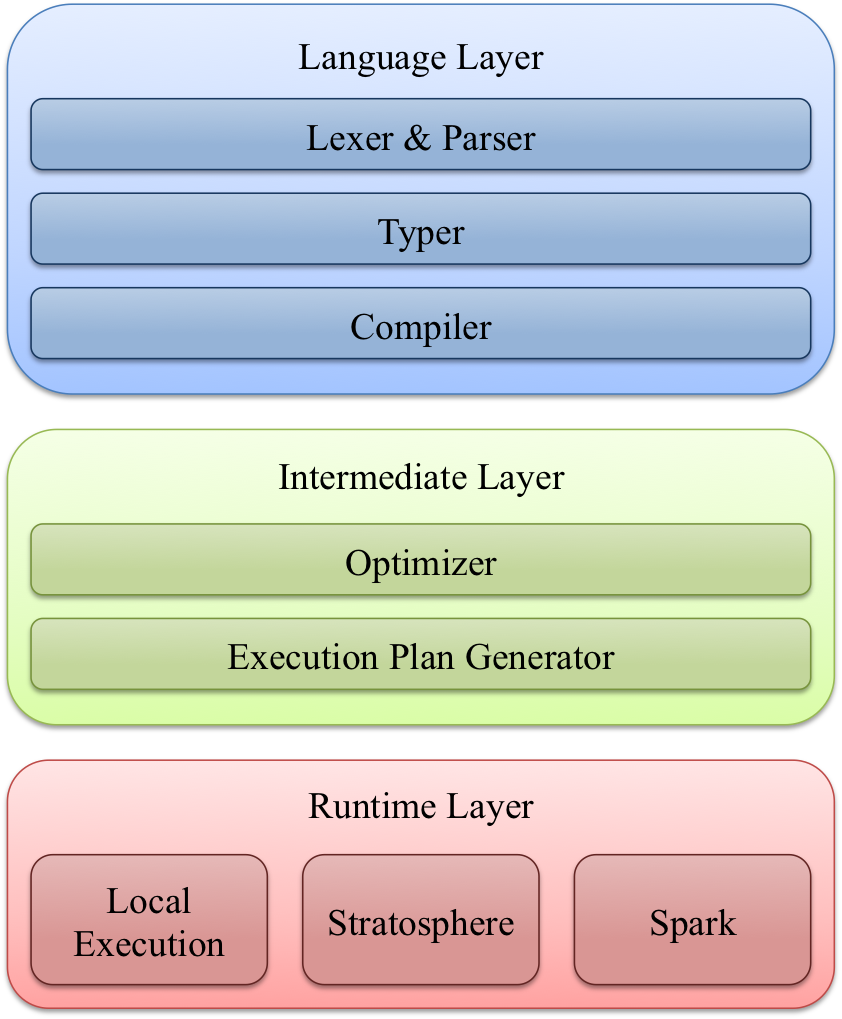
\includegraphics[width=0.5\linewidth]{images/systemArchitecture.png}
	\caption{The layered system architecture of Gilbert. The language layer is responsible for parsing, typing and compiling the given Matlab code. The intermediate layer facilitates high-level optimization strategies. The runtime layer is responsible for executing the specified program in parallel.}
	\label{fig:systemArchitecture}
\end{figure}

The first layer is the language layer.
It contains all functionality to parse the given Gilbert code and to compile it into the IR.
The second layer is the intermediate layer and it receives the IR of the Gilbert code.
The intermediate format is the ideal representation to apply language independent high-level transformations.
Consequently, the second layer hosts the optimizer.
The Gilbert optimizer applies several algebraic optimizations prior to the generation of the execution plan.
The execution plan generator translates the optimized IR into a specific execution plan, depending on the selected execution engine.
Once the program has been translated into an execution engine's specific plan, it is executed on the respective back end.

\subsection{Language Layer}

The language layer contains all the logic for translating Gilbert source code into the intermediate representation, see \cref{cha:intermediaterepresentation} for more details.
The layer itself is subdivided into three layers.
The first of these sublayers is the lexer and parser of MATLAB code.
Gilbert uses a recursive descent parser with backtracking, which is capable of parsing any LL(*) grammar.
Consequently, it can also parse Gilbert's front end language as specified in \cref{sec:languageGrammar}.

Once the MATLAB code is parsed, it is given to the next layer, namely the typing layer.
Here, the produced AST is attributed with type information.
This information is inferred automatically from the source code without any need for explicit type annotations.
The typer makes use of the Hindley-Milner type inference system, as it is described in \cref{sec:hmInference}.
After the types have been inferred, a new AST with additional type information is generated.

The type information enriched AST is given to the last sublayer.
The compiler is responsible for translating the AST into a front end independent representation of linear algebra operations, namely the IR.
The format Gilbert uses to represent linear algebra operations in a generalized format is described in \cref{cha:intermediaterepresentation}.
In fact, it is also some form of AST just without the peculiarities of MATLAB.

\subsection{Intermediate Layer}

The intermediate layer contains the optimizer and the execution plan generator.
The optimizer works on the intermediate representation of the Gilbert program.
It applies the optimizations described in \cref{cha:optimizer}.
The execution plan generator's task is to translate the intermediate format into the execution engine's specific format.
Currently, the system supports local execution and two engines for distributed execution, namely Stratosphere and Spark.

For the local execution, Gilbert employs an interpreter.
The interpreter directly executes the intermediate representation.
Beginning at the root of the dependency tree, the interpreter utilizes a recursive-descent strategy to evaluate each node.
In order to evaluate a given node of the tree, the interpreter first descends to its children.
After having retrieved the results of the children nodes, the parent node is evaluated.

The distributed execution engines do not support immediate execution of the individual nodes.
Instead, the plan generator has to create an execution plan for Stratosphere and Spark, which is lazily executed upon submission or when Spark's actions are called.
Fortunately, Stratosphere and Spark offer a similar programming API.
Thus, Gilbert can translate the distinct linear algebra operations using the same general building blocks as described in \cref{sec:LinearAlgebraOperations}.
The execution plan is generated using a recursive-descent approach similar to the local interpreter.
Once the intermediate representation has been transformed, the plan is sent to the respective system.
The system is responsible for the parallel execution.

\subsection{Runtime Layer}

The runtime layer marks the transition from Gilbert to one of the supported execution engines.
It is more of a conceptual abstraction of the Gilbert system.
Gilbert supports 3 different engines at the moment, but it should be easy to add support for further execution systems.

%!TEX root=main.tex
\section{Implementation}
\label{cha:implementation}

The development of Gilbert involved the implementation of the complete technology stack of a programming language.
For each technology, we had to decide how to implement it.
The lexer and parser, for example, can be automatically generated using tools such as ANTLR~\cite{antlr}, Bison~\cite{bison} or Yacc~\cite{yacc}.
However, using these tools would have required to manage the complexity of several frameworks and probably a lot of boilerplate code to fuse them together.
Therefore, we looked for a tool with the potential to implement the complete stack of Gilbert.

Fortunately, the Scala language~\cite{scala,odersky:2010a} unifies all required technologies under one umbrella.
Scala is a highly scalable language, well suited for script sized programs as well as enterprise applications.
The language combines object oriented and functional programming, giving a maximum of flexibility to the programmer.
The Scala code is compiled to Java bytecode and thus executed on a JVM.
This feature makes the language platform independent to the greatest possible extent.
Furthermore, it can integrate existing Java code and thus benefit from the rich set of Java libraries.
Last but not least, it is like the new cool kid on the block of programming languages, which everyone likes.

An important aspect of our choice was how easily a parser and a compiler can be implemented with Scala.
If one decides to implement these programs within a popular language such as Java, C/C++ or C\# and without any additional tools, then it quickly becomes a tedious and error-prone task.
That's the reason why tools like Yacc and ANTLR have emerged.
Scala circumvents this problem by providing an internal domain specific language (DSL) for an easy and quick development of parsers and lexers.
This DSL is also known as Scala Parser Combinators.
Once an abstract syntax tree has been generated using these parser combinators, it is very easy to develop a compiler using Scala's pattern matching functionality.
The pattern matching capabilities of Scala are similar to functional languages, such as Haskell, ML or OCaml.
It can even be applied on object hierarchies, making it a powerful tool for OOP and functional programming likewise.
The Scala Parser Combinators generate recursive descent parsers which are capable of parsing LL(*) grammars.

We decide to develop Gilbert as an open source project so that everyone can benefit from the project.
The complete source code is hosted on Github and is publicly accessible under \url{https://github.com/gilbert-lang/gilbert}.

\subsection{Math-Backend}
\label{sec:mathBackend}

In \cref{cha:gilbertruntime} we have explained the representation of distributed matrices and how the intermediate operators are mapped to dataflow plans.
What was left out, though, is how the local operations on the block-level are implemented.
Consider, for example, the matrix multiplication of two distributed matrices.
The result is obtained by joining the blocks of both operands, performing a local matrix multiplication on a matching block pair and reducing the intermediate results.
The local matrix multiplication is self-contained and has to be executed by some algorithm.
Since there already exist highly optimized algorithms for different matrix representations, dense or sparse, we do not have to reinvent the wheel.

One of the numerous linear algebra libraries for the Java ecosystem is Mahout~\cite{mahout:2011a}.
The math library of Mahout is mainly written in Java and thus offers a Java binding.
Initially, Mahout was used to implement the local linear algebra operations of Gilbert.
However, it quickly turned out that Mahout lacked reliable support for sparse matrices and suffered from poor performance.
Since Gilbert is geared towards being a linear algebra environment for sparse matrices with descent performance, we were forced to look for alternatives.
Next we came across Breeze~\cite{breeze}, a library for numerical processing written in Scala.

Breeze offers data structures for all linear algebra primitives, such as matrices and vectors.
Additionally, it supports sparse and dense variants.
For each version, Breeze is shipped with elaborate algorithms implementing the linear algebra operations.
In case that the host has a BLAS or LAPACK library installed, which is compiled and optimized for the underlying architecture, Breeze automatically detects and uses it.
That way, Breeze can achieve near optimal performance when multiplying dense matrices compared to compiled languages such as C/C++ and Fortran.
Under the hood, Breeze relies on the netlib-java library for this feature.
The fact that it offers a Scala binding allowed it to be integrated seamlessly into Gilbert.
We have chosen this library as our principal math back end because it is clean, very reliable and extremely powerful.

Additionally, Gilbert also supports the aforementioned Mahout library as a secondary math back end.
The user can select on demand which system he wants to use depending on his personal preference.
The inclusion of Mahout also emphasizes the extensible architecture of Gilbert.
It is very easy to add further math libraries to Gilbert.

\subsection{Execution Engines}

From the very first moment, Gilbert was intended as a general purpose linear algebra front end for different runtime systems.
Therefore, Gilbert includes an abstraction, called execution engine, which encapsulates the logic for running a Gilbert program.
Currently, Gilbert comes with three different execution engines.
The local executor serves as a reference implementation of the linear algebra operations and can be used for computing little data on a single machine.
But the purpose of Gilbert was to enable linear algebra programs to handle big data and thus a distributed execution is strictly necessary.
The Stratosphere and Spark executor fulfill that condition.
However, Gilbert is not restricted to these systems as backends.
In fact, it should be easy to add new execution engines to Gilbert.
They only have to be able to map the intermediate operators to their runtime specific implementations.
For example, an executor using a message passing system for the parallel execution is easily conceivable.
We refrained from doing it, though, because of its error-prone implementation.
We will describe the Stratosphere and Spark parallel executors and the problems we encountered while implementing Gilbert in the following subsections.

\subsubsection{Stratosphere}

The Stratosphere project is still in an early stage and thus it was not expected that the development would proceed completely smoothly.
The individual intermediate operators are implemented as described in \cref{sec:LinearAlgebraOperations}.
However, the iteration mechanism of Stratosphere was slightly flawed.
It was not possible to reuse expressions which were used outside of the loop.
The system would generate a completely new instance of the expression in that case.
This behavior not only degraded the overall performance but also corrupted the consistency of Gilbert programs.
A random matrix, for example, would have had two different values: One outside of the loop and another one inside of the loop.
Therefore, we had to fix this problem within Stratosphere to guarantee a correct functioning of Gilbert.

Another problem was that Stratosphere did not support the transmission of implicit values such as a context bound.
These would have been necessary to implement a generic matrix being parameterized on the type of its elements.
The Breeze library would have required the additional information for a proper functioning.
Therefore, we had to instantiate a concrete matrix implementation for each element type we needed.
This clumsy solution leads to code duplication at some points.

\subsubsection{Spark}

The development of the Spark executor was comparable to the Stratosphere executor.
The intermediate operators could be implemented almost identically.
Furthermore, we could reuse the distributed matrices defined for Stratosphere and the math back end.
In conclusion, the development process proceeded without major problems. 

%!TEX root=main.tex
\section{Related Work}
\label{cha:relatedwork}

The challenges entailed by harnessing vast amounts of data has propelled much research on the field of distributed computing as well as databases to subdue the looming data flood.
In recent years, a couple of different programming paradigms and frameworks emerged, each with the goal to tackle the aforementioned problems.
The different trends can be subsumed into the following categories: Distributed data processing systems, distributed numerical computing systems, database management systems, specialized distributed computing frameworks and explicit parallelization.

\subsection{Distributed Data Processing Systems}

In the last decade, MapReduce~\cite{dean:c2008a}, created by Google, has been one of the most influential developments in the domain of distributed data processing systems.
Their novel approach to look at the problem of program parallelization was so intriguing and successful that many researchers and engineers jumped on the bandwagon and spurred a whole new area of research.
Initially, MapReduce was created because of the need to process a constantly increasing amount of data.
Before, the common way to do processing tasks, such as index generation, data-mining and web log parsing, was to write specialized programs.
Often, these programs needed to be parallelized, fault-tolerant, support load-balancing and data-distribution to work properly.
Not only does the implementation of these features require a high level of expertise but it also inflicts significant costs in terms of labor and time.
Therefore, \cite{dean:c2008a} conceived MapReduce.

MapReduce is inspired by the higher-order functions \emph{map} and \emph{reduce}.
Both functions can be found in many functional programming languages.
In the MapReduce framework, the user only has to provide code for the map and the reduce function.
The description for the map and reduce function as well as the input data constitute a MapReduce job.
The semantics are the following:
Given a set of key-value pairs, map is called for each pair independently and produces a set of intermediate key-value pairs.
The generation of this set is defined by a user defined function (\emph{UDF}).
After the map call, all key-value pairs are grouped according to their key value.
The reduce operation is then called for each of these groups and generates a new set of key-value pairs.
Even though this abstraction appears to be quite simple it is surprisingly powerful and a lot of algorithms can be expressed this way.

The execution model works as follows.
The input data is stored in the Google file system~\cite{ghemawat:2003a} (\emph{GFS}), a distributed file system.
Internally the data is divided into input splits, which are stored in a replicated fashion across the worker nodes.
Each input split is processed by a map task.
The map tasks are assigned to worker nodes, which have free mapper slots.
Since the worker nodes also contain input data, the MapReduce scheduler tries to assign the tasks to worker nodes storing the respective input split.
If this assignment is not possible, the scheduler tries to select a node which is located as close as possible to the data with respect to the network topology.
Thereby, the required network communication will be minimized.

Once the map task has finished, it has produced a set of intermediate results, which is partitioned according to a given hash function.
Each partition is stored locally in a temporary file and serves as the input of one reduce task.
A reduce task, which is spawned on a worker node, retrieves its partitions from all map tasks.
This shuffle step inflicts considerable network communication overhead.
Then the key-value pairs are sorted with respect to the key value.
Finally, the reduce function will be called on each group of key-value pairs.
The result of the reduce tasks will be written to the distributed file system from where it can be used for another MapReduce job.

Each map call is executed independently and thus the map phase is embarrassingly parallel.
Once the shuffle phase is done, the reduce functions can also be executed in parallel.
Therefore, it is possible to automatically parallelize the execution of a MapReduce job and thus freeing the user from that tedious and cumbersome task.
By having more map and reduce tasks than worker nodes, the framework achieves good load balancing, because the system can spread them evenly across all nodes.
Furthermore, one can even achieve a high flexibility by defining many but short lasting tasks.
The data distribution is controlled by GFS and thus it no longer concerns the user.
Yet, it can be influenced indirectly by specifying the replication factor, for example.
MapReduce also implements fault-tolerance by re-executing the failed tasks and those tasks whose input data is needed again but not retrievable.
The system detects task failures by maintaining the internal state for each task.
Moreover, it recurrently pings the worker nodes to check their health.
If a worker nodes does not respond in a certain amount of time, all tasks scheduled to this worker node will be set to failed and eventually rescheduled.

MapReduce is a renunciation from prevailing programming paradigms by confining the user to the map and reduce function.
The restricted model allows \cite{dean:c2008a} to efficiently encapsulate automatic parallelization, load balancing, data distribution and fault-tolerance into the framework.
Therefore, the user no longer has to struggle with these technicalities and can instead concentrate on writing productive code.
The ease of use and the fact that MapReduce scales well to clusters of thousands of machines are the reasons why the concept is so appealing.

However, there are also some deficiencies.
MapReduce only offers map and reduce as higher-order functions.
Several operations, for example a join between two data sets, are complicated to express with only these two functions.
Furthermore, writing all results between two distinct phases to disk causes a lot of I/O.
This approach is slow compared to keeping the results in memory.
This deficiency becomes explicitly observable if one operates on a data set in an iterative manner.

Due to these problems, a new class of systems has recently been developed.
These systems can be considered a generalization of MapReduce.
One of them is Stratosphere~\cite{battre:2010a}, a distributed computing framework which employs PACTs (parallel contracts)~\cite{alexandrov:2011a}.
Stratosphere adds additional second-order functions, which are called input contracts, in order to improve the expressiveness and efficiency of the MapReduce paradigm.
The new higher-order functions are \emph{join}, \emph{cross} and \emph{coGroup}.
Furthermore, Stratosphere adds the concept of output contracts.
Output contracts annotate input contracts with certain properties, such as key uniqueness, record cardinality or constant fields of the output.
These properties are exploited by a cost-based optimizer to select the most efficient execution plan.
Recently, the framework has been extended to support bulk and incremental iterations~\cite{ewen:pve2012a}.
These extensions make Stratosphere applicable to machine learning and complex data analysis tasks.

The new higher-order functions allow to express certain problems occurring in data analysis more elegantly and succinctly.
Additionally, it gives the system a higher level of abstraction on which it can apply optimizations.
Consider, for example, the join operator.
In MapReduce the straightforward implementation is the following:
First one has to unify both input sources in the map phase, adding a tag in order to distinguish them in the reduce phase.
In the reduce UDF, the input sources are separated according to these auxiliary variables and then joined manually.
For the join operation all entries with the same key have to be loaded into memory, because, a priori, the entries are not sorted according to their keys.
This process can cause some serious thrashing.
Since the join logic is hidden within the UDFs, there is no possibility for the system to automatically optimize this operation.
Yet, there are ways to optimize join~\cite{blanas:2010a} and multi-way join~\cite{afrati:2010a} operations on MapReduce.
But they either require extensive hand-tuning by the user or extensions to the MapReduce programming model to work.
In contrast, the Stratosphere system is aware of the join operation and can choose the best execution plan for it.
Depending on the size of the inputs, either the sort-merge join or the hash join algorithm performs better.

Stratosphere is programmed by using the native Java or Scala API to specify a dataflow.
It is the representation of the computation at the operator-level of the system.
A dataflow is an directed acyclic graph (DAG), whose nodes are the operators and edges denote the data flows between the operators.
A transformed version of the DAG is then given to Nephele~\cite{warneke:2009a}, the parallel execution engine.

An outstanding property of Stratosphere is that it uses database-inspired pipelining to reduce data materialization and thus costly I/O.
First of all, it chains as many operators as possible.
Chaining means that multiple operators are packed into one task so that intermediate results are directly fed to a subsequent operator on the same worker node.
For example, multiple map operations can be smoothly chained.
Furthermore, the system always tries to deploy succeeding tasks so that the intermediate results can directly be forwarded.
Since Stratosphere runs in a JVM, excessive object creation can cause a significant performance loss due to the necessary garbage collection.
Therefore, the system reuses existing objects wherever possible, so keeping the created number of objects low.
In the event of memory shortage, intermediate results will be gently spilled to disk.
Additionally, Stratosphere supports out-of-core algorithms such as external sort or hybrid-hash join to deal with massive amounts of data.

Stratosphere offers a powerful programming abstraction to easily implement parallel programs.
The extension of the MapReduce paradigm and the integration of database features make it a promising candidate to supersede MapReduce as the prevalent distributed data processing system in the future.
The iteration support helps to make Stratosphere a more general purpose processing system than MapReduce.
However, there are still some aspects which have to be improved.
First of all, Stratosphere currently lacks a proper fault tolerance.
Secondly, it is not well geared towards supporting multi jobs and multi user scenarios.
And last, the system lacks the primitives, such as linear algebra data types and their operations, to easily implement data mining and machine learning algorithms based on linear algebra.

Another distributed data processing system is Spark~\cite{zaharia:2010a}.
Spark was developed to tackle the blind spot of MapReduce: Its inefficiency when it comes to iterative computations.
The system is build around resilient distributed datasets (RDD)~\cite{zaharia:2012a}, a distributed memory abstraction.
It allows programmers to execute in-memory computations on a large cluster with fault-tolerance.
A Spark application is controlled by a driver program, which orchestrates the parallel operations on the cluster.

The programming API offers similar higher-level functions to manipulate the underlying RDD like Stratosphere.
The operations can be distinguished into transformations and actions.
Transformations take an existing RDD and create a new one. 
Its execution, though, is deferred until an action is called.
Internally, transformations construct a directed acyclic graph (DAG), which is used to control the parallel execution.
Amongst others \emph{map}, \emph{join} and \emph{cartesian} belong to the group of transformations.
Actions return a value to the driver program.
Possible return values can be the cardinality of the RDD or the result of writing the RDD to disk, for example.

Spark also supports two restricted forms of shared variables.
Broadcast variables are used to send and store read-only data to worker nodes so that it does not have to be shipped with the tasks.
This mechanism reduces the communication overhead if the broadcast variable is used across several tasks.
For example, the data points in a \kmeans clustering algorithm should be broadcasted because it stays constant throughout the execution of the algorithm.
Another type of shared variables are accumulators.
Accumulators can only be changed by applying an associative operation.
Therefore, they can easily be implemented in parallel.
A counter, which is incremented by all worker nodes processing a certain input item, would be a use case for accumulators.

Spark was constructed with an efficient iteration mechanism in mind.
Therefore, the system offers a flexible execution pipeline, which can contain an arbitrary sequence of RDD operations.
This property is unlike MapReduce where a single job can only contain a map and a reduce phase.
All of Spark's distributed data is represented by RDDs, which are kept inherently in memory.
This concept also applies to iterations.
All the loop's computations are realized with RDDs and thus the loop's state is kept in memory between subsequent iterations.
The usage of RDDs frees the loop from costly I/O as it would happen in MapReduce where each iteration would be an individual job.

Fault-tolerance is implemented by storing the lineage of each RDD.
The lineage is the information how to build the RDD from its predecessors.
In case of a lost RDD, e.g., due to a machine outage, the system can backtrack the RDDs which were used to construct the lost RDD.
Once it found a retrievable state, the computation is reissued from this point on.
Compared to checkpointing, which stores the complete state at a specific moment, lineage has far smaller memory footprint.
But Spark also supports traditional checkpointing, which can be triggered by the user.

Spark does not only offer a native Scala API but also higher level languages, which are built on top of Spark.
Apache Shark~\cite{xin:2013a} is one of these languages.
Similar to Apache Hive~\cite{hive}, Apache Shark allows to query data stored in the Hadoop distributed file system with a SQL-like language.
Apache Shark allows people only acquainted with SQL to employ the Spark system.

The Spark project is revolutionary, because it adds efficient loop support by means of RDDs to the MapReduce world.
This feature makes it well suited for a wide variety of domains where complex tasks, such as data mining, machine learning or statistics, have to be performed.
For example, logistic regression is executed up to $100$ times faster than on Hadoop.
Additionally, Spark has a fully functional fault-tolerance, which can be geared towards the requirements of the user.
It can either be lightweight storing only the lineage information or heavy in the sense that it copies the whole system state.
However, Spark also have some weak points.
Unlike Stratosphere, it does not have a cost-based optimizer, which can select execution plans depending on the applied strategies.
Furthermore, the system lacks support for out-of-core operations and does not spill data to disk in case that it runs out of memory.
This circumstance implies that the maximal size of data a job can process is limited by the amount of available main memory.
Since the hard disk space is usually several magnitudes greater, set of solvable problems is unnecessarily limited.
Finally, Spark lacks an intuitive MATLAB-like language and, thus, it requires a considerable expertise to code well performing algorithms.

There are also other notable projects trying to amend the deficiencies of MapReduce.
The HaLoop~\cite{bu:pve2010a} project adds loop support to Hadoop.
In order to speed up the iterations, it allows to cache loop invariant data.
Furthermore, it makes the task scheduler iteration-aware so that tasks of subsequent iterations are scheduled on the same worker node as their predecessors.
This scheduling increases data locality and consequently decreases the communication overhead.
All these features come with the same fault-tolerance support like the original Hadoop implementation.

A similar project is Twister~\cite{ekanayake:2010a}, which also adds loop support to the MapReduce framework.
In contrast to HaLoop, Twister stores intermediate data of iterations in-memory.
Furthermore, it distinguishes between static and dynamic data.
The static data does not have to be loaded from their producers for every iteration again, thus decreasing the communication overhead.
Another extension is the additional reduction phase ``combine''.
Combine can be called after a reducer to reduce the produced results into a single value, which is accessible by the user program.
This collective output can be used to steer the termination of a loop, for example.
In contrast to the distributed file system based communication scheme in Hadoop and MapReduce, Twister relies on a publish-subscribe system for data and communication transfer.
This feature further decreases the I/O overhead of storing data to disk and allows to directly send produced results from a mapper to a reducer.
However, Twister does not have a fully functional fault-tolerance mechanism yet.

\subsection{Distributed Numerical Computing Systems}

SystemML~\cite{ghoting:2011a} has the aim to make machine learning algorithms run on massive datasets without burdening the user with low-level implementation details and tedious hand-tuning.
In order to achieve this goal, it provides a declarative higher-level language, called Declarative Machine learning Language (\emph{DML}).
With DML, the user writes linear algebra programs whose operations are automatically executed in parallel.
DML is inspired by the R~\cite{r:1993a} language, which is the quasi standard among data scientists and statisticians.
The language supports matrices and scalars as basic types.
DML can be used to implement a wide variety of supervised and unsupervised machine learning algorithms.

The linear algebra operations are translated into a directed acyclic graph of high-level operators (\emph{HOP-DAG}).
This abstract representation allows to apply several optimizations such as algebraic rewrites, choice of internal matrix representation and cost-based selection of the best execution plan.

Matrices are separated into quadratic blocks.
Each block is uniquely identified by its row and column index.
The block representation has the advantage to reduce the overhead inflicted by a cell-wise representation where for each entry a pair of indices has to be stored additionally.
Assuming an entry is stored as a double, requiring 8 bytes, and 2 integers for the indices, requiring 4 bytes each, this scheme would double the memory footprint of a matrix.
That would cause serious memory shortages and is thus not feasible.
Furthermore, the block representation allows to choose an memory-efficient internal representation depending on its sparsity.
If a block has only few non-zero entries, then it is represented as a sparse matrix, otherwise a dense matrix is employed.
Depending on the choice of the internal matrix representation, SystemML picks the right block-level operations for best performance.

A crucial operation is the matrix multiplication, which appears in many machine learning algorithms and often inflicts the highest runtime costs.
Therefore, SystemML offers two different execution strategies.
The replication based strategy broadcasts the smaller matrix to all worker nodes, which contain blocks of the bigger matrix.
Then the result block can be computed with this information.
The other strategy is based on the outer-product representation of a matrix multiplication.
Here, the columns of the left matrix are joined with the rows of the right matrix.
The outer-product computes a set of intermediate matrices, which have to be added up to deliver the final result.
Both strategies exhibit different runtime characteristics with respect to the file system and network communication costs.
File system costs are caused by reading and writing data to the distributed file system, which occurs at the beginning and ending of each map- and reduce-phase of a MapReduce job.
Network communication costs are the dominant factor and thus the system chooses the best matrix multiplication strategy with respect to the estimated network costs.

Once the optimization is applied, the HOP-DAG is translated into a directed acyclic graph of low-level operators (\emph{LOP-DAG}).
These low-level operators can be directly mapped onto MapReduce jobs, which represent the final execution format.
Between two MapReduce jobs the output of the former, which is often the input of the latter, is written to disk and then read again.
This I/O causes a considerable performance loss and therefore SystemML tries to minimize the number of jobs.
It uses piggybacking to aggregate the low-level operators into as few map- and reduce-phases as possible.
Additionally, the system employs \emph{local aggregators} which reduce data in the reducer by combining produced results.
The idea is similar to the \emph{combiner} concept~\cite{dean:c2008a} and also reduces the amount of I/O.

SystemML proves to scale well with an increasing number of worker nodes and an increasing amount of data.
However, as it is not described in the paper, it lacks a proper iteration mechanism.
It is not specified whether only loops with a static termination criterion, such as a maximum number of iterations, or also dynamic termination criteria are supported.
In either case, the iterations have to be realized within distinct MapReduce jobs.
This circumstance makes the loop very inefficient, because for each iteration the loop data has to be written to and read from disk.
Furthermore, SystemML relies on the MapReduce framework with all of its deficiencies compared to the more powerful parallel dataflow systems Stratosphere and Spark.
Stratosphere and Spark support in-memory storage of intermediate results.
This approach significantly speeds up loop processing.
Yet, SystemML is a very promising project heading in the right direction to make web-scale data analytics accessible to people not familiar with distributed computing.

Ricardo~\cite{das:2010a} is part of the eXtreme Analytics Platform~\cite{balmin:jrd2013a} (\emph{XAP}) developed at IBM.
XAP is developed with the intention to support deep analytics on large-scale data and comprises several modules.
Ricardo uses existing technologies to implement a scalable system for statistical analysis.
The statistical computations are done within the R ecosystem, because it has a rich library of analytic methods and a close-knit community of statisticians, who are not eager to adopt a completely new system.
The problem, however, is that R works only on data which is stored in the computer's main memory.
Hadoop~\cite{hadoop:2008a}, an open-source implementation of MapReduce, is a data processing system, which does not suffer from this problem.
Yet it lacks the statistical functionality of R.
The idea is to combine the strengths of the two systems: The data shipment is done by Hadoop and the actual analytic computation by R.

For the integration of both systems, Jaql (JavaScript Object Notation query language), which is part of XAP, is used.
Jaql~\cite{beyer:2011a} constitutes a declarative high-level language for data-processing on Hadoop.
Jaql provides a rich set of high-level operators such as \emph{join}, \emph{group by} and \emph{transform} with which it is possible to easily and quickly define data-flows.
Furthermore, it still gives you access to the underlying MapReduce code if needed.
Therefore, it is flexible and powerful enough to be used as an interface between R and Hadoop.

The system is controlled by a R driver process.
By using Jaql as a R-Hadoop bridge, the user can initiate the distribution, transformation and aggregation of data within Hadoop.
Furthermore, the system supports to run R code on the worker nodes as data transformations.
The calculated Hadoop results can also be collected at the R driver process once they have an appropriate size.
This aspect makes it possible to apply statistical computations to large-scale data.
Since all is done from within R, the user does not have to re-adapt and can profit from a huge code base of sophisticated statistical algorithms.

The combination approach enables the authors to quickly come up with a working system without reinventing the wheel.
However, Hadoop is not integrated transparently into R.
The user still has to specify explicitly the data-flow and the data distribution.
This specification requires a substantial understanding of the working principles of MapReduce and of the used algorithm.
Only then the user can efficiently distinguish between parallelizable and serial parts of the algorithm.
Therefore, the system is not well suited for people only familiar with R.

RHIPE~\cite{guha:s2012a} is another project which tries to extend R to scale to large data sets.
RHIPE follows the new statistical approach of divide and recombine (\emph{D}\&\emph{R}).
The idea is to split the examined data up into several chunks so that they fit in the memory of a single computer (\emph{S-Step}).
Then a collection of analytic methods is applied to each chunk without communicating with any other computer (\emph{W-Step}).
This approach makes the computation embarrassingly parallel.
After each chunk is evaluated, the results will be recombined in an aggregation step to create the overall analytic result (\emph{B-Step}).

This methodology strongly resembles the MapReduce principle and thus it is not surprising that the authors use the Hadoop system to execute RHIPE programs.
In fact, the W- and B-Step can be directly mapped to map and reduce tasks, respectively.
The actual statistical analysis is done by R.
The user has to define R code for each step.
First, the R code is used to split the data into chunks for the S-Step.
This data is then distributed to the Hadoop worker nodes using Hadoop's distributed file system (HDFS).
On the worker nodes, the R code for the W-Step is executed in the map tasks.
This scheme places the whole analytic power of the R system with all its proven libraries at the analyst's disposal.
And finally, the recombination in the B-Step is carried out by applying the provided R code on the intermediate results of the W-Step.

The approach of RHIPE has the charm to be perfectly executable in parallel due to its D\&R paradigm.
However, this strict execution pipeline constrains the analysis process considerably.
First of all, the statistical method, the analyst wants to apply, has to be suitable to be split up into a map phase where subsets of the data are processed independently and a reduce phase where the final result is processed from the intermediate results.
For example, it works for the mean calculation of a data set if the chunks are of equal size.
Yet, as soon as you need access to the whole data set to compute the exact result, as it is, e.g., the case for linear regression, one can in general only compute an approximation.
This estimate might still be enough for most cases since statistics itself is by its definition an approximation.
But first, the user has to conceive the data distribution, the data processing and the final recombination step.
This approach strongly resembles programming a MapReduce job.
Since not many data analysts are familiar with the concepts of MapReduce, it might hinder them to utilize the system.

A system, which integrates more seamlessly into the R ecosystem, is pR (parallel R)~\cite{samatova:2009a}.
Again, the goal of pR is to let the statistician compute large-scale data without requiring him to learn a new system.
pR achieves its goal by providing a set of specialized libraries which offer parallelized versions of different algorithms.
In this way, the user only has to switch the used library and can directly benefit from the parallel processing power.
Thus, the adoption requires only little code changes what makes it cost- and labor-efficient.

pR utilizes several methods to achieve parallelization.
One approach is to integrate third-party libraries, containing specialized code, into the R session.
Often, high performance computing (HPC) code is used, which is parallelized by using a message-passing system such as MPI~\cite{gropp:pc1996a,lusk:2009a}.
Using external libraries has the advantage to rely on well tested and efficient code.
But MPI requires to have an HPC cluster with a high throughput network to run efficiently~\cite{sur:2006a}.
Furthermore, it assumes to have exclusive access to the computing resources.
This exclusive access is usually not guaranteed in a multi-user environment.
Therefore, this approach is unsuitable to be used on a shared commodity cluster.

pR also offers parallelization for the \emph{lapply} method of R.
R's lapply method takes a list of values and a user-defined function and applies this function on the list of values.
Since this operation is embarrassingly parallel, it is a natural candidate for automatic parallelization.
The parallelization is again achieved by using MPI to orchestrate the distributed execution.

pR impresses with its seamless integration into R so that the parallel execution of R code comes almost for free.
The user neither has to learn a new system nor does he has to change a lot of code.
But the downside is that not all operations in R are supported to be run in parallel.
Moreover, MPI is used for the parallelization.
MPI is well suited for HPC where a single large job is exclusively run on a set of machines.
But nowadays, many data analysts share a cluster of commodity hardware and run several jobs concurrently, some of which are interactive and others take a long time to finish.
This multi-job scenario interferes with the design of MPI.
Furthermore, MPI inherently lacks often requested properties such as fault-tolerance, elasticity and reliability.

\subsection{Database Systems}

As the statistics community tries to enrich systems like R with massive data processing capabilities, the database community tries to extend database management systems (\emph{DBMS}) with analytic functionality.
It is already the case that the current SQL standard supports simple statistical computations such as linear regression, correlation coefficient and T-test functions.
However, the system quickly reaches its limits, as soon as slightly more complex problem are addressed, such as classification.
\cite{cohen:pve2009a} devised a set of properties modern DBMSs have to satisfy in order to meet the requirements of Big Data analysts.
In order to further integrate statistical computations into the DBMS, they showed how to implement a matrix type and the corresponding matrix operations with SQL.
Additionally, they implemented exemplarily the conjugate gradient method and Mann-Whitney U test.
Due to the matrix operations the implementation is more elegant than with pure SQL.
But still, the definition of statistical functions within this system is laborious and complex compared to R.
Also, there is no easy way to migrate existing R code.
A huge amount of work would be necessary to re-implement the algorithms statisticians are used to work with.
For these reasons, it is doubtful if the statistics community will adapt this approach to implement large-scale data analytics.

\cite{stonebraker:2009a} have embarked on a similar path as \cite{cohen:pve2009a} in the sense that they first attempted to specify the requirements for a science database, called \emph{SciDB}.
They identified support of multi-dimensional arrays to be essential for many scientific and industrial use cases.
Therefore, they constructed SciDB around this concept as its integral data type.
That makes it more natural to implement linear algebra operations within this system.
SciDB tries to push computations to the data to improve its scalability.
\cite{stonebraker:2009a} stress similar to \cite{cohen:pve2009a} the importance to operate on ``in situ'' data.
That feature is very helpful for analysts to directly start working on the data instead of wasting time with tedious data preprocessing in order to load the data into a database.

The ideas proposed by \cite{stonebraker:2009a} for a scientific database seem to be very promising.
It will be interesting to see how the multi-dimensional array data model performs in real world scenarios.
However, in the meantime it is important to further extend the statistical functionality.
Only then, the system can get adopted by the statistics community.

The RIOT~\cite{zhang:apa2009a} (R with I/O Transparency) project is aimed to incorporate the advantages of a DBMS into R.
The authors \cite{zhang:apa2009a} have discovered that inefficient I/O of R causes a substantial performance loss when applied to large data sets.
Since R loads all its data into main memory, the virtual memory mechanism has to swap data to and from the local disk as soon as the data amount exceeds the memory limit.
This circumstance can cause thrashing of the system what ultimately leads to poor performance.
The first approach to cope with this problem is to hand-tune the critical code sections.
The hand-tuning, however, burdens the programmer.
A second solution is to use I/O optimized libraries, which tackle the problem at the intra-operational level.
This method, though, leaves out valuable chances for inter-operation optimization.

DBMS offer I/O-efficiency and have with their query optimizer a powerful tool at hand to optimize code on an inter-operation level.
Therefore, the authors chose to solve the aforementioned problems by utilizing a DBMS, which they call RIOT-DB.
To guarantee a quick and wide adoption among R users, they paid explicit attention to a seamless integration into the R environment.
They implemented the RIOT-DB as an R package, which can be dynamically plugged in.
Additionally, it does not require any user code changes to benefit from its features.
RIOT provides the basic set of R types: Matrices, vectors and arrays.
They are implemented within the database as key-value pairs.
Besides, the primitive matrix and vector operations are provided so that the R user never has to face any SQL code.

The authors identified the following I/O-inefficiencies in R, which can be mitigated by RIOT:
R programs consist of a set of statements, which each produce a result.
Usually these results are the input for latter statements and thus need to be stored as intermediate results.
As long as the memory can hold all these values there is no problem.
However, if not, the data has to be materialized on disk, which is expensive.
By compiling the whole program into a database query, it can be efficiently pipelined.
The inputs for each operator are computed when needed and thus the unnecessary materialization of intermediate results is avoided.

Unneeded computations are another inefficiency. These computations always appear if the calculation is continued with a subset of the former result.
By deferring the computations until it is clear which elements have to be computed,
the system can selectively evaluate expressions and save valuable resources.
The postponing feature is almost naturally achieved by using database views during the query construction.

Data layout and consequently data access patterns constitute a further inefficiency.
In R the access patterns are inherently sequential and data layouts are static.
Yet it may be faster for certain operations, such as a matrix-matrix multiplication, to have, for example, a column- instead of a row-wise partition for the right matrix.
This feature would significantly reduce the number of page faults.
Unfortunately, the RIOT-DB implementation is not yet capable to dynamically adjust data layouts.

An extra improvement is the reordering of computations.
Considering a threefold matrix multiplication, it is important to choose the right execution order.
Depending on the size of the intermediate matrix, one or the other order might be infeasible to execute.
An efficient system has to be able to make these kind of optimizations, which are similar to database query optimizations.
But again, the current RIOT-DB is not capable of doing it yet.

Even though matrix representations in a relational database as a set of indices and a value are inherently inefficient as shown in \cite{stonebraker:2007a}, the pipelined execution and the inter-operation level optimization of the DBMS makes RIOT in many cases faster than R.
Considering current developments of the statistical capabilities of DBMS as well as support for matrices and vectors, it is not far-fetched to believe that RIOT will significantly improve its performance in the future.
But the system suffers currently from a non-negligible disadvantage when it comes to state of the art machine learning algorithms: Namely iteration support.
There is no way described how to efficiently realize loops.

\subsection{Specialized Distributed Computing Frameworks}

Apart from these more general approaches to distributed data processing and numerical computing systems, quite a lot of specialized systems emerged.
By restricting oneself to a more confined domain, it is often possible to find more efficient ways to solve a problem at the expense of generality.

Pegasus~\cite{kang:2009a} is a programming model mainly intended for graph mining purposes.
It is centered around the abstraction of a generalized iterative matrix vector multiplication (GIM-V), which can be found in many graph algorithms.
The GIM-V operation can be efficiently represented by a map and a reduce task.
Consequently, Pegasus implements it on top of Hadoop.

\cite{bu:apa2012a} remarked that there exist a multitude of more or less specialized programming models for the task of distributed machine learning.
All of these systems exhibit a tight coupling of a solution's logical representation and physical representation.
This coupling renders optimization difficult, because one is bound to the underlying runtime implementation and disregards alternative execution strategies.
Moreover, the systems are mostly disjoint which implies that each framework has to be updated in order to profit from new optimization strategies.
As a solution the authors propose to employ Datalog as a declarative language for the specification of higher level programming models such as iterative MapReduce or Pregel~\cite{malewicz:2010a} within their system.
Standard query optimization techniques are applied on this common intermediate representation and then it is transformed into a physical execution plan.
This plan is executed by Hyracks~\cite{borkar:2011a}, a data-parallel platform for data-intensive tasks.
This approach has the advantage that a wider class of machine learning algorithms are efficiently supported within the same system, thus profiting from the same underlying infrastructure.
However, at the moment the physical plans are still created by hand which makes the framework not applicable yet.

Apache Mahout~\cite{mahout:2011a} is a project offering a library of scalable machine learning algorithms.
Many algorithms use the MapReduce paradigm to achieve scalability and are written for Hadoop.
By using Hadoop, the actual execution plan of an algorithm has to be hand-tuned for the specific cluster and input size.
Just recently, the Mahout project decided to steer away from developing isolated applications and instead follows now a more general approach to solve the problem of scalable machine learning.
In the context of this re-orientation, Mahout developed a Scala DSL (domain specific language) to express linear algebra operations.
The supported functionality is not identical but similar to the functionality of MATLAB and R.
The Scala DSL can either be executed locally or in a distributed fashion using Spark.
The basic idea of the Scala DSL, which is hiding the implementation details of the parallel logic behind a well understood linear algebra abstraction, is very similar to Gilbert's approach.
However, Mahout forces the user to do their programming in Scala, which might be a serious obstacle for people coming from the MATLAB and R world. 

\subsection{Explicit Parallelization}

A popular approach to develop parallel programs running on a large cluster of computers is to employ message passing.
A message passing library offers primitives to send and receive messages to and from a remote host while hiding the used communication infrastructure.
This transparency allows to interconnect a collection of possibly heterogeneous machines to a coherent computation unit, thus allowing to solve large computation problems in a cost-efficient manner.
Message passing implementations usually support inter- as well as intra-node communication.
The used transfer channel, for example, Ethernet, InfiniBand, Myrinet or shared memory, is chosen transparently by the library.

The message passing itself happens synchronously or asynchronously and the message can contain arbitrary data.
However, the user has to specify explicitly what data shall be send at what time and to which host.
Thus, he is fully in charge for the communication pattern.
It implies that the user needs a thorough understanding of the algorithm in order to identify which code sections can be parallelized.
Moreover, he has to make sure that there are not any deadlocks or race conditions between multiple parallel instances.
In order to implement desirable properties such as fault-tolerance, load balancing or elasticity, the programmer has to add even more code.
Message passing only gives us the tools at hand to implement these features.
These aspects make parallelization with message passing a very cumbersome and error-prone task, which requires a highly trained professional.
In other words, message passing can be seen as the assembler language of parallel programming.

There are several implementations of a message passing system.
One of them is Parallel Virtual Machine~\cite{geist:1994a} (PVM), available for a wide variety of computer architectures.
Another popular message passing system is Message Passing Interface~\cite{lusk:2009a} (MPI), which later supplanted PVM.
Usually these libraries are used with languages such as C/C++ or Fortran.
But there are also bindings for R, namely rmpi~\cite{rmpi} and rpvm~\cite{rpvm}.
Since they are only wrappers for the respective MPI and PVM calls, they also suffer from the aforementioned problems.

R users are not trained to program parallel programs and therefore only few can take advantage of rmpi and rpvm.
In order to alleviate this problem, Simple Network of Workstations~\cite{tierney:pv0hros2008a} (SNOW) was developed.
SNOW is built on top of message passing and achieves task- and data-parallelism.
At the same time, it offers a more high-level interface for initiating parallel computations and thus is more user-friendly.
The system is controlled from a R session which is executed on a master node.
From there, the user can start parallel tasks on the worker nodes.
The result of the computation is then transferred back to the master node.
Even though the user does not have to program at the level of message passing, it still needs a considerable effort to parallelize code.
At first, the user has to identify which code sections are task- or data-parallel.
Then he has to add SNOW functions to implement the parallel execution.
If he requires advanced features such as elasticity or fault-tolerance, then the user has to even further bloat his code.

For the other popular numerical computing environment out there, namely MATLAB, exists also a set of parallelization tools.
The most popular are the MATLAB Parallel Computing Toolbox~\cite{parallelComputingToolbox} and MATLAB Distributed Computing Server~\cite{distributedComputingServer}, which are developed by MathsWorks.
The former permits to parallelize MATLAB code on a multi-core computer and the latter scales the parallelized code up to large cluster of computing machines.
In combination, they offer a flexible way to specify parallelism in MATLAB code.
They combine several paradigms for parallelization~\cite{sharma:ijpp2009a} with the intent to require only few changes to existing code.

Several MATLAB functions are extended to run in parallel on a multi-core or multi-processor system by supporting multi-threading.
The degree of parallelism is controlled by the user through a MATLAB function.
However, multi-threading is limited to a single machine.
Since the prevailing trend is to employ large shared nothing clusters to solve computing intensive tasks, the authors implemented other parallelization means, too.

One of them is the exposure of MPI to the user.
Because the MPI API gives users great power at hand, it also requires great responsibility of them.
But MATLAB offers MPI's functionality through a simplified API, which assists the user in writing error free code.
The MATLAB MPI functions encapsulate deadlock and mismatched communication detection.
A mismatched communication occurs if there is a sender or a receiver whose communication counterpart (receiver or sender respectively) is missing.
Yet, the MPI functions offer only a very low-level approach to code parallelization.
Therefore, the MATLAB authors devised some higher-level constructs, too.

Distributed arrays are used to abstract the communication details of parallel computations on arrays.
Distributed arrays are conceptually equal to usual arrays, just with the slight difference that the applied operations are automatically executed in parallel.
Most of the built-in functions are adapted for distributed arrays.
Internally, they are built on top of MPI and the user only gets a coherent logical view of the complete array.
The distributed arrays and their parallel executed operations are an example of how to exploit data parallelism.

Another type of parallelism is the task parallelism where independent tasks are exploited to be run in parallel.
The for-drange mechanism allows to specify parallel for loops over distributed arrays.
The for loop assigns iteration ranges to the individual workers.
But the user has to make sure that the data required by the iteration is stored on the respective worker node.
A requirement is that the iterations are independent and no communication between different workers occurs.
Thus, the tasks to be executed have to be embarrassingly parallel.

A more sophisticated mechanism is the parallel for loop (parfor).
The parfor is similar to the parallel for loop in OpenMP~\cite{dagum:csei1998a}.
It transparently distributes work, iterations in the case of a for loop, among the available workers.
Unlike OpenMP whose parallel for loop spawns multiple threads for each chunk of iterations, MATLAB spawns separate processes.
This mechanism permits to let the different iterations run on different machines and thus supporting NUMA (non-uniform memory architecture) systems.

The MATLAB Distributed Computing Server provides the infrastructure to run MATLAB code in parallel on a large set of workers.
For this purpose, a scheduler based on the JINI/RMI framework was developed.
The scheduler takes a MATLAB job, comprising of a command set, and assigns it to an idling worker.
The authors decided against the support of distributed file systems and instead chose a relational database to store and communicate task related data.
Furthermore, the whole infrastructure was developed having small clusters in mind, with up to $128$ nodes.

Hence, nothing was said about how well the MATLAB system scales to clusters with more than $128$ nodes.
Moreover, it was not stated whether the system supports a fault-tolerance mechanism or not.
Supposedly, the fault tolerance can be achieved by using the relational database for checkpointing.
But there might be scenarios for which this approach is not applicable.
For example, if the memory footprint of the program is too huge, then the checkpointing time makes the computation infeasible.
For long running jobs it is crucial to recover automatically from a machine failure without user intervention.

Besides MATLAB Parallel Computing Toolbox there are also other projects which try to parallelize MATLAB code.
The most noteworthy candidates are pMatlab~\cite{bliss:ijhpca2007a} and MatlabMPI~\cite{kepner:jpdc2004a} which shall be named here for the sake of completeness.
Also, they are non-commercial and thus they stand out against MathsWorks product.

%!TEX root=main.tex
\section{Evaluation}
\label{cha:evaluation}

In this chapter, we will investigate the scalability of Gilbert and its performance compared to famous hand-tuned ML algorithms.
We show that Gilbert is not only easily usable in terms of programming but also produces results with decent performance.
Furthermore, we compare the different execution engines and math-backends to see which system gives the best results.
Based on these outcomes, we want to come up with a recommendation for the best configuration of Gilbert.

\subsection{Experimental Setup}

For our evaluation, we use the $400$-core cluster provided by the DIMA faculty of the Technical University of Berlin.
The cluster comprises $25$ local machines with 32 gigabytes of main memory per computer.
Each machine is equipped with $2$ AMD Opterons 6128 CPUs, each of them having $8$ cores.
The CPUs run at a speed of 2 gigahertz.

We employ Apache Spark-1.0.0~\cite{spark} for our test runs with the Spark execution engine.
For the Stratosphere execution engine, we use a slightly extended version of Stratosphere-0.6-SNAPSHOT~\cite{stratosphere}.
At the time of evaluation, Stratosphere-0.6 was still under development but we needed the latest features.
Therefore, we use the current snapshot version.
All extensions made to the current snapshot version are also pending pull requests and hopes are high that the final release will contain them all.
Thus, executing Gilbert with the stable release Stratosphere-0.6 should work perfectly fine.
As the underlying distributed file system both systems use Apache Hadoop-1.2.1~\cite{hadoop:2008a}.

The measured execution times on the cluster can slightly differ from measurement to measurement because of non-deterministic factors, such as cache misses, load caused by the operating system and network communication.
In order to cancel out the noise inflicted by these factors, we measure the execution time for each experimental setting five times and report the mean of the measurements.
That way, we reduce the overall variance of the measurements.

\subsection{Scalability}

The scalability evaluation investigates how Gilbert behaves under increasing work loads and how well it can exploit varying cluster sizes.
As we have implemented Gilbert to provide a scalable linear algebra environment, it is important that it can process data sizes exceeding the main memory of a single machine.
We want to evaluate the scalability performance for Stratosphere's and Spark's execution engine.

\subsubsection{Matrix Multiplication}
\label{subsec:mm}

As a first benchmark, we choose the matrix multiplication $A\times B$ with $A,B \in \mathbb{R}^{n\times n}$ with $n$ being the dimensionality.
The matrix multiplication operation is demanding, both in CPU load as well as network I/O.
The implementation of the matrix multiplication, shown in \cref{sec:LinearAlgebraOperations}, first joins the column blocks of the left matrix with the row blocks of the right matrix.
This operation replicates the two operands partially and sends them across the network to their respective worker nodes.
For each matching pair of blocks, a local matrix multiplication is executed.
The local matrix multiplication has a complexity of $\mathcal{O}(n_{block}^3)$ with $n_{block}$ being the block size.
The produced intermediate results are grouped according to their left row and right column index.
Finally, the grouped result blocks are added up to give the final result.

The matrices $A$ and $B$ are sparse matrices with uniformly distributed non-zero cells.
They are randomly generated prior to the matrix multiplication, thereby avoiding costly file system I/O.
The sparsity of both matrices is set to $0.001$.
Therefore, both matrices are represented by sparse matrices.
As a baseline, we run the same matrix multiplication on a single machine of the cluster using Gilbert's local execution engine.
The local execution engine uses the same math-backend as the distributed engines and thus serves as a good reference value to see the additional costs of parallel execution.
Breeze is chosen as the math back end for the matrix multiplication.
The Stratosphere and Spark execution engines are both started with 20 gigabytes of main memory for their task managers.
Furthermore, they are both configured to use a similar scheduling strategy, which distributes the work equally among the available computer nodes.
This aspect is especially important in order to compare the results, because some parts of Breeze are multi-threaded and, consequently, take advantage of idling cores.

\textbf{Increasing Problem Size}

In the first experiment, we fixed the block sizes to $500 \times 500$ and set the number of cores to $50$.
We then increased the dimensionality $n$ of $A$ and $B$ to observe the runtime behavior.
The resulting execution times for the local, Stratosphere and Spark execution engines are shown in \cref{fig:mmLoadRuntime}.

\begin{figure}[!h]
	\centering
	\begin{subfigure}{\dualpgfwidth}
		\begin{tikzpicture}
			\begin{loglogaxis}[
				xlabel={Dimensionality $n$},
				ylabel={Execution time $t$ in s},
				width=\dualpgfwidth,
				legend entries={Local, Spark, Stratosphere},
				legend pos=north west,
			]
			\addplot[
				color=blue,
				mark=x,
			] table[
				x=RowsA,
				y=Time,
			]
			{data/matrixMultLoad/matrixMultLoadReference};
			\addplot[
				color=red,
				mark=o,
			] table[
				x=RowsA,
				y=Time,
			]
			{data/matrixMultLoad/matrixMultLoadSpark};
			\addplot[
				color=teal,
				mark=triangle,
			] table[
				x=RowsA,
				y=Time,
			]
			{data/matrixMultLoad/matrixMultLoadStratosphere};
			\end{loglogaxis}
		\end{tikzpicture}
		\caption{}
		\label{fig:mmLoadRuntime}
	\end{subfigure}
	\begin{subfigure}{\dualpgfwidth}
		\begin{tikzpicture}
			\begin{semilogxaxis}[
				xlabel={Dimensionality $n$},
				ylabel={Speedup Spark to Stratosphere},
				width=\dualpgfwidth,
				legend pos=north west,
				ymin=0.0,
			]
			\addplot[
				color=red,
				mark=o,
			] table[
				x=RowsA,
				y=Speedup,
			]
			{data/matrixMultLoad/matrixMultLoadSpeedup};
			\end{semilogxaxis}
		\end{tikzpicture}
		\caption{}
		\label{fig:mmSpeedup}
	\end{subfigure}
	\caption{Scalability of matrix multiplication on a $50$-core cluster. \subref{fig:mmLoadRuntime} Execution time of matrix multiplication depending on the data size. \subref{fig:mmSpeedup} Speedup of Spark's execution engine compared to Stratosphere's.}
	\label{fig:mmBenchmark}
\end{figure}

On a single machine, we are able to execute the matrix multiplication for dimensionalities up to $n=10000$ before the system ran out of memory.
We can see that the local execution performs better for dimensionalities $n \le 5000$.
That is expected since the matrix still fits completely in the main memory of a single machine and the distributed execution adds some significant communication overhead.
Furthermore, Spark and Stratosphere both exhibit some noticeable job start up latency which is dominating the execution time for $n\le 10000$.
Those are the reasons why the local executor performs better than the distributed implementations for small matrix sizes.

For matrices with $n>5000$, Spark starts to calculate the matrix multiplication faster than the local executor.
The Stratosphere execution engine does not beat the local computation for sizes which are manageable by a single machine, though.
However, we can observe a steeper ascent of the local execution time compared to Stratosphere.

We also see that Gilbert can handle matrix sizes which scale far beyond the memory capacity of a single machine.
The matrix multiplication for $n=64000$ is finished in 719 seconds on Spark and in 1230 seconds on Stratosphere.
We can observe that the Spark execution engine runs consistently faster than Stratosphere.
Since the work load is similar for both systems, the difference has to be caused by the internal functioning of both systems.
For smaller dimensionalities, the execution time of both systems stays almost the same.
Therefore, it has to be mainly caused by the job start up times.
We can consequently infer that Spark is capable of starting its jobs faster than Stratosphere.

Not only does Spark starts its jobs faster, but it also performs better than Stratosphere without exception.
The speedup of Spark's execution engine compared to Stratosphere's execution engine calculating the matrix multiplication is given in \cref{fig:mmSpeedup}.
We can observe that there is a peak speedup of $7$ for $n=2500$.
However, we attribute this value to errors of measurement, because for $n>10000$ the speedup evens out at about $2$ with a slight decrease for $n=64000$.

\textbf{Increasing Cluster Size}

In the second experiment, we investigate the scaling behavior of Gilbert with respect to the cluster size.
As a benchmark, we calculate again $A\times B$ with $A,B \in \mathbb{R}^{n\times n}$ and $n$ being the dimensionality.
In order to observe the inflicted communication costs, we keep the work load per core constant while increasing the number of cores.
For this experiment we vary the number of cores from $1$ to $100$ and scale $n$ such that $n^3/\#cores$ is constant.
We started with $n=7500$ for a single core and reached $n=35000$ on $100$ cores.
As block size we chose $500\times 500$.
The results of the experiment are shown in \cref{fig:mmNodesRuntime}.

\begin{figure}[!h]
	\centering
	\begin{tikzpicture}
		\begin{semilogxaxis}[
			xlabel={Number of cores},
			ylabel={Execution time $t$ in s},
			legend pos=north west,
			legend entries={Spark, Stratosphere},
			ymin=0.0,
			ymax=275,
			width=\dualpgfwidth,
		]
		\addplot[
			color=red,
			mark=o,
		] table[
			x=Parallelism,
			y=Time,
		]
		{data/matrixMultCores/matrixMultCoresSpark};
		\addplot[
			color=teal,
			mark=triangle,
		] table[
			x=Parallelism,
			y=Time,
		]
		{data/matrixMultCores/matrixMultCoresStratosphere};
		\end{semilogxaxis}
	\end{tikzpicture}
	\caption{Execution time of matrix multiplication depending on the cluster size with constant work load per core.}
	\label{fig:mmNodesRuntime}
\end{figure}

The optimal scale-out behavior would be a horizontal line.
However, it is impossible to achieve this scale-out behavior due to communication overhead inflicted by parallel execution.
Nonetheless, the results depicted in \cref{fig:mmNodesRuntime} indicate for both execution engines decent scale-out behavior.
Especially for the number of cores $\le 15$, we observe for Stratosphere and Spark an almost horizontal line.
From this point onwards, the scaling of Stratosphere degrades faster than Spark's scaling.
Spark exhibits an outstanding scale-out behavior.
The Spark execution engine requires 90 seconds to calculate the matrix multiplication with $n=35000$ on $100$ cores.
That is only a slowdown by a factor of $1.5$, if compared to the matrix multiplication with $n=7500$ on a single core, which takes 65 seconds to finish.
Interestingly, Spark's graph is not monotonic, as one would expect it.
For $\text{\#cores}=50$, we can observe a slight peak in the execution time.
This behavior is counterintuitive.
We suppose that this peculiarity is linked to the internal functioning of the Spark system.

\subsubsection{Gaussian Non-negative Matrix Factorization}
\label{subsec:NMF}

As second benchmark for evaluating the scalability properties, we choose the Gaussian non-negative matrix factorization (GNMF) algorithm~\cite{seung:anips2001a}.
GNMF finds for a given matrix $V$ a factorization $W$ and $H$ such that $V\approx W H$ holds.
The algorithm is a popular ML algorithm which finds its application in computer vision, document clustering and topic modeling.
In the context of topic modeling, we would have $d$ documents and a set of $w$ words which are contained in the documents.
The goal of topic modeling is to identify the different topics and the words supporting a particular topic.
For this purpose, the matrix $V = (v_{i,j})_{i=1\ldots d,j=1\ldots w}$ is defined, with $v_{i,j}$ containing the frequency of a word $w_j$ appearing in document $d_i$.
By specifying the number of topics $t$, the GNMF algorithm computes $W\in \mathbb{R}^{d\times t}$ and $H\in \mathbb{R}^{t\times w}$ such that $V \approx W H$.
The row $w_i$ of $W$ indicates the topics the document $d_i$ contains and the row $h_i$ of $H$ says which words correlate with topic $t_i$.
The GNMF algorithm alternately updates the matrices $H$ and $W$ until the result converges.
The algorithm is given in \cref{lst:nmf}.
The operator $.*$, $./$ and $*$ denote the cell wise multiplication, the cell wise division and the matrix multiplication, respectively.

\begin{listing}[!h]
	\begin{CenteredBox}
		\begin{lstlisting}[language=Matlab,
			commentstyle=\color{black},
		  stringstyle=\color{black},
		  keywordstyle=\color{black}\bfseries,
		]
		V = load(); % load matrix to factorize
		W = load(); % load initial values of W
		H = load(); % load initial value of H

		while i < maxIterations
			H = H.*(W'*V ./ W'*W*H); % udpate H
			W = W.*(V*H' ./ W*H*H'); % update W
			i = i + 1;
		end
		\end{lstlisting}
	\end{CenteredBox}
	\caption{Non-negative matrix factorization algorithm.}
	\label{lst:nmf}
\end{listing}

We choose GNMF, because it is a ML algorithm which recently had been implemented for MapReduce systems~\cite{liu:2010a}.
As far as we know, the proposed MapReduce algorithm is one of the best distributed implementations of GNMF.
Thus, it is well suited to assess the performance of Gilbert's implementation of GNMF.

For our evaluation, we calculate one step of the GNMF algorithm.
We set $t=10$, $w=100000$ and vary the number of documents $d$.
The matrix $V\in\mathbb{R}^{d\times 100000}$ is a sparse matrix whose sparsity is set to $0.001$.
The non-zero cells of $V$ are uniformly distributed.
Thus, each line of $V$ contains roughly $100$ non-zero entries, which are drawn from a Gaussian distribution.
The matrices $W$ and $H$ are dense and initialized with random values drawn from a Gaussian distribution.
As a baseline, we run the GNMF on a single machine of the cluster using the local execution engine.
As math back end we choose the Breeze library, which is also used for the distributed execution engines.
Like for the matrix multiplication benchmark, the task manager of Spark and Stratosphere are started with 20 gigabytes of memory and both systems use the same scheduling strategy keeping the work load on all nodes equally distributed.

\textbf{Increasing Problem Size}

In the first experiment we fix the number of cores to $50$ and investigate the runtime behavior for increasing values of $d$.
We start with $d=500$ and increase the number of rows of $V$ to $150000$.
The block size of Gilbert is set to $500 \times 500$.
In order to fairly compare the results with the optimized NMF MapReduce implementation proposed in~\cite{liu:2010a}, we re-implemented the algorithm using the Spark and Stratosphere runtime system.
This hand-tuned implementation, henceforth denoted as HT-GNMF, is also executed on $50$ cores.
Additionally, the data is generated having the respective partitioning required by the algorithm.
The execution times of HT-GNMF and Gilbert's GNMF are shown in \cref{fig:nmfLoadRuntime}.

\begin{figure}[!h]
	\centering
	\begin{subfigure}{\dualpgfwidth}
		\begin{tikzpicture}
			\begin{loglogaxis}[
				xlabel={Rows $d$ of $V$},
				ylabel={Execution time $t$ in s},
				width=\dualpgfwidth,
				legend pos=north west,
				legend entries={Local, Spark, Stratosphere, HT-GNMF Spark, HT-GNMF Stratosphere},
				ymax=8000,
			]
			\addplot[
				color=blue,
				mark=x,
			] table[
				x=Rows,
				y=Time,
			]
			{data/nnmfStepLoad/nnmfStepLoadReference};
			
			\addplot[
				color=red,
				mark=o,
			] table[
				x=Rows,
				y=Time,
			]
			{data/nnmfStepLoad/nnmfStepLoadSpark};
			
			\addplot[
				color=teal,
				mark=triangle,
			]table[
				x=Rows,
				y=Time,
			]
			{data/nnmfStepLoad/nnmfStepLoadStratosphere};
			\addplot[
				color=black,
				mark=diamond,
			]table[
				x=rowsV,
				y=time,
			]
			{data/nnmfStepLoad/gnmfStepLoadSpark};
			\addplot[
				color=magenta,
				mark=square,
			]table[
				x=rowsV,
				y=time,
			]
			{data/nnmfStepLoad/gnmfLoadStratosphere};
			\end{loglogaxis}
		\end{tikzpicture}
		\caption{}
		\label{fig:nmfLoadRuntime}
	\end{subfigure}
	\begin{subfigure}{\dualpgfwidth}
		\begin{tikzpicture}
			\begin{semilogxaxis}[
				xlabel={Rows $d$ of $V$},
				ylabel={Speedup of HT-GNMF on Spark},
				width=\dualpgfwidth,
				ymin=0,
				legend entries={Spark,Stratosphere},
				legend pos=north west,
			]
			\addplot[
				color=red,
				mark=o,
			] table[
				x=Rows,
				y=Speedup,
			]
			{data/nnmfStepLoad/gnmfStepLoadSpeedupSpark};

			\addplot[
				color=teal,
				mark=diamond,
			] table[
				x=Rows,
				y=Speedup,
			]
			{data/nnmfStepLoad/gnmfStepLoadSpeedupStratosphere};
			\end{semilogxaxis}
		\end{tikzpicture}
		\caption{}
		\label{fig:gnmfSpeedup}
	\end{subfigure}
	\caption{Scalability of GNMF on a $50$-core cluster. \subref{fig:nmfLoadRuntime} Execution time of one GNMF step depending on the data size. \subref{fig:gnmfSpeedup} Speedup of HT-GNMF running on Spark compared to Gilbert's GNMF using the Spark and Stratosphere execution engine, respectively.}
	\label{fig:nmfBenchmark}
\end{figure}

The local executor can be applied to sizes of $d$ ranging from $500$ to $1500$ rows, before the data exceeded the available main memory of a single computer.
As expected, the local execution performs far better for these data sizes than the distributed execution with Stratosphere.
However, the GNMF and the HT-GNMF executed on Spark outperformed the local execution.
That is rather surprisingly, since the distributed execution should inflict some noticeable communication overhead.
But apparently the parallelism compensates for the additional communication costs.

The distributed systems can also be used for data sizes which exceed the memory of a single computer.
Both distributed execution engines scale well up to the point where Spark and Stratosphere can no longer keep the data in memory.
The two data flow systems have to perform internal sorting, partitioning and shuffling steps to implement the high level operations, such as join, reduce, cogroup and cross.
If the memory size is not sufficient to execute these steps, then the data will be gracefully spilled to disk.
On the one hand, this behavior makes the systems more robust and applicable to data sizes which largely exceed the total amount of memory.
But on the other hand, the performance abruptly deteriorates massively once the data has to be spilled.
For the Stratosphere and Spark executor, we experienced this behavior for $d>50000$ and $d>150000$, respectively.
For data sizes bigger than these thresholds, the benchmark runs became so slow that we could not finish them and discarded these runs as infeasible.

For Stratosphere, this behavior ensues earlier due to its specific memory management.
Stratosphere assigns each cluster node a specific number of slots.
The default value is the number of cores.
The memory is then split evenly among the slots.
Once the task managers have started and assigned the memory to each slot, it is not possible to dynamically transfer memory portions between slots.
Therefore, the effectively available memory for each task is considerably smaller than the initial 20 gigabytes.
Additionally, Stratosphere's ability to support streaming further decreases the per task memory.
Currently, it is assumed that all tasks belonging to one pipeline can be deployed simultaneously to one slot.
In order to execute all pipeline tasks, the slot memory will be further divided by the number of tasks which can be concurrently run.

In contrast to that, Spark separates the execution of different operations into distinct stages.
A stage is only submitted for execution, after all preceding stages have been completed.
That way, the memory does not have to be splitted between succeeding tasks and thus spilling occurs later.

The runtime of HT-GNMF running on Spark, the Stratosphere and the Spark executor differ for varying data sizes almost by a constant factor.
The fastest implementation for $d\le 100000$ is the HT-GNMF algorithm running on Spark.
The speedup of HT-GNMF running on Spark compared to GNMF on Spark's and Stratosphere's executor is shown in \cref{fig:gnmfSpeedup}.
It can be seen that HT-GNMF runs approximately $1.7$ times faster than Gilbert's GNMF using the Spark executor.
Compared to the Stratosphere execution engine, we can observe that HT-GNMF runs faster and faster for increasing $d$.
HT-GNMF achieves a speedup of approximately $16$ for $d=50000$.
The different runtime behaviors of Spark's and Stratosphere's execution engines are most likely caused by the Spark and Stratosphere system, since the linear algebra operations are implemented identically.
The runtime behavior of HT-GNMF running on Stratosphere is interesting.
At first, it performs rather poorly compared to its Spark counterpart.
However, for $d>100000$ it suddenly outperforms the Spark implementation.
Thus, GNMF scales better if it is executed on Stratosphere. 

Even though, Gilbert can not even reach the performance of HT-GNMF, the development using Gilbert was considerably easier.
One GNMF step can be programmed in five lines of Gilbert code, whereas we needed $28$ lines of Scala code for Spark's HT-GNMF and $70$ lines of Scala code for Stratosphere's HT-GNMF.
Not only did we have to know how to program Spark and Stratosphere, but it also took us quite some time to verify the correct functioning of both implementations.
The verification was made significantly more difficult and time-consuming due to a programming bug we introduced.
The debugging process showed us quite plainly how tedious the development process even with systems like Spark and Stratosphere can be.
Thus, the productivity increase gained by using a high-level declarative programming language for linear algebra must not be neglected and compensates for the performance loss.
\cite{alvaro:2010a} made a similar observations while developing a declarative programming language for distributed systems programming.

\textbf{Increasing Cluster Size}

In the second experiment of the GNMF benchmark, we analyze how Gilbert scales-out when increasing the cluster size while keeping the work load for each core constant.
We vary the cluster size from $1$ core to $100$ cores and scale the number of documents $d$ accordingly.
Initially we start with $1000$ documents and, consequently, calculate the matrix factorization for $100000$ documents on $100$ cores.
The ideal behavior would be a horizontal line.
However, this outcome cannot be expected, since the GNMF computation requires communication between the cluster nodes.
The results of this experiment are shown in \cref{fig:nmfNodesRuntime}.

\begin{figure}[h!]
	\centering
	\begin{tikzpicture}
			\begin{semilogxaxis}[
				xlabel={Number of cores},
				ylabel={Execution time $t$ in s},
				ymin=0,
				legend entries={Spark, Stratosphere},
				legend pos=north west,
				width=\dualpgfwidth,
			]
			\addplot[
				color=red,
				mark=o,
			] table[
				x=Parallelism,
				y=Time,
			]
			{data/nnmfStepCores/nnmfStepCoresSpark};

			\addplot[
				color=teal,
				mark=diamond,
			] table[
				x=Parallelism,
				y=Time,
			]
			{data/nnmfStepCores/nnmfStepCoresStratosphere};
			\end{semilogxaxis}
		\end{tikzpicture}
		\caption{Execution time of one GNMF step depending on the cluster size with constant work load per core.}
		\label{fig:nmfNodesRuntime}
\end{figure}

The scale-out behavior of the Stratosphere and Spark execution engines both show good results for $\#cores \le 5$.
For higher degrees of parallelism, Stratosphere's performance quickly deteriorates.
On $50$ cores, Stratosphere needs 1082 seconds, whereas Spark needs only 113 seconds.
We could not finish Stratosphere's computations for higher degrees of parallelism than $50$, because the system simply became too slow.
That vast performance decline is most likely caused by data spilling at some internal operation.
In contrast to Stratosphere, Spark does not suffer from these limitations for the number of cores we tested.
In fact, it almost exhibits an extraordinary scale-out behavior with an almost constant runtime.
The runtime on $100$ cores is only two times slower than the runtime on a single core with the same work load per core.

\subsection{Block Size}

The block size has a significant influence on the overall performance of Gilbert since it directly controls the data parallelism and data granularity of the local operations.
The bigger the block size is, the fewer blocks are available for parallel computations.
But the bigger the block size is, the more work can be done on a single computer without having to communicate with other nodes.
To measure the effect of the block size on the performance, we calculate a single GNMF step with varying block sizes using the Spark execution engine.
For this benchmark we set $d=100000$, $w = 100000$ and $t = 10$.
The remaining parameters are set like in \cref{subsec:NMF}.
The execution times for different block sizes are shown in \cref{fig:blocksizesNMFStep}.

\begin{figure}
	\centering
	\begin{subfigure}[t]{\dualpgfwidth}
		\begin{tikzpicture}
			\begin{axis}[
				ymin=0,
				ylabel={Execution time $t$ in s},
				width=\dualpgfwidth,
				ybar,
				xtick={0,1,2,3,4,5},
				xticklabels={
				25 x 25,
				50 x 50,
				100 x 100,
				500 x 500,
				1000 x 1000,
				2000 x 2000
				},
				x tick label style={rotate=45,anchor=east, /pgf/number format/1000 sep=},
				height=159pt,
			]
			\addplot[
				color=blue,
				fill=blue,
			]table[
				x=Idx,
				y=Time,
			]
			{data/nnmfStepBlocksizes/nnmfStepBlocksizesSpark100000};
			\end{axis}
		\end{tikzpicture}
		\caption{}
		\label{fig:blocksizesNMFStep}
	\end{subfigure}
	\begin{subfigure}[t]{\dualpgfwidth}
		\begin{tikzpicture}
			\begin{loglogaxis}[
				xlabel={Rows $d$ of $V$},
				ylabel={Execution time $t$ in s},
				width=\dualpgfwidth,
				legend entries = {25 x 25, 500 x 500, 1000 x 1000},
				legend pos=north west,
			]
			\addplot[blue,
				mark=x,
			] table[
				x=Rows,
				y=Time,
			]
			{data/nnmfStepBlocksize/nnmfStepBlocksize25Spark};

			\addplot[red,
				mark=o,
			] table[
				x=Rows,
				y=Time,
			]
			{data/nnmfStepBlocksize/nnmfStepBlocksize500Spark};

			\addplot[teal,
				mark=diamond,
			] table[
				x=Rows,
				y=Time,
			]
			{data/nnmfStepBlocksize/nnmfStepBlocksize1000Spark};
			\end{loglogaxis}
		\end{tikzpicture}
		\caption{}
		\label{fig:nmfStepDifferentBlocksizes}
	\end{subfigure}
	\caption{Execution time of a single GNMF step for different block and input sizes using Spark's execution engine on a $50$-core cluster. \subref{fig:blocksizesNMFStep} Execution time of a single GNMF step with constant input depending on the block size. \subref{fig:nmfStepDifferentBlocksizes} Execution time of a single GNMF step depending on the number of rows for different block sizes.}
	\label{fig:blocksizes}
\end{figure}

The graph shows that we have a minimal runtime for a block size of $500 \times 500$.
Apparently, this block size constitutes the best trade-off between data parallelism and data granularity.
For lower block sizes, the additional overhead introduced by indexing information and the low data granularity increases the runtime.
For higher block sizes, the decreased parallelism devours the benefits of a high data granularity.
That evaluation justifies our block size choice of $500 \times 500$.

The effect of different block sizes is also compared in \cref{fig:nmfStepDifferentBlocksizes} where we computed one GNMF step with the Spark execution engine for varying sizes of $V$.
The GNMF algorithm is executed on $50$ cores of the cluster using the Breeze math back end.
We can observe that we obtain better results with an increased block size.
Clearly, the block size $25 \times 25$ is inferior to the block sizes $500\times 500$ and $1000\times 1000$.
However, the results between the last two block sizes do not differ in a significant way.

It is important to stress that there is no single block size which is optimal for all problems and all computer architectures.
The best degree of parallelism and the best data granularity strongly depends on the problem, its inputs and the used computing machine.
Therefore, the ideal block size should be determined for each problem individually.

\subsection{Optimizations}

In this section, we want to evaluate the effects Gilbert's optimizer has on the runtime of programs.
For this purpose, we execute one GNMF step on Gilbert's Stratosphere and Spark execution engine using the same settings as in \cref{subsec:NMF}.
However, this time we disable the transpose pushdown and matrix-multiplication reordering optimization.
The results are shown in \cref{fig:nnmfLoadOptimization}.

\begin{figure}
	\centering
	\begin{subfigure}[t]{\dualpgfwidth}
		\begin{tikzpicture}
			\begin{semilogxaxis}[
				xlabel={Rows $d$ of $V$},
				ylabel={Execution time $t$ in s},
				legend pos=north west,
				legend entries={Optimized Spark, Optimized Stratosphere, Non-optimized Spark, Non-optimized Stratosphere},
				width=\dualpgfwidth,
			]
			
			\addplot[
				color=red,
				mark=o,
			] table[
				x=Rows,
				y=Time,
			]
			{data/nnmfStepLoadNoOp/nnmfStepLoadSpark};
			
			\addplot[
				color=teal,
				mark=triangle,
			]table[
				x=Rows,
				y=Time,
			]
			{data/nnmfStepLoadNoOp/nnmfStepLoadStratosphere};

			\addplot[
				color=blue,
				mark=x,
			] table[
				x=Rows,
				y=Time,
			]
			{data/nnmfStepLoadNoOp/nnmfStepNoOpLoadSpark};

			\addplot[
				color=black,
				mark=diamond,
			]table[
				x=Rows,
				y=Time,
			]
			{data/nnmfStepLoadNoOp/nnmfStepNoOpLoadStratosphere};
			
			\end{semilogxaxis}
		\end{tikzpicture}
		\caption{}
		\label{fig:nnmfLoadOptimization}	
	\end{subfigure}
	\begin{subfigure}[t]{\dualpgfwidth}
		\begin{tikzpicture}
			\begin{semilogxaxis}[
				xlabel={Rows $d$ of $V$},
				ylabel={Speedup},
				legend pos=north west,
				legend entries={Optimized Spark, Optimized Stratosphere},
				width=\dualpgfwidth,
			]
			
			\addplot[
				color=red,
				mark=o,
			] table[
				x=Rows,
				y=Speedup,
			]
			{data/nnmfStepLoadNoOp/gnmfStepLoadSpeedupSpark};
			
			\addplot[
				color=teal,
				mark=triangle,
			]table[
				x=Rows,
				y=Speedup,
			]
			{data/nnmfStepLoadNoOp/gnmfStepLoadSpeedupStratosphere};			
			\end{semilogxaxis}
		\end{tikzpicture}
		\caption{}
		\label{fig:gnmfLoadOptimizationSpeedup}
	\end{subfigure}
	\caption{Effect of Gilbert's optimizations using the example of a single GNMF step executed on a $50$-core cluster. \subref{fig:nnmfLoadOptimization} Execution time of the optimized and non-optimized GNMF step depending on the input size. \subref{fig:gnmfLoadOptimizationSpeedup} Speedup of the optimized GNMF step with respect to the non-optimized GNMF step depending on the input size.}
\end{figure}

We can observe that the Gilbert optimizer has a significant effect on the runtime of GNMF.
The optimized Gilbert program runs on both distributed engines faster than it's non-optimized counterparts.
Interestingly, the Spark execution engine seems to benefit more from the optimizer than the Stratosphere executor.
The speedups of the optimized GNMF step with respect to its non-optimized counterparts are shown in \cref{fig:gnmfLoadOptimizationSpeedup}
For the optimized program running on Spark's execution engine, a steadily ascending speedup, except for $d=500$, can be observed.
The optimized Spark version runs about $18$ times faster than the non-optimized program for $d=10000$.
In contrast to that, Stratosphere shows a constant speedup of roughly $1.7$ between the optimized and non-optimized version.

It is not yet known what causes these different speedups.
However, looking at the GNMF formula in \cref{lst:nmf}, it becomes obvious why the optimization works.
There are two matrix multiplications that can be optimized: $W^T WH$ in line $6$ and $WHH^T$ in line $7$.
Keeping in mind that $W\in \mathbb{R}^{d\times 10}$ and $H\in \mathbb{R}^{10 \times 100000}$, we can assess the different strategies.
The non-optimized version would execute the matrix multiplications due to left-associativity from left to right:

\begin{displaymath}
	\overbrace{\underbrace{\left(W^T W\right)}_{\in \mathbb{R}^{10\times 10}}H}^{\in\mathbb{R}^{10\times 100000}}
\end{displaymath}

and

\begin{displaymath}
	\overbrace{\underbrace{\left(WH\right)}_{\in \mathbb{R}^{d \times 100000}}H^T}^{\in \mathbb{R}^{d\times 10}}
\end{displaymath}

For the first matrix multiplication, the execution order is optimal, since the intermediate result of $W^T W$ is much smaller than $WH$.
However, for the second matrix multiplication, the execution order is far from optimal.
The left-associativity produces an intermediate matrix result of size $d\times 100000$.
For large $d$ this matrix becomes really huge.
Additionally, the intermediate result is dense, because the operands $W$ and $H$ are dense, as well.
By changing the execution order, we can decrease the size of the intermediate result significantly.

\begin{displaymath}
	\overbrace{W\underbrace{\left(HH^T\right)}_{\in \mathbb{R}^{10 \times 10}}}^{\in \mathbb{R}^{d\times 10}}
\end{displaymath}

The Gilbert optimizer first detects the matrix multiplication reordering and then changes it so that the maximum intermediate result is minimized.
That is the reason why the optimized GNMF program runs clearly faster.

\subsection{Gilbert Algorithms vs. Specialized Algorithms}

In this section, we want to investigate how well algorithms implemented in Gilbert perform compared to specialized algorithms.
We expect that the Gilbert runtime adds some overhead as trade-off for their easy-to-use programming interface.
Furthermore, the high-level linear algebra abstraction of Gilbert might make it difficult to exploit certain properties to speed up the processing.
Therefore, we believe that the hand-tuned algorithms will get the upper hand.

For our comparison, we chose two famous ML algorithms that can be expressed in terms of linear algebra: PageRank and \kmeans.
Since both algorithms are iterative, we can demonstrate Gilbert's loop support.
We first execute them directly in Gilbert, given the Gilbert code, and then run them directly on Stratosphere and Spark.
For the direct execution, we have implemented both algorithms using the Stratosphere and Spark API.
In contrast to Gilbert, the direct implementation requires a deep understanding of the underlying runtime system.
Furthermore, the distributed implementation is far from trivial compared to the linear algebra representation of the original problem.

\subsubsection{PageRank}

The PageRank algorithm~\cite{page:1999a} is the famous algorithm developed by Larry Page and Sergey Brin to compute a ranking between any kind of entities with reciprocal quotations and references.
Initially, it was developed to rank the web sites of the world wide web.
The algorithm did the ranking so well that Google grew quickly into a multi-billion dollar company.
PageRank is only one algorithm comprising Google's web search, but it is probably one of the best known.

\textbf{Algorithm}

The idea of PageRank is to estimate the rank of a web site based on the ranks of other web sites, which link to the former site.
It is assumed that high quality web sites are more likely to link to other high quality web sites.
Thus, these sites get a high rank with which they can ``vote'' for other sites.

The PageRank can also be explained by the model of a ``random'' surfer.
Assume there is a surfer who randomly follows an outgoing link from a web site.
Occasionally, or if he ends up in a dead end, the surfer enters a random URL in his address bar.
That way, he will eventually visit the whole web.
By tracking the time he spends on each web site, an importance measure for each site is obtained.
Web sites, which are linked by pages on which the random surfer spends more time, will receive more clicks by the random surfer and thus a higher importance.
That importance measure is in fact the PageRank.

Even though the problem seems to be self-referencing, the PageRank vector turns out to be the solution to an eigenvalue problem.
Thus, the PageRank vector can be easily computed using a power iteration.
PageRank's MATLAB code is given in \cref{lst:PageRankVanilla}.

\begin{listing}[!h]
	\begin{CenteredBox}
		\begin{lstlisting}[language=Matlab,
		commentstyle=\color{black},
		  stringstyle=\color{black},
		  keywordstyle=\color{black}\bfseries,
		  morekeywords={ones},]
% load adjacency matrix
A = load(); 
maxIterations = 10;
d = sum(A, 2); % outdegree per vertex
% create the column-stochastic transition matrix
T = (diag(1 ./ d) * A)'; 
r = ones(numVertices, 1) / numVertices; % initialize the ranks
e = ones(numVertices, 1) / numVertices;
% PageRank calculation
while i < maxIterations
	r = .85 * T * r + .15 * e
	i = i + 1
end
		\end{lstlisting}
	\end{CenteredBox}
	\caption{MATLAB PageRank implementation.}
	\label{lst:PageRankVanilla}
\end{listing}

The power iteration happens in the while loop, where the PageRank vector $r$ is iteratively multiplied with the transition matrix $T$.
In order to execute this code with Gilbert, the while loop has to be replaced with a fixpoint operation.
As it can be seen in \cref{lst:gilbertPageRank}, the replacement is only of syntactic nature.

\begin{listing}[!h]
	\begin{CenteredBox}
		\begin{lstlisting}[language=Matlab,
		commentstyle=\color{black},
		  stringstyle=\color{black},
		  keywordstyle=\color{black}\bfseries,
		  morekeywords={ones, fixpoint},]
% load adjacency matrix
A = load();
maxIterations = 10;
d = sum(A, 2); % outdegree per vertex
% create the column-stochastic transition matrix
T = (diag(1 ./ d) * A)'; 
r_0 = ones(numVertices, 1) / numVertices; % initialize the ranks
e = ones(numVertices, 1) / numVertices;
% PageRank calculation
fixpoint(r_0, @(r) .85 * T * r + .15 * e, maxIterations)
		\end{lstlisting}
	\end{CenteredBox}
	\caption{Gilbert PageRank implementation.}
	\label{lst:gilbertPageRank}
\end{listing}

A common implementation of PageRank for Spark and Stratosphere works as follows.
The PageRank vector is represented by a set of tuples $(w_i, r_i)$ with $w_i$ denoting the web site $i$ and $r_i$ being its rank.
The adjacency matrix is stored row-wise as a set of tuples $(w_i, A_i)$ with $w_i$ denoting the web site $i$ and $A_i$ being its adjacency list.
For the adjacency list $A_i$, it holds that $w_j \in A_i$ if and only if there exists a link from web site $i$ to $j$.

Given the PageRank vector and the adjacency matrix representation, the next PageRank vector can be computed the following way.
At first, the PageRank $r_i$ of web site $i$ is joined with its adjacency list $A_i$.
For each outgoing link $w_j \in A_i$ a new tuple $(w_j, 0.85r_i/\left|A_i\right|)$ with the rank of $i$ being divided by the number of outgoing links is created.
In order to incorporate the random jump behavior to any available web site, a tuple $(w_i, 0.15/|w|)$, with $|w|$ being the number of all web sites, is generated for each web site $i$.
In order to compute the next PageRank vector, all newly generated tuples are grouped according to their ID.
The resulting groups are reduced by adding up all partial rank values.
This calculation produces the new PageRank vector.
By executing these steps iteratively, the PageRank algorithm is obtained.
One step of the PageRank algorithm is depicted as a data flow plan in \cref{fig:pageRankDataFlow}.

\begin{figure}[!h]
	\centering
	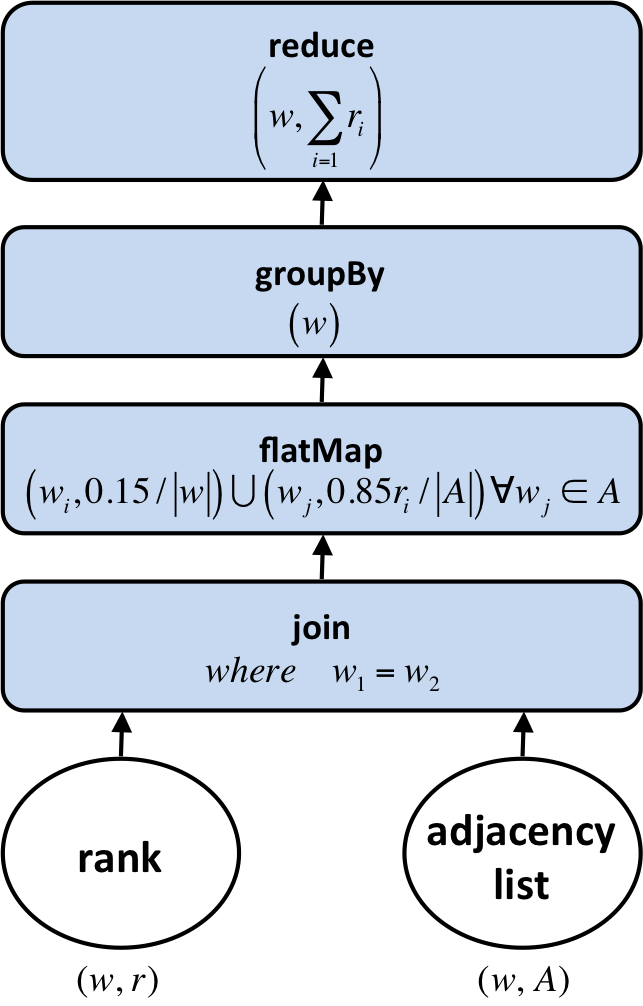
\includegraphics[width=.3\linewidth]{images/pageRankStep.png}
	\caption{Data flow of one iteration of the PageRank algorithm for Spark and Stratosphere.}
	\label{fig:pageRankDataFlow}
\end{figure}

\textbf{Experiment}

For comparison, $10$ steps of the PageRank algorithm for varying sizes of the adjacency matrix $A$ are calculated.
The adjacency matrix $A$ is a sparse matrix of size $n \times n$ with a sparsity of $0.001$.
For each test run, the matrix is randomly generated so that their non-zero cell entries are uniformly distributed.
The computation is executed on $50$ cores of the DIMA cluster.
The block size is set to $500 \times 500$ and Breeze is chosen as math back end for Gilbert's distributed execution engines.
The execution times are depicted in \cref{fig:pageRankResults}.

\begin{figure}
	\centering
	\begin{subfigure}[h]{\dualpgfwidth}
		\begin{tikzpicture}
			\begin{loglogaxis}[
				xlabel={Number of vertices $n$},
				ylabel={Execution time $t$ in s},
				legend pos=north west,
				legend entries={Gilbert Spark, Gilbert Stratosphere, Specialized Stratosphere,Specialized Spark},
				width=\dualpgfwidth,
			]
			
			\addplot[blue,
				mark=x,
			] table[
				x=NumVertices,
				y=Time,
			]
			{data/pagerank/pagerankSpark};

			\addplot[red,
				mark=o,
			] table[
				x=NumVertices,
				y=Time,
			]
			{data/pagerank/pagerankStratosphere};

			\addplot[teal,
				mark=diamond,
			] table[
				x=rows,
				y=time,
			]
			{data/pagerank/pagerankBenchStratosphere};

			\addplot[black,
				mark=triangle,
			] table[
				x=rows,
				y=time,
			]
			{data/pagerank/pagerankBenchSpark};
			\end{loglogaxis}
		\end{tikzpicture}
		\caption{}
		\label{fig:pageRankResults}
	\end{subfigure}
	\begin{subfigure}[h]{\dualpgfwidth}
		\begin{tikzpicture}
			\begin{semilogxaxis}[
				xlabel={Number of vertices $n$},
				ylabel={Speedup},
				legend pos=north west,
				legend entries={Specialized Spark, Specialized Stratosphere},
				width=\dualpgfwidth,
			]
			
			\addplot[blue,
				mark=x,
			] table[
				x=NumVertices,
				y=Speedup,
			]
			{data/pagerank/pagerankSpeedupSpark};

			\addplot[red,
				mark=o,
			] table[
				x=NumVertices,
				y=Speedup,
			]
			{data/pagerank/pagerankSpeedupStratosphere};
			\end{semilogxaxis}
		\end{tikzpicture}
		\caption{}
		\label{fig:pageRankSpeedup}
	\end{subfigure}
	\caption{Comparison of Gilbert's PageRank implementation with specialized algorithms on Spark and Stratosphere running on $50$-core cluster. \subref{fig:pageRankResults} Execution time of $10$ steps of the PageRank algorithm depending on the adjacency matrix's size. \subref{fig:pageRankSpeedup} Speedup of specialized algorithms with respect to Gilbert's implementations.}
	\label{fig:pageRankEvaluation}
\end{figure}

The graph shows that the directly implemented PageRank algorithm runs clearly faster than Gilbert's versions of PageRank.
For Stratosphere, we were only able to compute Gilbert's PageRank for $50000$ web sites, before the computation became too slow to execute.
Even though Spark's execution engine showed a similar runtime behavior for $25000 \le n \le 50000$, Spark was able to scale up to $n=100000$.

The specialized algorithms show a better scalability.
For both systems, Spark and Stratosphere, we could compute the PageRank for up to $150000$ web sites.
Interestingly, the Stratosphere system scales better for the specialized algorithm than Spark.
For $n\ge 25000$, Stratosphere shows significant faster execution times.
It is not yet fully clear what causes this difference.
We assume that the fault tolerance mechanism of Spark is responsible for the performance loss.
With increasing number of iterations and data size, Spark also has to increase the lineage information stored for a possible data recovery.
This lineage information costs CPU time and consumes memory.
Since it is not possible to disable the fault-tolerance mechanism, one has to keep this aspect in mind when comparing Stratosphere with Spark.

The speedup of the specialized algorithms with respect to Gilbert's implementations for this experiment is shown in \cref{fig:pageRankSpeedup}.
For $n\le 25000$, the hand-tuned algorithms running on Spark and Stratosphere show a similarly increasing speedup.
The Stratosphere and Spark version achieve a speedup of approximately $14$ and $10$ for $n=50000$, respectively.
For $n\ge 50000$ Spark seems to exhibit a constant speedup.

The performance difference between the specialized algorithm and Gilbert's version can be explained by considering the different execution plans.
As shown in \cref{fig:pageRankDataFlow}, each iteration of the specialized PageRank algorithm comprises one join, one group reduce and one flat map operation.
The flat map operation can be executed without communication between the nodes.
The join and reduce operation requires the data to be sent over the network.
Thus, most of the time should be spent executing the join and reduce operation.

Looking at line $10$ of \cref{lst:gilbertPageRank}, it can be seen that one matrix-vector product, two vector-scalar products and one vector sum have to be computed for each iteration of Gilbert's PageRank algorithm.
Remembering \cref{sec:LinearAlgebraOperations}, we can deduce that all these operations require two cross, two join and one reduce operation.
The two cross operations, where one of the operands is a scalar value, can be realized efficiently by simply broadcasting this value.
However, the two join operations and the reduce operation require to shuffle the available data and thus inflict some serious network communication costs.

Comparing the specialized algorithm with Gilbert's implementation, it can be clearly seen that the high-level linear algebra representation adds three additional operations, with one of them being highly expensive.
Therefore, it is not surprising that the specialized PageRank algorithm performs better.

\subsubsection{\kmeans}

The \kmeans clustering algorithm~\cite{macqueen:1967a} is very popular for cluster analysis in data mining.
The goal of \kmeans is to partition the available $n$ data points into $k$ clusters, where each data point is assigned to the cluster with the nearest mean.
Even though the optimal solution is NP-hard, heuristic algorithms exist to compute approximations.

\textbf{Algorithm}

The standard algorithm alternately assigns the data points to its nearest intermediate cluster and calculates new intermediate cluster centers as the mean of all assigned data points.
The initial cluster centers are usually randomly selected points from the set of data points or random points.
The MATLAB code for the \kmeans algorithm, shown in \cref{lst:kmeansMatlab}, is a little bit cumbersome if one wants to write it down in matrix notation.

\begin{listing}
	\begin{CenteredBox}
		\begin{lstlisting}[language=Matlab,
		commentstyle=\color{black},
		  stringstyle=\color{black},
		  keywordstyle=\color{black}\bfseries,
		  morekeywords={pdist2, repmat, },]
datapoints = load();
centers = load();
mask = repmat((1:numCenters), numDatapoints, 1)';
for i = 1:maxIterations
		distances = pdist2(datapoints, centers);
		assignments = min(distances, [], 2);
		repIdx = repmat(assignments', numCenters, 1);
		multiplier = repIdx == mask;
		divisor = repmat(sum(multiplier, 2), 1, dimension);
		centers = (multiplier*datapoints)./divisor;
end
		\end{lstlisting}
	\end{CenteredBox}
	\caption{MATLAB \kmeans implementation.}
	\label{lst:kmeansMatlab}
\end{listing}

The data points and centers are stored row-wise in the matrices \code{datapoints} and \code{centers}.
The first step, assigning each data point to its nearest center, is done in the lines $5$ and $6$.
The \code{pdist2} function calculates the pairwise euclidean distance between the rows of its two operands, in this case, the current centers and the data points.
Once all pairwise distances have been calculated, the nearest cluster center is selected for each data point.
This computation is done in line $6$.
The \code{assignments} column vector contains the index of the nearest cluster center for each data point.
In order to calculate the new cluster centers as the mean of all assigned data points, some repmat magic has to be introduced.
The idea is to construct for each center a logical row vector which indicates all data points assigned to this cluster.
The computation is achieved by generating a matrix which contains in each row the \code{assignments} vector.
The matrix has as many rows as there are clusters.
The generated matrix is compared with \code{mask} in line $8$, whose cells are set to the row index of the cell.
That gives the aforementioned indicator matrix.
By adding the entries of each row, the number of data points assigned to a cluster center can be computed.
The new cluster centers and thus the second step of the algorithm are obtained as the result of a matrix multiplication and cellwise matrix division in line $10$.	

Compared to the MATLAB representation, the direct implementation for Spark and Stratosphere seems rather simple.
The first difference is that the data points are represented as tuples of the form $(id_i, p_i)$ with $id_i$ being the identifier of data point $i$ and $p_i$ being its coordinates.
The clusters are represented likewise as tuples $(id_j, c_j)$ with $c_j$ being the coordinates of the cluster center.
In order to calculate the pairwise distances between the data points $p_i$ and the clusters $c_j$, the Cartesian product of the two datasets is constructed.
This operation produces all combinations of data point cluster pairs.
Having the coordinates of the data point and the cluster center, the distance can easily be computed.
The output of the distance computation is a tuple of the form $(id_i, p_i, id_j, \norm{p_i - c_j}_2)$, the data point ID, the data point coordinates, the cluster center ID and the distance.
The cluster center with the minimal distance can be selected by grouping on the data point id $id_i$ and selecting the cluster center ID with minimal distance. 
The result of the reduce operation has the form $(id_j, p_i)$ with $id_j$ being the nearest cluster center ID.
In order to calculate the new cluster centers, the current data set has to be grouped on the cluster center ID.
The generated groups contain the data points, which are assigned to the respective cluster center. 
The new cluster centers are computed by adding all data points $p_i$ of each group up and dividing the result by the number of points contained in the groups.
These operations constitute a single iteration step.
The \kmeans algorithm is obtained by repeating the iteration step until the cluster centers converge.
The dataflow plan of a single iteration step is depicted in \cref{fig:kmeansDataflow}.

\begin{figure}
	\centering
	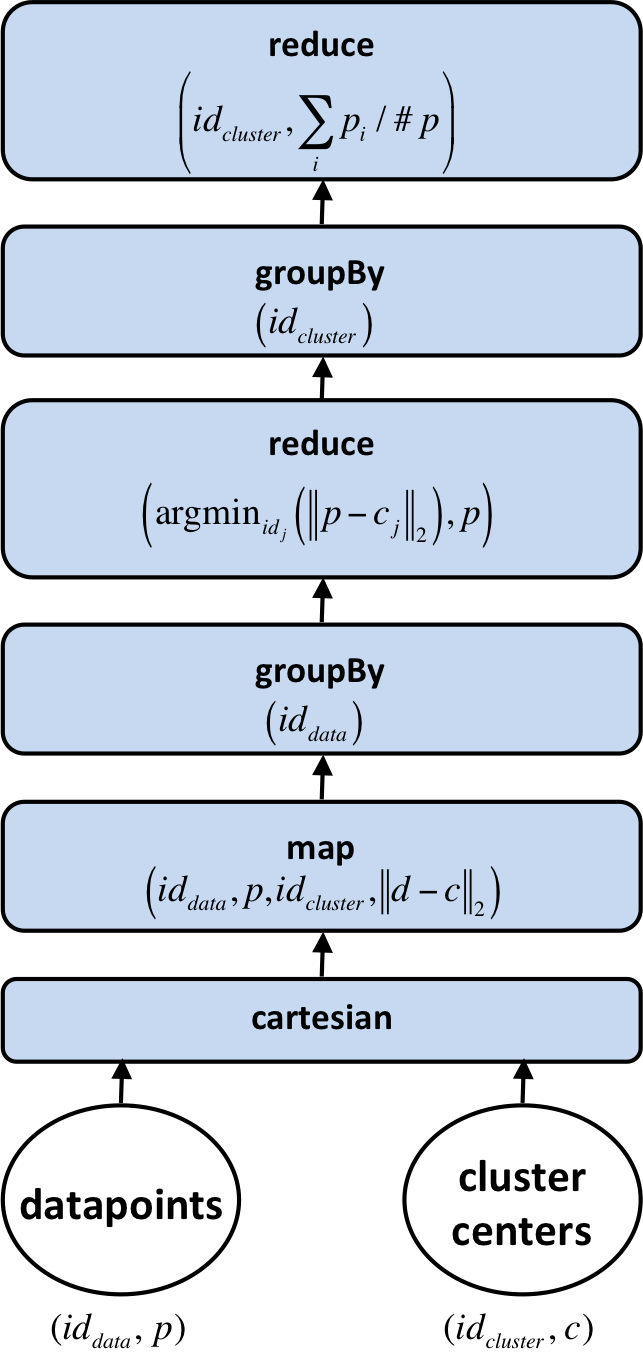
\includegraphics[width=0.3\linewidth]{images/kmeansStep.png}
	\caption{Dataflow plan of a single \kmeans step.}
	\label{fig:kmeansDataflow}
\end{figure}

The execution time of Gilbert's \kmeans implementation is compared with the execution time of the hand-tuned algorithms.
The Gilbert code is given in \cref{lst:kmeansGilbert}.
As it can be seen, the only differences between the MATLAB and Gilbert version are the \code{fixpoint}, the \code{linspace} and the \code{minWithIndex} function.
The \code{linspace} function generates a linearly spaced row vector, as it is known from MATLAB.
The \code{minWithIndex} function returns the minimum value of the specified dimension and its index as column vectors in a cell array.

\begin{listing}
	\begin{CenteredBox}
		\begin{lstlisting}[language=Matlab,
		commentstyle=\color{black},
		  stringstyle=\color{black},
		  keywordstyle=\color{black}\bfseries,
		  morekeywords={repmat, pdist2, minWithIndex, fixpoint}
		  ]
datapoints = load();
centers = load();
mask = repmat(linspace(1, numCenters, numCenters), ...
	numDatapoints, 1)';
function newCenters = kmeansStep(centers)
		distances = pdist2(datapoints, centers);
  	assignments = minWithIndex(distances, 2);
  	repIdx = repmat(assignments{2}', numCenters, 1);
  	multiplier = repIdx == mask;
  	divisor = repmat(sum(multiplier, 2), 1, dimension);
  	newCenters = (multiplier*datapoints)./divisor;
end
fixpoint(centers,@kmeansStep, maxIterations)
		\end{lstlisting}
	\end{CenteredBox}
	\caption{Gilbert \kmeans implementation.}
	\label{lst:kmeansGilbert}
\end{listing}

\subsubsection{Experiment}

For the experiments, $10$ steps of the \kmeans algorithms on the $50$-core DIMA cluster are calculated.
The algorithms compute $100$ cluster centers from $n$ data points.
The points are $2$-dimensional.
The number of data points is varied from $1000$ to $1000000$.
The data points and the initial cluster centers are drawn from a uniform distribution.
The block size is set to $500\times 500$.
The results of the experiment are depicted in \cref{fig:kmeansResult}.

\begin{figure}
	\centering
	\begin{subfigure}[h]{\dualpgfwidth}
		\begin{tikzpicture}
			\begin{loglogaxis}[
				xlabel={Number of data points $n$},
				ymax=5000,
				ylabel={Execution time $t$ in s},
				legend pos=north west,
				legend entries={Gilbert Spark, Gilbert Stratosphere, Specialized Stratosphere},
				width=\dualpgfwidth,
			]
			
			\addplot[blue,
				mark=x,
			] table[
				x=NumDatapoints,
				y=Time,
			]
			{data/kmeans/kmeansSpark};

			\addplot[red,
				mark=o,
			] table[
				x=NumDatapoints,
				y=Time,
			]
			{data/kmeans/kmeansStratosphere};

			\addplot[teal,
				mark=diamond,
			] table[
				x=numDatapoints,
				y=time,
			]
			{data/kmeans/kmeansBenchStratosphere};
			\end{loglogaxis}
		\end{tikzpicture}
		\caption{}
		\label{fig:kmeansResult}
	\end{subfigure}
	\begin{subfigure}[h]{\dualpgfwidth}
		\begin{tikzpicture}
			\begin{semilogxaxis}[
				xlabel={Number of data points $n$},
				ylabel={Speedup},
				legend pos=north west,
				legend entries={Specialized Stratosphere},
				width=\dualpgfwidth,
				ymin=0,
			]
			
			\addplot[red,
				mark=o,
			] table[
				x=NumDatapoints,
				y=Speedup,
			]
			{data/kmeans/kmeansSpeedupStratosphere};
			\end{semilogxaxis}
		\end{tikzpicture}
		\caption{}
		\label{fig:kmeansSpeedup}
	\end{subfigure}
	\caption{Comparison of Gilbert's \kmeans implementation with specialized algorithm on Stratosphere. \subref{fig:kmeansResult} Execution time of $10$ steps of the \kmeans algorithm on $50$-cores depending on the adjacency matrix's size. \subref{fig:kmeansSpeedup} Speedup of specialized algorithm with respect to Gilbert's implementation on Stratosphere.}
	\label{fig:kmeansBenchmark}
\end{figure}

We observe that Gilbert's \kmeans implementations perform more slowly than the specialized implementation.
We could only calculate $100000$ points with Gilbert, because the computation took too long to finish for more points.
The speedup of the specialized algorithm with respect to Stratosphere's execution engine is shown in \cref{fig:kmeansSpeedup}.
With an increasing number of data points $n$, the speedup increases monotonically.
For $n=100000$ the specialized implementation achieves a speedup of $8$ and $10$ compared to the Spark executor and Stratosphere executor, respectively.
Thus, we can conclude that the specialized algorithm of \kmeans executing on Stratosphere not only runs faster but also scales better than Gilbert's implementations.
Interestingly, we were not able to run the specialized algorithm on Spark because the two reduce operations caused the system to become unbearably slow.

If we take a closer look at the execution plans of both algorithms, it becomes clear why Gilbert performs so poorly.
For each step of the specialized algorithm, the dataflow system has to execute one Cartesian, one map and two group reduce operations.
The two group reduce and the Cartesian operation are responsible for most of the work load, because they cause significant network I/O.

For Gilbert, the execution plan is more complex.
Looking at the iteration step in \cref{lst:kmeansGilbert}, the following summation is obtained:
The \code{pdist2} function is implemented using one join, one map and one group reduce operation.
The \code{minWithIndex} function uses three Cartesian, one group reduce and two cogroup operations.
The \code{repmat} function comprises three Cartesian and one cogroup operation.
The comparison operator in line $9$ requires one join operation.
The matrix multiplication and cellwise matrix division in line $11$ is implemented using two join and one reduce operation.
In total, one step of Gilbert's \kmeans algorithm inflicts four join, nine Cartesian, four cogroup and three group reduce operations.
Consequently, it can be concluded that the linear algebra abstraction of Gilbert comes at the price of a more complex and thus longer running execution plan.

\section{Breeze vs. Mahout Math-Backend}

As we have explained in \cref{sec:mathBackend}, Gilbert supports two math back ends for the computation of local tasks.
The principal math back end uses the Breeze library for high performance linear algebra operations.
As an alternative, Gilbert also supports the popular Mahout math library.

As first benchmark, the matrix multiplication from \cref{subsec:mm} is repeated with the Mahout library.
The benchmark calculates the matrix multiplication of two sparse matrices $A,B\in\mathbb{R}^{n\times n}$ with $n$ being their dimensionality.
The matrices have a sparsity of $0.001$.
The computation is executed on $50$ cores and we use a block size of $500\times 500$.
The results are given in \cref{subfig:mmMathBackend}.

\begin{figure}
	\centering
	\begin{subfigure}{\dualpgfwidth}
		\begin{tikzpicture}
			\begin{semilogxaxis}[
				xlabel={Dimensionality $n$},
				ylabel={Execution time $t$ in s},
				legend pos=north west,
				legend entries={Breeze Spark, Breeze Stratosphere, Mahout Spark, Mahout Stratosphere},
				width=\dualpgfwidth,
				xtick=data,
				log ticks with fixed point,
			]
			
			\addplot[
				color=red,
				mark=o,
			] table[
				x=RowsA,
				y=Time,
			]
			{data/matrixMultLoad/matrixMultBreezeLoadSpark};
			
			\addplot[
				color=teal,
				mark=triangle,
			]table[
				x=RowsA,
				y=Time,
			]
			{data/matrixMultLoad/matrixMultBreezeLoadStratosphere};

			\addplot[
				color=blue,
				mark=x,
			] table[
				x=RowsA,
				y=Time,
			]
			{data/matrixMultLoad/matrixMultMahoutLoadSpark};

			\addplot[
				color=black,
				mark=diamond,
			]table[
				x=RowsA,
				y=Time,
			]
			{data/matrixMultLoad/matrixMultMahoutLoadStratosphere};
			
			\end{semilogxaxis}
		\end{tikzpicture}
		\caption{}
		\label{subfig:mmMathBackend}
	\end{subfigure}
	\begin{subfigure}{\dualpgfwidth}
		\begin{tikzpicture}
			\begin{semilogxaxis}[
				xlabel={Rows $d$ of $V$},
				ylabel={Execution time $t$ in s},
				legend pos=north west,
				legend entries={Breeze Spark, Breeze Stratosphere, Mahout Spark, Mahout Stratosphere},
				width=\dualpgfwidth,
			]
			
			\addplot[
				color=red,
				mark=o,
			] table[
				x=Rows,
				y=Time,
			]
			{data/nnmfStepLoad/nnmfStepBreezeLoadSpark};
			
			\addplot[
				color=teal,
				mark=triangle,
			]table[
				x=Rows,
				y=Time,
			]
			{data/nnmfStepLoad/nnmfStepBreezeLoadStratosphere};

			\addplot[
				color=blue,
				mark=x,
			] table[
				x=Rows,
				y=Time,
			]
			{data/nnmfStepLoad/nnmfStepMahoutLoadSpark};

			\addplot[
				color=black,
				mark=diamond,
			]table[
				x=Rows,
				y=Time,
			]
			{data/nnmfStepLoad/nnmfStepMahoutLoadStratosphere};
			
			\end{semilogxaxis}
		\end{tikzpicture}
		\caption{}
		\label{subfig:nmfMathBackend}
	\end{subfigure}
	\caption{Comparison of Breeze and Mahout math back end. \subref{subfig:mmMathBackend} Runtime of matrix multiplication on $50$-core cluster depending on the dimensionality $n$ using Breeze and Mahout. \subref{subfig:nmfMathBackend} Runtime of single GNMF step on $50$-core cluster depending on the number of rows $d$ of $V$ using Breeze and Mahout.}
	\label{fig:nnmfLoadMathBackend}
\end{figure}

The results of the matrix multiplication demonstrate impressively that Breeze is far superior to Mahout in multiplying two sparse matrices.
Even for relatively small matrix sizes, the execution times differ strikingly.
For $n=2500$, Spark's and Stratosphere's execution engine using the Mahout library take 723 seconds and 745 seconds to finish the computation, respectively.
By contrast, the same computation using the Breeze library finishes after 10 seconds and 71 seconds on Spark and Stratosphere, respectively.
The performance gap even widens for an increasing dimensionality $n$.
For $n=5000$, Breeze reaches a speedup of $275$ compared to Mahout on Spark.
It can be concluded that even for small matrix sizes the multiplication using Mahout is almost infeasible.

The mystery of this bad performance can be unraveled by taking a look into the source code of Mahout.
Mahout offers a sparse matrix implementation, based on hash maps.
However, it does not provide an efficient algorithm for this data structure.
Instead, Mahout uses the standard matrix multiplication algorithm.
Thus, for each resulting element $c_{i,j}$, Mahout iterates over the complete row $a_i$ of $A$ and column $b^{j}$ of $B$, even though most of the row and column entries will be zero.
Even worse, each access triggers an hash map look up.
In total, the matrix multiplication has to perform $2n^3$ hash table look ups and $n^3$ hash table insertions.

In contrast to Mahout, Breeze implements the sparse matrix using the compressed sparse column (CSC) storing scheme, which stores the data in a continuous array.
This approach not only avoids costly hash map look ups, but Breeze also implements an optimized matrix multiplication algorithm for CSC.
The algorithm is aware of the sparse nature of its operands and accesses only elements which are non-zero in both matrices.

As second benchmark, we repeated the GNMF computation from \cref{subsec:NMF}.
We calculated a single GNMF step for varying number of rows $d$ of $V$ on $50$-cores of our cluster.
The number of rows $d$ reaches from $500$ to $10000$.
As before, the sparsity of $V$ is $0.001$ and its non-zero cells are distributed uniformly.
The sizes of $W$ and $H$ are $d\times 10$ and $10 \times 100000$, respectively.
For the benchmark, we set the block size to $500 \times 500$.
The runtimes of the Breeze and Mahout math back end are given in \cref{subfig:nmfMathBackend}.

It can be clearly seen that GNMF runs faster with Breeze as math back end on the Stratosphere as well as on the Spark execution engine.
On Spark, Breeze reaches a speedup of roughly $4$ for $d=10000$. 
On Stratosphere, Breeze reaches a speedup of about $1.75$ for the same number of rows.

We can conclude that Breeze has a better support for sparse matrix operations.
Breeze also performs better for operations on mixed sparse and dense matrices as it is the case for GNMF.
However, the gap is not as striking as it is the case for sparse matrix operations only.
In conclusion, we highly recommend using Breeze as the math back end in order to experience best performance with Gilbert programs.


%!TEX root=main.tex
\section{Conclusion}
\label{cha:conclusion}

In the context of this thesis, we addressed the problem of managing and exploiting the ever increasing data flood.
In contrast to ever growing gathering and storage capacities, the tools to harness the collected information did not scale accordingly.
Our current analytic tools are mostly limited to data sizes which can be kept in the memory of a single machine.
Often analysts have to reduce data to make them processable, thereby missing valuable insights.
In order to analyze petabytes of data, the only viable solution is to split the work up and execute it in parallel.
However, parallel data processing is a highly complex and error-prone task.
Not only does it distract the analyst from its actual task but it also requires as skill set hardly anyone possesses.
Thus, having analytic tools, which scale to vast amounts of data while hiding the low-level implementation details, becomes an imperative.

Gilbert tackles the aforementioned problems by fusing the assets of high-level linear algebra abstractions with the power of massively parallel dataflow systems.
Gilbert is a fully functional linear algebra environment, which is programmed by the widespread MATLAB language.
Gilbert programs are executed on massively parallel dataflow systems, which allow to process data exceeding the capacity of a single computer's memory.
Gilbert only requires the user to program MATLAB code in order to use the system.
Consequently, it is usable by a wide audience of data scientists, who can easily switch to Gilbert without having to re-adapt.
These properties make Gilbert a suitable candidate for the data processing challenges of tomorrow.

Gilbert itself comprises the technology stack to parse, type and compile MATLAB code into a format which can be executed in parallel.
In order to apply high-level linear algebra optimizations, we conceived an intermediate representation for linear algebra programs.
Gilbert's optimizer exploits this representation to remove redundant transpose operations and to determine an optimal matrix multiplication order.
The optimized program is translated into an highly optimized execution plan suitable for the execution on a supported engine.
Gilbert allows the distributed execution on Spark and Stratosphere.
Additionally, it exists a local execution mode.
Gilbert was developed to be easily extensible with new execution engines.
For the local linear algebra operations the Gilbert user can choose between the Breeze and Mahout library.

Our systematical evaluation has shown that Gilbert supports all fundamental linear algebra operations, making it fully operational.
Additionally, its loop support allows to implement a wide multitude of machine learning algorithms within Gilbert.
Exemplary, we have implemented the PageRank, \kmeans and GNMF algorithm.
The code changes required to make these algorithms run in Gilbert are minimal and only concern Gilbert's loop abstraction.
Our evaluation has demonstrated the effectiveness of Gilbert's matrix multiplication reordering optimization.
Furthermore, we could observe that the matrix blocking size has strong implications on the overall performance.
The best performance is achieved with block sizes which offer a good compromise between data parallelism and data granularity.
Our benchmarks have proved that Gilbert can handle data sizes which no longer can be efficiently processed on a single computer.
Moreover, Gilbert showed a promising scale out behavior, making it a suitable candidate for large-scale data processing.

The key contributions of this thesis include the development of a scalable data analysis tool which can be programmed using the well-known MATLAB language.
That way, we made the world of distributed computing accessible for data scientists and people concerned with machine learning.
Furthermore, we researched how to implement linear algebra operations efficiently in modern parallel data flow systems, such as Spark and Stratosphere.
In line with that research was the investigation of suitable distributed data structures for the representation of matrices and vectors.
As part of the implementation of Gilbert, we also investigated how to add automatically type information to MATLAB code using a type inference mechanism.
Type inference ensures a minimally invasive approach, since the user does not have to add additional statements to his code.
Last but not least, we showed the effectiveness of a cost-based optimizer for linear algebra programs.

We also noted some limitations of Gilbert.
The proposed Hindley-Milner type inference algorithm turned out to have problems resolving polymorphic types.
As a consequence, Gilbert will incorrectly reject some well-typed programs.
However, these programs constitute only corner cases.
Even though, Gilbert can process vast amounts of data, it turned out that it cannot beat the performance of hand-tuned algorithms using Spark or Stratosphere.
Considering the overhead the linear algebra abstraction entails, this fact is not really surprising, though.
The overhead is also the reason for the higher memory foot-print, causing Spark and Stratosphere to spill faster to disk than the hand-tuned algorithms.
Consequently, the processable problem sizes are smaller.
Gilbert trades some performance off for better usability, which manifests itself in shorter and more expressive programming code.
The fact that Gilbert only supports one hard-wired partitioning scheme, namely square blocks, omits possible optimization potential.
Another limitation are the error messages of the parsing, typing and compilation phase.
It is a well known problem of the HM type inference algorithm that in case of typing errors the original error source is hard to locate.
The same holds true for issued error messages by Scala's Parser Combinators.

Interesting aspects for further research and improvements of Gilbert include the extension of the Gilbert optimizer by new optimization strategies.
The investigation of different matrix partitioning schemes and its integration into the optimizer which selects the best overall partitioning seems to be very promising.
Furthermore, a tighter coupling of Gilbert's optimizer with Stratosphere's optimizer could result in beneficial synergies.
Forwarding the inferred matrix sizes to the underlying execution system might help to improve the execution plans.
The numerical stability of Gilbert's computations is another important aspect, which has been completely left out in the context of this thesis.
However, any linear algebra environment has to guarantee numerical stability which might be influenced by Gilbert's parallel execution.
Therefore, the numerical stability of Gilbert deserves its own separate evaluation.
As stated above, the HM inference algorithm has problems with polymorphic types.
In our opinion, it is worthwhile to look into other type inference algorithms, such as the type inference system of Haskell~\cite{haskell}, to assess whether they are better suited to automatically annotate Matlab with type information.
We also strongly advise to add support for further execution engines to Gilbert.
An appropriate candidate could be the H2O~\cite{h2o} data processing engine.
Additionally, it is always beneficial to extend the set of implemented algorithms and to probe them at a large data scale.

In conclusion, we have developed Gilbert, a sparse linear algebra environment executed in massively parallel dataflow systems.
Gilbert transparently parallelizes sequential linear algebra code.
Thus, Gilbert makes it blindingly easy to develop parallel analytic tools which are capable of processing vast amounts of data.
With Gilbert at hand, we are well prepared for the looming challenges of today and tomorrow.
We believe that our system helps mankind to benefit a little bit more from the world of data.

% \section{Verwendung}
% Die GI gibt unter \url{http://www.gi-ev.de/LNI} Vorgaben für die Formatierung von Dokumenten in der LNI Reihe.
% Für \LaTeX-Dokumente werden diese durch die Dokumentenklasse \texttt{lni} realisiert.

% Dieses Dokument basiert auf der offiziellen Dokumentation, aber wurde entsprechend der aktuellen Vorlage und den eingebundenen Paketen aktualisiert.
% Die aktuelle Version wird unter \url{https://github.com/latextemplates/LNI} gepflegt.
% Es werden (nach Möglichkeit) die aktuellen Versionen von der GI eingebunden.

% Diese Dokumentation simplifiziert und setzt grundlegendes LaTeX-Wissen voraus.
% Es werden generische Platzhalter an die entsprechenden Stellen (wie Beispielsweise Author) gesetzt und nicht weiter an anderer Stelle dokumentiert.

% Dieses Template ist wie folgt gegliedert:
% \Cref{sec:demos} zeigt Demonstrationen der Verbesserung von GitHub-LNI gegenüber der originalen Vorlage.
% \Cref{sec:lniconformance} zeigt die Einhaltung der Richtlinien durch einfachen Text.
% \Cref{sec:monographien} enthält Hinweise für Monographien. Diese kommen zum Einsatz, wenn \emph{kein} Tagungsbandbeitrag verfasst wird, sondern eine Dissertation oder ähnliches.

% \section{Demonstrationen}
% \label{sec:demos}
% The symbol for powerset is now correct: $\powerset$ and not a Weierstrass p ($\wp$).

% Brackets work as designed:
% <test>

% See \href{https://www.ctan.org/pkg/microtype}{microtype} in action here:
% \blindtext

% \section{Demonstration der Einhaltung der Richtlinien}
% \label{sec:lniconformance}

% \subsection{Literaturverzeichnis}
% Der letzte Abschnitt zeigt ein beispielhaftes Literaturverzeichnis für Bücher mit einem Autor \cite{Ez10} und zwei AutorInnen \cite{AB00}, einem Beitrag in Proceedings mit drei AutorInnen \cite{ABC01}, einem Beitrag in einem LNI Band mit mehr als drei AutorInnen \cite{Az09}, zwei Bücher mit den jeweils selben vier AutorInnen im selben Erscheinungsjahr \cite{Wa14} und \cite{Wa14b}, ein Journal \cite{Gl06}, eine Website \cite{GI14} bzw.\ anderweitige Literatur ohne konkrete AutorInnenschaft \cite{XX14}.

% Formatierung und Abkürzungen werden für die Referenzen \texttt{book}, \texttt{inbook}, \texttt{proceedings}, \texttt{inproceedings}, \texttt{article}, \texttt{online} und \texttt{misc} automatisch vorgenommen.
% Mögliche Felder für Referenzen können der Beispieldatei \texttt{paper.bib} entnommen werden.
% Andere Referenzen bzw.\ Felder müssen allenfalls nachträglich angepasst werden.

% \subsection{Abbildungen}
% \Cref{fig:demo} zeigt eine Abbildung.

% \begin{figure}
%   \centering
%   Hier sollte die Graphik mittels \texttt{includegraphics} eingebunden werden.

%   %\includegraphics[width=.8\textwidth]{filename}
%   \caption{Demographik}
%   \label{fig:demo}
% \end{figure}

% \subsection{Tabellen}
% \Cref{tab:demo} zeigt eine Tabelle.

% \begin{table}
% \centering
% \begin{tabular}{lll}
% \toprule
% Überschriftsebenen & Beispiel & Schriftgröße und -art \\
% \midrule
% Titel (linksbündig) & Der Titel \ldots & 14 pt, Fett\\
% Überschrift 1 & 1 Einleitung & 12 pt, Fett\\
% Überschrift 2 & 2.1 Titel & 10 pt, Fett\\
% \bottomrule
% \end{tabular}
% \caption{Die Überschriftsarten}
% \label{tab:demo}
% \end{table}

% \subsection{Programmcode}
% Die LNI-Formatvorlage verlangt die Einrückung von Listings vom linken Rand.
% In der \texttt{lni}-Dokumentenklasse ist dies für die \texttt{verbatim}-Umgebung realisiert.

% \begin{verbatim}
% public class Hello { 
%     public static void main (String[] args) { 
%         System.out.println("Hello World!"); 
%     } 
% } 
% \end{verbatim}

% Alternativ kann auch die \texttt{lstlisting}-Umgebung verwendet werden.

% \Cref{L1} zeigt uns ein Beispiel, das mit Hilfe der \texttt{lstlisting}-Umgebung realisiert ist.

% \lstset{basicstyle=\ttfamily}
% \begin{lstlisting} [captionpos=b, caption=Beschreibung, label=L1, xleftmargin=0.5cm]
% public class Hello { 
%     public static void main (String[] args) { 
%         System.out.println("Hello World!"); 
%     } 
% }
% \end{lstlisting}

% \subsection{Formeln und Gleichungen}

% Die korrekte Einrückung und Nummerierung für Formeln ist bei den Umgebungen \texttt{equation} und \texttt{eqnarray} gewährleistet.

% \begin{equation}
%   1=4-3
% \end{equation}
% und
% \begin{eqnarray}
%   2=7-5\\
%   3=2-1
% \end{eqnarray}

% \section{Hinweise für Monographien}
% \label{sec:monographien}
% Für Proceedings und Seminarbände ist die Seitennummerierung, wenn nicht anders vorgegeben, von den HerausgeberInnen vorzunehmen, die einzelnen Beiträge sind von deren AutorInnen also ohne Seitennummerierung vorzulegen; Monographien und Dissertationen sind von der Autorin/ vom Autor zu nummerieren:
% \begin{itemize}
% \item Vorwort, Inhaltsverzeichnis und Beiträge beginnen grundsätzlich auf einer rechten Seite, ggf.\ ist also eine Leerseite einzufügen.
% \item Die Seitennummer des ersten Beitrages errechnet sich aus der Seitenzahl der \enquote{Startseiten} + 1
% \item Die \enquote{Startseiten} (Muster siehe Anlage in der HerausgeberInnen-Information) bestehen aus:
% \begin{itemize}
% \item 1.\ Seite (rechts): GI-Logo
% \item 2.\ Seite (links): leer
% \item 3.\ Seite (rechts): Titelblatt
% \item 4.\ Seite (links): Bibliographische Angaben
% \item 5.\ Seite ff (rechts): Vorwort
% \item Anschließend an das Vorwort auf neuer Seite (links oder rechts): Angaben zur Tagungsleitung, zum Programmkomitee oder Organisationsteam, etc. Hier können auch Logos von SponsorInnen und VeranstaltungspartnerInnen abgedruckt werden.
% \item Beginnend auf einer rechten (ungerade nummerierten) Seite: Inhaltsverzeichnis
% \end{itemize}
% \end{itemize}

%DO NOT USE \bibliographystyle - is is already done in lni.cls
%\bibliographystyle{lnig}

\bibliography{paper}

\end{document}
